\documentclass[twoside]{book}

% Packages required by doxygen
\usepackage{fixltx2e}
\usepackage{calc}
\usepackage{doxygen}
\usepackage[export]{adjustbox} % also loads graphicx
\usepackage{graphicx}
\usepackage[utf8]{inputenc}
\usepackage{makeidx}
\usepackage{multicol}
\usepackage{multirow}
\PassOptionsToPackage{warn}{textcomp}
\usepackage{textcomp}
\usepackage[nointegrals]{wasysym}
\usepackage[table]{xcolor}

% Font selection
\usepackage[T1]{fontenc}
\usepackage[scaled=.90]{helvet}
\usepackage{courier}
\usepackage{amssymb}
\usepackage{sectsty}
\renewcommand{\familydefault}{\sfdefault}
\allsectionsfont{%
  \fontseries{bc}\selectfont%
  \color{darkgray}%
}
\renewcommand{\DoxyLabelFont}{%
  \fontseries{bc}\selectfont%
  \color{darkgray}%
}
\newcommand{\+}{\discretionary{\mbox{\scriptsize$\hookleftarrow$}}{}{}}

% Page & text layout
\usepackage{geometry}
\geometry{%
  a4paper,%
  top=2.5cm,%
  bottom=2.5cm,%
  left=2.5cm,%
  right=2.5cm%
}
\tolerance=750
\hfuzz=15pt
\hbadness=750
\setlength{\emergencystretch}{15pt}
\setlength{\parindent}{0cm}
\setlength{\parskip}{3ex plus 2ex minus 2ex}
\makeatletter
\renewcommand{\paragraph}{%
  \@startsection{paragraph}{4}{0ex}{-1.0ex}{1.0ex}{%
    \normalfont\normalsize\bfseries\SS@parafont%
  }%
}
\renewcommand{\subparagraph}{%
  \@startsection{subparagraph}{5}{0ex}{-1.0ex}{1.0ex}{%
    \normalfont\normalsize\bfseries\SS@subparafont%
  }%
}
\makeatother

% Headers & footers
\usepackage{fancyhdr}
\pagestyle{fancyplain}
\fancyhead[LE]{\fancyplain{}{\bfseries\thepage}}
\fancyhead[CE]{\fancyplain{}{}}
\fancyhead[RE]{\fancyplain{}{\bfseries\leftmark}}
\fancyhead[LO]{\fancyplain{}{\bfseries\rightmark}}
\fancyhead[CO]{\fancyplain{}{}}
\fancyhead[RO]{\fancyplain{}{\bfseries\thepage}}
\fancyfoot[LE]{\fancyplain{}{}}
\fancyfoot[CE]{\fancyplain{}{}}
\fancyfoot[RE]{\fancyplain{}{\bfseries\scriptsize Generated by Doxygen }}
\fancyfoot[LO]{\fancyplain{}{\bfseries\scriptsize Generated by Doxygen }}
\fancyfoot[CO]{\fancyplain{}{}}
\fancyfoot[RO]{\fancyplain{}{}}
\renewcommand{\footrulewidth}{0.4pt}
\renewcommand{\chaptermark}[1]{%
  \markboth{#1}{}%
}
\renewcommand{\sectionmark}[1]{%
  \markright{\thesection\ #1}%
}

% Indices & bibliography
\usepackage{natbib}
\usepackage[titles]{tocloft}
\setcounter{tocdepth}{3}
\setcounter{secnumdepth}{5}
\makeindex

% Hyperlinks (required, but should be loaded last)
\usepackage{ifpdf}
\ifpdf
  \usepackage[pdftex,pagebackref=true]{hyperref}
\else
  \usepackage[ps2pdf,pagebackref=true]{hyperref}
\fi
\hypersetup{%
  colorlinks=true,%
  linkcolor=blue,%
  citecolor=blue,%
  unicode%
}

% Custom commands
\newcommand{\clearemptydoublepage}{%
  \newpage{\pagestyle{empty}\cleardoublepage}%
}

\usepackage{caption}
\captionsetup{labelsep=space,justification=centering,font={bf},singlelinecheck=off,skip=4pt,position=top}

%===== C O N T E N T S =====

\begin{document}

% Titlepage & ToC
\hypersetup{pageanchor=false,
             bookmarksnumbered=true,
             pdfencoding=unicode
            }
\pagenumbering{alph}
\begin{titlepage}
\vspace*{7cm}
\begin{center}%
{\Large I\+GoR }\\
\vspace*{1cm}
{\large Generated by Doxygen 1.8.13}\\
\end{center}
\end{titlepage}
\clearemptydoublepage
\pagenumbering{roman}
\tableofcontents
\clearemptydoublepage
\pagenumbering{arabic}
\hypersetup{pageanchor=true}

%--- Begin generated contents ---
\chapter{Deprecated List}
\label{deprecated}
\Hypertarget{deprecated}

\begin{DoxyRefList}
\item[\label{deprecated__deprecated000001}%
\Hypertarget{deprecated__deprecated000001}%
Member \hyperlink{classGenModel_a72c20c4c6d81b5c464bffad5acd36286}{Gen\+Model\+:\+:generate\+\_\+sequences} (int, bool)]This function used to store generated sequences in memory, and quickly overloaded it for large number of generated sequences. 
\end{DoxyRefList}
\chapter{Bug List}
\label{bug}
\Hypertarget{bug}

\begin{DoxyRefList}
\item[\label{bug__bug000002}%
\Hypertarget{bug__bug000002}%
Member \hyperlink{classDinucl__markov_a63fd37e31c3e32fee54dc26146bc3fac}{Dinucl\+\_\+markov\+:\+:add\+\_\+to\+\_\+marginals} (long double, Marginal\+\_\+array\+\_\+p \&) const]Will only count realizations of unambiguous nucleotides (realization indices$>$=0 since they are set to -\/1 in iterate\+\_\+common) 
\end{DoxyRefList}
\chapter{Hierarchical Index}
\section{Class Hierarchy}
This inheritance list is sorted roughly, but not completely, alphabetically\+:\begin{DoxyCompactList}
\item \contentsline{section}{Adjacency\+\_\+list}{\pageref{structAdjacency__list}}{}
\item \contentsline{section}{Aligner}{\pageref{classAligner}}{}
\item \contentsline{section}{Alignment\+\_\+data}{\pageref{structAlignment__data}}{}
\item \contentsline{section}{C\+D\+R3\+Seq\+Data}{\pageref{classCDR3SeqData}}{}
\item \contentsline{section}{Counter}{\pageref{classCounter}}{}
\begin{DoxyCompactList}
\item \contentsline{section}{Best\+\_\+scenarios\+\_\+counter}{\pageref{classBest__scenarios__counter}}{}
\item \contentsline{section}{Coverage\+\_\+err\+\_\+counter}{\pageref{classCoverage__err__counter}}{}
\item \contentsline{section}{Errors\+\_\+counter}{\pageref{classErrors__counter}}{}
\item \contentsline{section}{Pgen\+\_\+counter}{\pageref{classPgen__counter}}{}
\end{DoxyCompactList}
\item \contentsline{section}{D\+\_\+position\+\_\+comparator}{\pageref{structD__position__comparator}}{}
\item \contentsline{section}{Enum\+\_\+fast\+\_\+memory\+\_\+dual\+\_\+key\+\_\+map$<$ K1, K2, V $>$}{\pageref{classEnum__fast__memory__dual__key__map}}{}
\item \contentsline{section}{Enum\+\_\+fast\+\_\+memory\+\_\+map$<$ K, V $>$}{\pageref{classEnum__fast__memory__map}}{}
\item \contentsline{section}{Error\+\_\+rate}{\pageref{classError__rate}}{}
\begin{DoxyCompactList}
\item \contentsline{section}{Hypermutation\+\_\+full\+\_\+\+Nmer\+\_\+errorrate}{\pageref{classHypermutation__full__Nmer__errorrate}}{}
\item \contentsline{section}{Hypermutation\+\_\+global\+\_\+errorrate}{\pageref{classHypermutation__global__errorrate}}{}
\item \contentsline{section}{Single\+\_\+error\+\_\+rate}{\pageref{classSingle__error__rate}}{}
\end{DoxyCompactList}
\item \contentsline{section}{Event\+\_\+comparator}{\pageref{structEvent__comparator}}{}
\item \contentsline{section}{Event\+\_\+realization}{\pageref{structEvent__realization}}{}
\item \contentsline{section}{Extract\+Features}{\pageref{classExtractFeatures}}{}
\item \contentsline{section}{gen\+\_\+\+C\+D\+R3\+\_\+data}{\pageref{structgen__CDR3__data}}{}
\item \contentsline{section}{Gen\+Model}{\pageref{classGenModel}}{}
\item \contentsline{section}{std\+:\+:hash$<$ Event\+\_\+safety $>$}{\pageref{structstd_1_1hash_3_01Event__safety_01_4}}{}
\item \contentsline{section}{std\+:\+:hash$<$ Gene\+\_\+class $>$}{\pageref{structstd_1_1hash_3_01Gene__class_01_4}}{}
\item \contentsline{section}{std\+:\+:hash$<$ Int\+\_\+\+Str $>$}{\pageref{structstd_1_1hash_3_01Int__Str_01_4}}{}
\item \contentsline{section}{std\+:\+:hash$<$ Seq\+\_\+type $>$}{\pageref{structstd_1_1hash_3_01Seq__type_01_4}}{}
\item \contentsline{section}{std\+:\+:hash$<$ std\+:\+:pair$<$ Gene\+\_\+class, Seq\+\_\+side $>$ $>$}{\pageref{structstd_1_1hash_3_01std_1_1pair_3_01Gene__class_00_01Seq__side_01_4_01_4}}{}
\item \contentsline{section}{std\+:\+:hash$<$ std\+:\+:pair$<$ Seq\+\_\+type, Seq\+\_\+side $>$ $>$}{\pageref{structstd_1_1hash_3_01std_1_1pair_3_01Seq__type_00_01Seq__side_01_4_01_4}}{}
\item \contentsline{section}{std\+:\+:hash$<$ std\+:\+:tuple$<$ Event\+\_\+type, Gene\+\_\+class, Seq\+\_\+side $>$ $>$}{\pageref{structstd_1_1hash_3_01std_1_1tuple_3_01Event__type_00_01Gene__class_00_01Seq__side_01_4_01_4}}{}
\item \contentsline{section}{inverse\+\_\+offset\+\_\+comparator}{\pageref{structinverse__offset__comparator}}{}
\item \contentsline{section}{Matrix$<$ T $>$}{\pageref{structMatrix}}{}
\item \contentsline{section}{Matrix$<$ double $>$}{\pageref{structMatrix}}{}
\item \contentsline{section}{Model\+\_\+marginals}{\pageref{classModel__marginals}}{}
\item \contentsline{section}{Model\+\_\+\+Parms}{\pageref{classModel__Parms}}{}
\item \contentsline{section}{null\+\_\+delete$<$ T $>$}{\pageref{structnull__delete}}{}
\item \contentsline{section}{offset\+\_\+comp}{\pageref{structoffset__comp}}{}
\item \contentsline{section}{Rec\+\_\+\+Event}{\pageref{classRec__Event}}{}
\begin{DoxyCompactList}
\item \contentsline{section}{Deletion}{\pageref{classDeletion}}{}
\item \contentsline{section}{Dinucl\+\_\+markov}{\pageref{classDinucl__markov}}{}
\item \contentsline{section}{Gene\+\_\+choice}{\pageref{classGene__choice}}{}
\item \contentsline{section}{Insertion}{\pageref{classInsertion}}{}
\end{DoxyCompactList}
\item vector\begin{DoxyCompactList}
\item \contentsline{section}{Int\+\_\+\+Str}{\pageref{classInt__Str}}{}
\end{DoxyCompactList}
\end{DoxyCompactList}

\chapter{Class Index}
\section{Class List}
Here are the classes, structs, unions and interfaces with brief descriptions\+:\begin{DoxyCompactList}
\item\contentsline{section}{\hyperlink{structAdjacency__list}{Adjacency\+\_\+list} \\*I\+GoR\textquotesingle{}s Bayesian Network adjacency list }{\pageref{structAdjacency__list}}{}
\item\contentsline{section}{\hyperlink{classAligner}{Aligner} \\*A modified Smith-\/\+Waterman alignment class }{\pageref{classAligner}}{}
\item\contentsline{section}{\hyperlink{structAlignment__data}{Alignment\+\_\+data} \\*Stores information on the alignment of one genomic template against the target }{\pageref{structAlignment__data}}{}
\item\contentsline{section}{\hyperlink{classBest__scenarios__counter}{Best\+\_\+scenarios\+\_\+counter} \\*Records the N best scenarios realizations and mismatches }{\pageref{classBest__scenarios__counter}}{}
\item\contentsline{section}{\hyperlink{classCDR3SeqData}{C\+D\+R3\+Seq\+Data} \\*Class to store C\+D\+R3 information of a sequence }{\pageref{classCDR3SeqData}}{}
\item\contentsline{section}{\hyperlink{classCounter}{Counter} \\*Scenario statistics recording abstract class }{\pageref{classCounter}}{}
\item\contentsline{section}{\hyperlink{classCoverage__err__counter}{Coverage\+\_\+err\+\_\+counter} \\*Records the number of time each genomic position is observed with or without error }{\pageref{classCoverage__err__counter}}{}
\item\contentsline{section}{\hyperlink{structD__position__comparator}{D\+\_\+position\+\_\+comparator} }{\pageref{structD__position__comparator}}{}
\item\contentsline{section}{\hyperlink{classDeletion}{Deletion} \\*\hyperlink{classDeletion}{Deletion} recombination event }{\pageref{classDeletion}}{}
\item\contentsline{section}{\hyperlink{classDinucl__markov}{Dinucl\+\_\+markov} \\*Dinucleotide insertion Markov model }{\pageref{classDinucl__markov}}{}
\item\contentsline{section}{\hyperlink{classEnum__fast__memory__dual__key__map}{Enum\+\_\+fast\+\_\+memory\+\_\+dual\+\_\+key\+\_\+map$<$ K1, K2, V $>$} }{\pageref{classEnum__fast__memory__dual__key__map}}{}
\item\contentsline{section}{\hyperlink{classEnum__fast__memory__map}{Enum\+\_\+fast\+\_\+memory\+\_\+map$<$ K, V $>$} }{\pageref{classEnum__fast__memory__map}}{}
\item\contentsline{section}{\hyperlink{classError__rate}{Error\+\_\+rate} \\*Abstract class for generic error models behavior }{\pageref{classError__rate}}{}
\item\contentsline{section}{\hyperlink{classErrors__counter}{Errors\+\_\+counter} \\*\hyperlink{classCounter}{Counter} recording the number of genomic nucleotides and errors/mismatch per scenario }{\pageref{classErrors__counter}}{}
\item\contentsline{section}{\hyperlink{structEvent__comparator}{Event\+\_\+comparator} }{\pageref{structEvent__comparator}}{}
\item\contentsline{section}{\hyperlink{structEvent__realization}{Event\+\_\+realization} \\*Unit that stores an event realization name, value and index }{\pageref{structEvent__realization}}{}
\item\contentsline{section}{\hyperlink{classExtractFeatures}{Extract\+Features} \\*Class to extract sequences features (e.\+g. C\+D\+R3) of sequences using alignment and V, J anchors information }{\pageref{classExtractFeatures}}{}
\item\contentsline{section}{\hyperlink{structgen__CDR3__data}{gen\+\_\+\+C\+D\+R3\+\_\+data} }{\pageref{structgen__CDR3__data}}{}
\item\contentsline{section}{\hyperlink{classGene__choice}{Gene\+\_\+choice} \\*Gene\+Choice recombination event }{\pageref{classGene__choice}}{}
\item\contentsline{section}{\hyperlink{classGenModel}{Gen\+Model} \\*High level V(\+D)J generative model }{\pageref{classGenModel}}{}
\item\contentsline{section}{\hyperlink{structstd_1_1hash_3_01Event__safety_01_4}{std\+::hash$<$ Event\+\_\+safety $>$} }{\pageref{structstd_1_1hash_3_01Event__safety_01_4}}{}
\item\contentsline{section}{\hyperlink{structstd_1_1hash_3_01Gene__class_01_4}{std\+::hash$<$ Gene\+\_\+class $>$} }{\pageref{structstd_1_1hash_3_01Gene__class_01_4}}{}
\item\contentsline{section}{\hyperlink{structstd_1_1hash_3_01Int__Str_01_4}{std\+::hash$<$ Int\+\_\+\+Str $>$} }{\pageref{structstd_1_1hash_3_01Int__Str_01_4}}{}
\item\contentsline{section}{\hyperlink{structstd_1_1hash_3_01Seq__type_01_4}{std\+::hash$<$ Seq\+\_\+type $>$} }{\pageref{structstd_1_1hash_3_01Seq__type_01_4}}{}
\item\contentsline{section}{\hyperlink{structstd_1_1hash_3_01std_1_1pair_3_01Gene__class_00_01Seq__side_01_4_01_4}{std\+::hash$<$ std\+::pair$<$ Gene\+\_\+class, Seq\+\_\+side $>$ $>$} }{\pageref{structstd_1_1hash_3_01std_1_1pair_3_01Gene__class_00_01Seq__side_01_4_01_4}}{}
\item\contentsline{section}{\hyperlink{structstd_1_1hash_3_01std_1_1pair_3_01Seq__type_00_01Seq__side_01_4_01_4}{std\+::hash$<$ std\+::pair$<$ Seq\+\_\+type, Seq\+\_\+side $>$ $>$} }{\pageref{structstd_1_1hash_3_01std_1_1pair_3_01Seq__type_00_01Seq__side_01_4_01_4}}{}
\item\contentsline{section}{\hyperlink{structstd_1_1hash_3_01std_1_1tuple_3_01Event__type_00_01Gene__class_00_01Seq__side_01_4_01_4}{std\+::hash$<$ std\+::tuple$<$ Event\+\_\+type, Gene\+\_\+class, Seq\+\_\+side $>$ $>$} }{\pageref{structstd_1_1hash_3_01std_1_1tuple_3_01Event__type_00_01Gene__class_00_01Seq__side_01_4_01_4}}{}
\item\contentsline{section}{\hyperlink{classHypermutation__full__Nmer__errorrate}{Hypermutation\+\_\+full\+\_\+\+Nmer\+\_\+errorrate} \\*A non-\/additive context dependent hypermutation model }{\pageref{classHypermutation__full__Nmer__errorrate}}{}
\item\contentsline{section}{\hyperlink{classHypermutation__global__errorrate}{Hypermutation\+\_\+global\+\_\+errorrate} \\*An additive (independent site) context dependent hypermutation model }{\pageref{classHypermutation__global__errorrate}}{}
\item\contentsline{section}{\hyperlink{classInsertion}{Insertion} \\*\hyperlink{classInsertion}{Insertion} recombination events }{\pageref{classInsertion}}{}
\item\contentsline{section}{\hyperlink{classInt__Str}{Int\+\_\+\+Str} }{\pageref{classInt__Str}}{}
\item\contentsline{section}{\hyperlink{structinverse__offset__comparator}{inverse\+\_\+offset\+\_\+comparator} }{\pageref{structinverse__offset__comparator}}{}
\item\contentsline{section}{\hyperlink{structMatrix}{Matrix$<$ T $>$} }{\pageref{structMatrix}}{}
\item\contentsline{section}{\hyperlink{classModel__marginals}{Model\+\_\+marginals} \\*Encapsulates the marginal probabilities/posterior frequency for each recombination event\textquotesingle{}s realization }{\pageref{classModel__marginals}}{}
\item\contentsline{section}{\hyperlink{classModel__Parms}{Model\+\_\+\+Parms} \\*Implements I\+GoR\textquotesingle{}s Bayesian Network structure }{\pageref{classModel__Parms}}{}
\item\contentsline{section}{\hyperlink{structnull__delete}{null\+\_\+delete$<$ T $>$} \\*Declare a \hyperlink{structnull__delete}{null\+\_\+delete} function }{\pageref{structnull__delete}}{}
\item\contentsline{section}{\hyperlink{structoffset__comp}{offset\+\_\+comp} }{\pageref{structoffset__comp}}{}
\item\contentsline{section}{\hyperlink{classPgen__counter}{Pgen\+\_\+counter} \\*Estimates sequences generation probability }{\pageref{classPgen__counter}}{}
\item\contentsline{section}{\hyperlink{classRec__Event}{Rec\+\_\+\+Event} \\*Recombination event class (I\+GoR\textquotesingle{}s graph nodes) }{\pageref{classRec__Event}}{}
\item\contentsline{section}{\hyperlink{classSingle__error__rate}{Single\+\_\+error\+\_\+rate} \\*Independent single nucleotide error model }{\pageref{classSingle__error__rate}}{}
\end{DoxyCompactList}

\chapter{Class Documentation}
\hypertarget{structAdjacency__list}{}\section{Adjacency\+\_\+list Struct Reference}
\label{structAdjacency__list}\index{Adjacency\+\_\+list@{Adjacency\+\_\+list}}


I\+GoR\textquotesingle{}s Bayesian Network adjacency list.  




{\ttfamily \#include $<$Model\+\_\+\+Parms.\+h$>$}

\subsection*{Public Attributes}
\begin{DoxyCompactItemize}
\item 
\mbox{\Hypertarget{structAdjacency__list_aedd49ef5cbfa19a62a35d2e25b6c4a6b}\label{structAdjacency__list_aedd49ef5cbfa19a62a35d2e25b6c4a6b}} 
std\+::list$<$ std\+::shared\+\_\+ptr$<$ \hyperlink{classRec__Event}{Rec\+\_\+\+Event} $>$ $>$ {\bfseries children}
\item 
\mbox{\Hypertarget{structAdjacency__list_afaa0a99be6d7ccbb76a578bf365c99fc}\label{structAdjacency__list_afaa0a99be6d7ccbb76a578bf365c99fc}} 
std\+::list$<$ std\+::shared\+\_\+ptr$<$ \hyperlink{classRec__Event}{Rec\+\_\+\+Event} $>$ $>$ {\bfseries parents}
\end{DoxyCompactItemize}


\subsection{Detailed Description}
I\+GoR\textquotesingle{}s Bayesian Network adjacency list. 

\begin{DoxyAuthor}{Author}
Q.\+Marcou 
\end{DoxyAuthor}
\begin{DoxyVersion}{Version}
1.\+0
\end{DoxyVersion}
Contains a list of smart pointers pointing to an event parents and children (i.\+e adjacent nodes) 

The documentation for this struct was generated from the following file\+:\begin{DoxyCompactItemize}
\item 
Model\+\_\+\+Parms.\+h\end{DoxyCompactItemize}

\hypertarget{classAligner}{}\section{Aligner Class Reference}
\label{classAligner}\index{Aligner@{Aligner}}


A modified Smith-\/\+Waterman alignment class.  




{\ttfamily \#include $<$Aligner.\+h$>$}

\subsection*{Public Member Functions}
\begin{DoxyCompactItemize}
\item 
\hyperlink{classAligner_ae8140f4445276cb5160fffe70c86c8d9}{Aligner} (\hyperlink{structMatrix}{Matrix}$<$ double $>$, int, Gene\+\_\+class)
\item 
\mbox{\Hypertarget{classAligner_a3c12f68dc3ea2c4de4732af1f429c171}\label{classAligner_a3c12f68dc3ea2c4de4732af1f429c171}} 
std\+::forward\+\_\+list$<$ \hyperlink{structAlignment__data}{Alignment\+\_\+data} $>$ {\bfseries align\+\_\+seq} (std\+::string, double, bool, int, int, bool=false)
\item 
\mbox{\Hypertarget{classAligner_a16705a7607d30d6e92452bb0aca10bc7}\label{classAligner_a16705a7607d30d6e92452bb0aca10bc7}} 
std\+::forward\+\_\+list$<$ \hyperlink{structAlignment__data}{Alignment\+\_\+data} $>$ {\bfseries align\+\_\+seq} (std\+::string, double, bool, int, int, std\+::set$<$ std\+::string $>$, bool=false)
\item 
\mbox{\Hypertarget{classAligner_adaec3732ded8532baed211b792c349b7}\label{classAligner_adaec3732ded8532baed211b792c349b7}} 
std\+::forward\+\_\+list$<$ \hyperlink{structAlignment__data}{Alignment\+\_\+data} $>$ {\bfseries align\+\_\+seq} (std\+::string, double, bool, bool, int, int, bool=false)
\item 
\mbox{\Hypertarget{classAligner_aa6423d11b9e978c7e0e93f22653678f4}\label{classAligner_aa6423d11b9e978c7e0e93f22653678f4}} 
std\+::forward\+\_\+list$<$ \hyperlink{structAlignment__data}{Alignment\+\_\+data} $>$ {\bfseries align\+\_\+seq} (std\+::string, double, bool, bool, int, int, std\+::set$<$ std\+::string $>$, bool=false)
\item 
\mbox{\Hypertarget{classAligner_a136197d2437d17676d489f2aa7bcbb42}\label{classAligner_a136197d2437d17676d489f2aa7bcbb42}} 
std\+::forward\+\_\+list$<$ \hyperlink{structAlignment__data}{Alignment\+\_\+data} $>$ {\bfseries align\+\_\+seq} (std\+::string, double, bool, std\+::unordered\+\_\+map$<$ std\+::string, std\+::pair$<$ int, int $>$$>$, bool=false)
\item 
\mbox{\Hypertarget{classAligner_a5f11dccc7af814ca846d4166a93014fc}\label{classAligner_a5f11dccc7af814ca846d4166a93014fc}} 
std\+::forward\+\_\+list$<$ \hyperlink{structAlignment__data}{Alignment\+\_\+data} $>$ {\bfseries align\+\_\+seq} (std\+::string, double, bool, std\+::unordered\+\_\+map$<$ std\+::string, std\+::pair$<$ int, int $>$$>$, std\+::set$<$ std\+::string $>$, bool=false)
\item 
\mbox{\Hypertarget{classAligner_aa7cbe2d06e0baedfb946a8f06cf57392}\label{classAligner_aa7cbe2d06e0baedfb946a8f06cf57392}} 
std\+::forward\+\_\+list$<$ \hyperlink{structAlignment__data}{Alignment\+\_\+data} $>$ {\bfseries align\+\_\+seq} (std\+::string, double, bool, bool, std\+::unordered\+\_\+map$<$ std\+::string, std\+::pair$<$ int, int $>$$>$, bool=false)
\item 
\mbox{\Hypertarget{classAligner_a19a8c3b8edd1f211a784bbe09012468a}\label{classAligner_a19a8c3b8edd1f211a784bbe09012468a}} 
std\+::forward\+\_\+list$<$ \hyperlink{structAlignment__data}{Alignment\+\_\+data} $>$ {\bfseries align\+\_\+seq} (std\+::string, double, bool, bool, std\+::unordered\+\_\+map$<$ std\+::string, std\+::pair$<$ int, int $>$$>$, std\+::set$<$ std\+::string $>$, bool=false)
\item 
\mbox{\Hypertarget{classAligner_ac312522ae345f643e058e0228f4bbad5}\label{classAligner_ac312522ae345f643e058e0228f4bbad5}} 
std\+::unordered\+\_\+map$<$ int, std\+::forward\+\_\+list$<$ \hyperlink{structAlignment__data}{Alignment\+\_\+data} $>$ $>$ {\bfseries align\+\_\+seqs} (std\+::vector$<$ std\+::pair$<$ const int, const std\+::string $>$$>$, double, bool)
\item 
\mbox{\Hypertarget{classAligner_a770faffd4671c854610ec53a3ed2a6d0}\label{classAligner_a770faffd4671c854610ec53a3ed2a6d0}} 
std\+::unordered\+\_\+map$<$ int, std\+::forward\+\_\+list$<$ \hyperlink{structAlignment__data}{Alignment\+\_\+data} $>$ $>$ {\bfseries align\+\_\+seqs} (std\+::vector$<$ std\+::pair$<$ const int, const std\+::string $>$$>$, double, bool, bool)
\item 
\mbox{\Hypertarget{classAligner_afa5cc7962e4491c89e702cdc43247c7a}\label{classAligner_afa5cc7962e4491c89e702cdc43247c7a}} 
std\+::unordered\+\_\+map$<$ int, std\+::forward\+\_\+list$<$ \hyperlink{structAlignment__data}{Alignment\+\_\+data} $>$ $>$ {\bfseries align\+\_\+seqs} (std\+::vector$<$ std\+::pair$<$ const int, const std\+::string $>$$>$, double, bool, int, int, bool=false)
\item 
\mbox{\Hypertarget{classAligner_ab6955eabbf093249f5466f0c936838e3}\label{classAligner_ab6955eabbf093249f5466f0c936838e3}} 
std\+::unordered\+\_\+map$<$ int, std\+::forward\+\_\+list$<$ \hyperlink{structAlignment__data}{Alignment\+\_\+data} $>$ $>$ {\bfseries align\+\_\+seqs} (std\+::vector$<$ std\+::pair$<$ const int, const std\+::string $>$$>$, double, bool, bool, int, int, bool=false)
\item 
\mbox{\Hypertarget{classAligner_a9a5733b9ba9a865bbe7c49112c773ada}\label{classAligner_a9a5733b9ba9a865bbe7c49112c773ada}} 
std\+::unordered\+\_\+map$<$ int, std\+::forward\+\_\+list$<$ \hyperlink{structAlignment__data}{Alignment\+\_\+data} $>$ $>$ {\bfseries align\+\_\+seqs} (std\+::vector$<$ std\+::pair$<$ const int, const std\+::string $>$$>$, double, bool, std\+::unordered\+\_\+map$<$ std\+::string, std\+::pair$<$ int, int $>$$>$, bool=false)
\item 
\mbox{\Hypertarget{classAligner_a8761062d3b0ac4ddad6680736ae455c7}\label{classAligner_a8761062d3b0ac4ddad6680736ae455c7}} 
std\+::unordered\+\_\+map$<$ int, std\+::forward\+\_\+list$<$ \hyperlink{structAlignment__data}{Alignment\+\_\+data} $>$ $>$ {\bfseries align\+\_\+seqs} (std\+::vector$<$ std\+::pair$<$ const int, const std\+::string $>$$>$, double, bool, bool, std\+::unordered\+\_\+map$<$ std\+::string, std\+::pair$<$ int, int $>$$>$, bool=false)
\item 
\mbox{\Hypertarget{classAligner_aab5ff149de5383ad859bc0825550b05f}\label{classAligner_aab5ff149de5383ad859bc0825550b05f}} 
void {\bfseries align\+\_\+seqs} (std\+::string, std\+::vector$<$ std\+::pair$<$ const int, const std\+::string $>$$>$, double, bool)
\item 
\mbox{\Hypertarget{classAligner_ad7613ed0a8bed52435978ce2fe5e4c9c}\label{classAligner_ad7613ed0a8bed52435978ce2fe5e4c9c}} 
void {\bfseries align\+\_\+seqs} (std\+::string, std\+::vector$<$ std\+::pair$<$ const int, const std\+::string $>$$>$, double, bool, bool)
\item 
\mbox{\Hypertarget{classAligner_abfce680922a4341648bf700ea2bf5af2}\label{classAligner_abfce680922a4341648bf700ea2bf5af2}} 
void {\bfseries align\+\_\+seqs} (std\+::string, std\+::vector$<$ std\+::pair$<$ const int, const std\+::string $>$$>$, double, bool, int, int, bool=false)
\item 
\mbox{\Hypertarget{classAligner_ae5a94d6655e842013cbd51b3fedf504b}\label{classAligner_ae5a94d6655e842013cbd51b3fedf504b}} 
void {\bfseries align\+\_\+seqs} (std\+::string, std\+::vector$<$ std\+::pair$<$ const int, const std\+::string $>$$>$, double, bool, bool, int, int, bool=false)
\item 
\mbox{\Hypertarget{classAligner_ae0a579088ee219dcbf2557861f7cc65c}\label{classAligner_ae0a579088ee219dcbf2557861f7cc65c}} 
void {\bfseries align\+\_\+seqs} (std\+::string, std\+::vector$<$ std\+::pair$<$ const int, const std\+::string $>$$>$, double, bool, std\+::unordered\+\_\+map$<$ std\+::string, std\+::pair$<$ int, int $>$$>$, bool=false)
\item 
\mbox{\Hypertarget{classAligner_aa85ef1888654fb387b181678207c1305}\label{classAligner_aa85ef1888654fb387b181678207c1305}} 
void {\bfseries align\+\_\+seqs} (std\+::string, std\+::vector$<$ std\+::pair$<$ const int, const std\+::string $>$$>$, double, bool, bool, std\+::unordered\+\_\+map$<$ std\+::string, std\+::pair$<$ int, int $>$$>$, bool=false)
\item 
\mbox{\Hypertarget{classAligner_a444f4cd823b3986622e3dc67aaa0f1b9}\label{classAligner_a444f4cd823b3986622e3dc67aaa0f1b9}} 
void {\bfseries write\+\_\+alignments\+\_\+seq\+\_\+csv} (std\+::string, std\+::unordered\+\_\+map$<$ int, std\+::forward\+\_\+list$<$ \hyperlink{structAlignment__data}{Alignment\+\_\+data} $>$$>$)
\item 
\mbox{\Hypertarget{classAligner_a9f1f8ad19d817606f631b3774f4ebb26}\label{classAligner_a9f1f8ad19d817606f631b3774f4ebb26}} 
std\+::unordered\+\_\+map$<$ int, std\+::forward\+\_\+list$<$ \hyperlink{structAlignment__data}{Alignment\+\_\+data} $>$ $>$ {\bfseries read\+\_\+alignments\+\_\+seq\+\_\+csv} (std\+::string, double, bool)
\item 
\mbox{\Hypertarget{classAligner_ae497684fa0f8f48f973f39d13bdb32b3}\label{classAligner_ae497684fa0f8f48f973f39d13bdb32b3}} 
void {\bfseries set\+\_\+genomic\+\_\+sequences} (std\+::vector$<$ std\+::pair$<$ std\+::string, std\+::string $>$ $>$)
\item 
\mbox{\Hypertarget{classAligner_a76cc0d616dbb84b6a777d16e60036b3a}\label{classAligner_a76cc0d616dbb84b6a777d16e60036b3a}} 
int {\bfseries incorporate\+\_\+in\+\_\+dels} (std\+::string \&, std\+::string \&, const std\+::forward\+\_\+list$<$ int $>$, const std\+::forward\+\_\+list$<$ int $>$, int)
\end{DoxyCompactItemize}


\subsection{Detailed Description}
A modified Smith-\/\+Waterman alignment class. 

\begin{DoxyAuthor}{Author}
Q.\+Marcou 
\end{DoxyAuthor}
\begin{DoxyVersion}{Version}
1.\+0
\end{DoxyVersion}
The \hyperlink{classAligner}{Aligner} class allows to perform SW alignments according to the parameters (substitution matrix,gap penalty) supplied upon construction of the object. The SW alignments matrix has been altered for V and J in order to allow for deletions on the deleted side only. Alignments can be made in parallel using open\+MP 

\subsection{Constructor \& Destructor Documentation}
\mbox{\Hypertarget{classAligner_ae8140f4445276cb5160fffe70c86c8d9}\label{classAligner_ae8140f4445276cb5160fffe70c86c8d9}} 
\index{Aligner@{Aligner}!Aligner@{Aligner}}
\index{Aligner@{Aligner}!Aligner@{Aligner}}
\subsubsection{\texorpdfstring{Aligner()}{Aligner()}}
{\footnotesize\ttfamily Aligner\+::\+Aligner (\begin{DoxyParamCaption}\item[{\hyperlink{structMatrix}{Matrix}$<$ double $>$}]{sub\+\_\+mat,  }\item[{int}]{gap\+\_\+pen,  }\item[{Gene\+\_\+class}]{gene }\end{DoxyParamCaption})}

Constructor for the \hyperlink{classAligner}{Aligner} class  \+: substitution matrix  \+: sets the gap penalty (the gap penalty is linear)  \+: Gene class of the gene aligned. V gene allows for deletions on the 3\textquotesingle{} side of the genomic template, J gene on the 5\textquotesingle{} , D gene and undefined allow deletion on both sides 

The documentation for this class was generated from the following files\+:\begin{DoxyCompactItemize}
\item 
Aligner.\+h\item 
Aligner.\+cpp\end{DoxyCompactItemize}

\hypertarget{structAlignment__data}{}\section{Alignment\+\_\+data Class Reference}
\label{structAlignment__data}\index{Alignment\+\_\+data@{Alignment\+\_\+data}}


Stores information on the alignment of one genomic template against the target.  




{\ttfamily \#include $<$Aligner.\+h$>$}

\subsection*{Public Member Functions}
\begin{DoxyCompactItemize}
\item 
\mbox{\Hypertarget{structAlignment__data_a6ef5a876003a9e52b2aec68a1589f518}\label{structAlignment__data_a6ef5a876003a9e52b2aec68a1589f518}} 
{\bfseries Alignment\+\_\+data} (std\+::string gene, int off)
\item 
\mbox{\Hypertarget{structAlignment__data_a37990bfc1ad4908cc21156569cbea5e6}\label{structAlignment__data_a37990bfc1ad4908cc21156569cbea5e6}} 
{\bfseries Alignment\+\_\+data} (int off, size\+\_\+t five\+\_\+p\+\_\+off, size\+\_\+t three\+\_\+p\+\_\+off, size\+\_\+t align\+\_\+len, std\+::forward\+\_\+list$<$ int $>$ ins, std\+::forward\+\_\+list$<$ int $>$ del, std\+::vector$<$ int $>$ mis, double alignment\+\_\+score)
\item 
\mbox{\Hypertarget{structAlignment__data_ae1193f97b177aa3812b0623147f8c196}\label{structAlignment__data_ae1193f97b177aa3812b0623147f8c196}} 
{\bfseries Alignment\+\_\+data} (std\+::string gene, int off, size\+\_\+t align\+\_\+len, std\+::forward\+\_\+list$<$ int $>$ ins, std\+::forward\+\_\+list$<$ int $>$ del, std\+::vector$<$ int $>$ mis, double alignment\+\_\+score)
\item 
\mbox{\Hypertarget{structAlignment__data_a67c0cefecc003f5d9601d6a8094881aa}\label{structAlignment__data_a67c0cefecc003f5d9601d6a8094881aa}} 
{\bfseries Alignment\+\_\+data} (std\+::string gene, int off, size\+\_\+t five\+\_\+p\+\_\+off, size\+\_\+t three\+\_\+p\+\_\+off, size\+\_\+t align\+\_\+len, std\+::forward\+\_\+list$<$ int $>$ ins, std\+::forward\+\_\+list$<$ int $>$ del, std\+::vector$<$ int $>$ mis, double alignment\+\_\+score)
\end{DoxyCompactItemize}
\subsection*{Public Attributes}
\begin{DoxyCompactItemize}
\item 
\mbox{\Hypertarget{structAlignment__data_aa59d88faf0d6ec3b4a908bd4ab426c7f}\label{structAlignment__data_aa59d88faf0d6ec3b4a908bd4ab426c7f}} 
std\+::string {\bfseries gene\+\_\+name}
\item 
\mbox{\Hypertarget{structAlignment__data_a88d8eefe00cdb8fa340c993985d6a3e8}\label{structAlignment__data_a88d8eefe00cdb8fa340c993985d6a3e8}} 
int {\bfseries offset}
\item 
\mbox{\Hypertarget{structAlignment__data_a83c2902e3291a3b3a1ab2e5e81ec7fcd}\label{structAlignment__data_a83c2902e3291a3b3a1ab2e5e81ec7fcd}} 
size\+\_\+t {\bfseries five\+\_\+p\+\_\+offset}
\item 
\mbox{\Hypertarget{structAlignment__data_a31daa27cb20395e18f29f5b53c5e6674}\label{structAlignment__data_a31daa27cb20395e18f29f5b53c5e6674}} 
size\+\_\+t {\bfseries three\+\_\+p\+\_\+offset}
\item 
\mbox{\Hypertarget{structAlignment__data_af5725b4491f8d133d3cb20b9f4943a24}\label{structAlignment__data_af5725b4491f8d133d3cb20b9f4943a24}} 
std\+::forward\+\_\+list$<$ int $>$ {\bfseries insertions}
\item 
\mbox{\Hypertarget{structAlignment__data_a233ad0e1783442eb7fa6fc53ccbd3a48}\label{structAlignment__data_a233ad0e1783442eb7fa6fc53ccbd3a48}} 
std\+::forward\+\_\+list$<$ int $>$ {\bfseries deletions}
\item 
\mbox{\Hypertarget{structAlignment__data_ac1d83cdc20d8cc4110ec747645f608a4}\label{structAlignment__data_ac1d83cdc20d8cc4110ec747645f608a4}} 
size\+\_\+t {\bfseries align\+\_\+length}
\item 
\mbox{\Hypertarget{structAlignment__data_a647fbf5ecc1e4a370a78f972602cf503}\label{structAlignment__data_a647fbf5ecc1e4a370a78f972602cf503}} 
std\+::vector$<$ int $>$ {\bfseries mismatches}
\item 
\mbox{\Hypertarget{structAlignment__data_add1c4a0888f58070afb4b17e6a160e70}\label{structAlignment__data_add1c4a0888f58070afb4b17e6a160e70}} 
double {\bfseries score}
\end{DoxyCompactItemize}


\subsection{Detailed Description}
Stores information on the alignment of one genomic template against the target. 

\begin{DoxyAuthor}{Author}
Q.\+Marcou 
\end{DoxyAuthor}
\begin{DoxyVersion}{Version}
1.\+0
\end{DoxyVersion}
Stores information on the alignment of one genomic template against the target. It contains\+:
\begin{DoxyItemize}
\item the gene name
\item the offset of the alignment (index on the target sequence on which the first letter of the F\+U\+LL genomic template aligns (can be negative or lie outside the target)
\item 5\textquotesingle{} and 3\textquotesingle{} offset positions of the best alignment first and last aligned nucleotide
\item insertions \+: indices on the T\+A\+R\+G\+ET of inserted nucleotides
\item deletions \+: indices on the G\+E\+N\+O\+M\+IC T\+E\+M\+P\+L\+A\+TE of deleted nucleotides
\item alignment length
\item list of mismatches (that lie event outside the best alignment to allow I\+GoR to know mismatch positions in advance while exploring different deletions numbers)
\item the alignment score 
\end{DoxyItemize}

The documentation for this class was generated from the following file\+:\begin{DoxyCompactItemize}
\item 
Aligner.\+h\end{DoxyCompactItemize}

\hypertarget{classBest__scenarios__counter}{}\section{Best\+\_\+scenarios\+\_\+counter Class Reference}
\label{classBest__scenarios__counter}\index{Best\+\_\+scenarios\+\_\+counter@{Best\+\_\+scenarios\+\_\+counter}}


Records the N best scenarios realizations and mismatches.  




{\ttfamily \#include $<$Bestscenarioscounter.\+h$>$}

Inheritance diagram for Best\+\_\+scenarios\+\_\+counter\+:\begin{figure}[H]
\begin{center}
\leavevmode
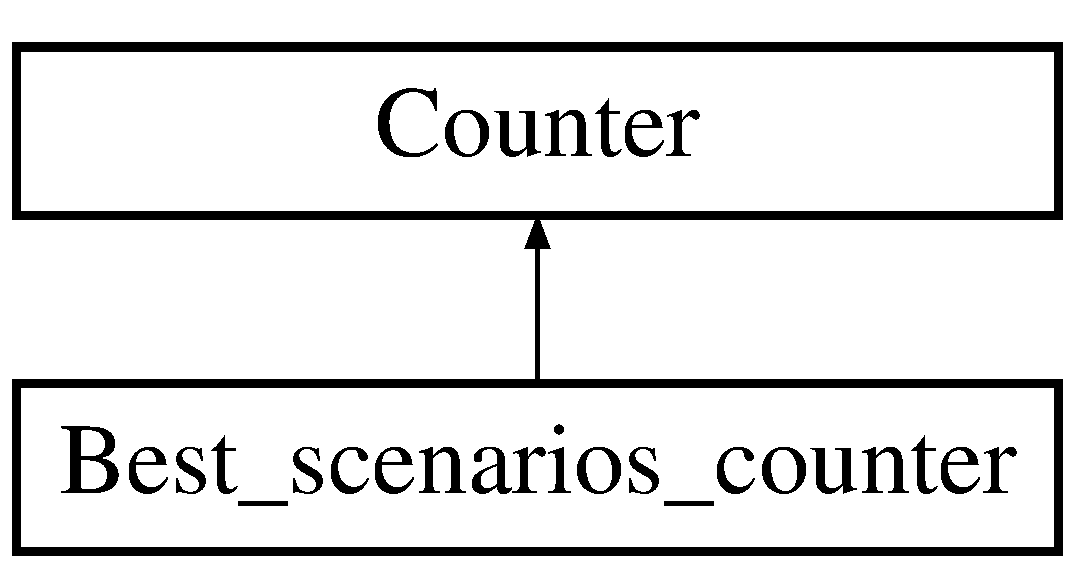
\includegraphics[height=2.000000cm]{d0/d7b/classBest__scenarios__counter}
\end{center}
\end{figure}
\subsection*{Public Member Functions}
\begin{DoxyCompactItemize}
\item 
\mbox{\Hypertarget{classBest__scenarios__counter_a1b02d09cb90d48901973a522879dbe11}\label{classBest__scenarios__counter_a1b02d09cb90d48901973a522879dbe11}} 
{\bfseries Best\+\_\+scenarios\+\_\+counter} (size\+\_\+t)
\item 
\mbox{\Hypertarget{classBest__scenarios__counter_a825bfa56893618db010d7bdd0a05fe11}\label{classBest__scenarios__counter_a825bfa56893618db010d7bdd0a05fe11}} 
{\bfseries Best\+\_\+scenarios\+\_\+counter} (size\+\_\+t, bool)
\item 
\mbox{\Hypertarget{classBest__scenarios__counter_a114a7eb723e63731f210436068ffa786}\label{classBest__scenarios__counter_a114a7eb723e63731f210436068ffa786}} 
{\bfseries Best\+\_\+scenarios\+\_\+counter} (size\+\_\+t, std\+::string)
\item 
\mbox{\Hypertarget{classBest__scenarios__counter_aabb594bc5fe34333cd31d4e33ddf7f3e}\label{classBest__scenarios__counter_aabb594bc5fe34333cd31d4e33ddf7f3e}} 
{\bfseries Best\+\_\+scenarios\+\_\+counter} (size\+\_\+t, std\+::string, bool)
\item 
\mbox{\Hypertarget{classBest__scenarios__counter_abb0a6a0997f579afb2ae3824a90ad2d0}\label{classBest__scenarios__counter_abb0a6a0997f579afb2ae3824a90ad2d0}} 
std\+::string {\bfseries type} () const
\item 
\mbox{\Hypertarget{classBest__scenarios__counter_ae5027552709dfc54fe972dfaae5e5a76}\label{classBest__scenarios__counter_ae5027552709dfc54fe972dfaae5e5a76}} 
void {\bfseries initialize\+\_\+counter} (const \hyperlink{classModel__Parms}{Model\+\_\+\+Parms} \&, const \hyperlink{classModel__marginals}{Model\+\_\+marginals} \&)
\item 
\mbox{\Hypertarget{classBest__scenarios__counter_ad5c78463063ea4223c489ca2e8678b31}\label{classBest__scenarios__counter_ad5c78463063ea4223c489ca2e8678b31}} 
void {\bfseries count\+\_\+scenario} (long double, double, const std\+::string \&, \hyperlink{classEnum__fast__memory__map}{Seq\+\_\+type\+\_\+str\+\_\+p\+\_\+map} \&, const \hyperlink{classEnum__fast__memory__dual__key__map}{Seq\+\_\+offsets\+\_\+map} \&, const std\+::unordered\+\_\+map$<$ std\+::tuple$<$ Event\+\_\+type, Gene\+\_\+class, Seq\+\_\+side $>$, std\+::shared\+\_\+ptr$<$ \hyperlink{classRec__Event}{Rec\+\_\+\+Event} $>$$>$ \&, \hyperlink{classEnum__fast__memory__map}{Mismatch\+\_\+vectors\+\_\+map} \&)
\item 
\mbox{\Hypertarget{classBest__scenarios__counter_a93d8eed7e5c5fafd7d9064492ac83a79}\label{classBest__scenarios__counter_a93d8eed7e5c5fafd7d9064492ac83a79}} 
void {\bfseries count\+\_\+sequence} (double, const \hyperlink{classModel__marginals}{Model\+\_\+marginals} \&, const \hyperlink{classModel__Parms}{Model\+\_\+\+Parms} \&)
\item 
\mbox{\Hypertarget{classBest__scenarios__counter_a860792c667b329c6877c3cc11b312488}\label{classBest__scenarios__counter_a860792c667b329c6877c3cc11b312488}} 
void {\bfseries add\+\_\+checked} (std\+::shared\+\_\+ptr$<$ \hyperlink{classCounter}{Counter} $>$)
\item 
\mbox{\Hypertarget{classBest__scenarios__counter_a9daf95a4846e7392cbf036c3aaf7cd73}\label{classBest__scenarios__counter_a9daf95a4846e7392cbf036c3aaf7cd73}} 
void {\bfseries dump\+\_\+sequence\+\_\+data} (int, int)
\item 
\mbox{\Hypertarget{classBest__scenarios__counter_af4457d69d9405e3ebd9c4ef359d40f57}\label{classBest__scenarios__counter_af4457d69d9405e3ebd9c4ef359d40f57}} 
std\+::shared\+\_\+ptr$<$ \hyperlink{classCounter}{Counter} $>$ {\bfseries copy} () const
\end{DoxyCompactItemize}
\subsection*{Public Attributes}
\begin{DoxyCompactItemize}
\item 
\mbox{\Hypertarget{classBest__scenarios__counter_abd0c0c2c1a2ac326b3897c7e9badad21}\label{classBest__scenarios__counter_abd0c0c2c1a2ac326b3897c7e9badad21}} 
size\+\_\+t {\bfseries n\+\_\+scenarios\+\_\+counted}
\item 
\mbox{\Hypertarget{classBest__scenarios__counter_a81323e4e4b6a1175da9370992297209a}\label{classBest__scenarios__counter_a81323e4e4b6a1175da9370992297209a}} 
std\+::shared\+\_\+ptr$<$ std\+::ofstream $>$ {\bfseries output\+\_\+scenario\+\_\+file\+\_\+ptr}
\item 
\mbox{\Hypertarget{classBest__scenarios__counter_abe8aa0d16e4fa62041df503a040e9428}\label{classBest__scenarios__counter_abe8aa0d16e4fa62041df503a040e9428}} 
std\+::queue$<$ std\+::vector$<$ int $>$ $>$ {\bfseries single\+\_\+scenario\+\_\+realizations\+\_\+queue}
\item 
\mbox{\Hypertarget{classBest__scenarios__counter_aaf1861459f6ef157ef87a3c53380d917}\label{classBest__scenarios__counter_aaf1861459f6ef157ef87a3c53380d917}} 
std\+::list$<$ int $>$ {\bfseries single\+\_\+scenario\+\_\+mismatches\+\_\+list}
\item 
\mbox{\Hypertarget{classBest__scenarios__counter_a6bb048e0cdacc5a6659a8c535c3c76fc}\label{classBest__scenarios__counter_a6bb048e0cdacc5a6659a8c535c3c76fc}} 
std\+::vector$<$ std\+::tuple$<$ double, std\+::queue$<$ std\+::vector$<$ int $>$ $>$, std\+::list$<$ int $>$ $>$ $>$ {\bfseries best\+\_\+scenarios\+\_\+vec}
\item 
\mbox{\Hypertarget{classBest__scenarios__counter_ab397a09b97161f3db1eb962759f4079d}\label{classBest__scenarios__counter_ab397a09b97161f3db1eb962759f4079d}} 
std\+::forward\+\_\+list$<$ std\+::shared\+\_\+ptr$<$ const \hyperlink{classRec__Event}{Rec\+\_\+\+Event} $>$ $>$ {\bfseries event\+\_\+fw\+\_\+list}
\end{DoxyCompactItemize}
\subsection*{Additional Inherited Members}


\subsection{Detailed Description}
Records the N best scenarios realizations and mismatches. 

\begin{DoxyAuthor}{Author}
Q.\+Marcou 
\end{DoxyAuthor}
\begin{DoxyVersion}{Version}
1.\+0
\end{DoxyVersion}
Implementation of the \hyperlink{classCounter}{Counter} abstract class. Records the N most likely scenario realizations and mismatches and append it to a semicolon separated file. 

The documentation for this class was generated from the following files\+:\begin{DoxyCompactItemize}
\item 
Bestscenarioscounter.\+h\item 
Bestscenarioscounter.\+cpp\end{DoxyCompactItemize}

\hypertarget{classCDR3SeqData}{}\section{C\+D\+R3\+Seq\+Data Class Reference}
\label{classCDR3SeqData}\index{C\+D\+R3\+Seq\+Data@{C\+D\+R3\+Seq\+Data}}


Class to store C\+D\+R3 information of a sequence.  




{\ttfamily \#include $<$C\+D\+R3\+Seq\+Data.\+h$>$}

\subsection*{Public Member Functions}
\begin{DoxyCompactItemize}
\item 
\mbox{\Hypertarget{classCDR3SeqData_a9e348ab1d83688bd91661ad12904f951}\label{classCDR3SeqData_a9e348ab1d83688bd91661ad12904f951}} 
{\bfseries C\+D\+R3\+Seq\+Data} (const \hyperlink{classCDR3SeqData}{C\+D\+R3\+Seq\+Data} \&orig)
\item 
\mbox{\Hypertarget{classCDR3SeqData_a96876a00149ba49cbcfafc79a0018aab}\label{classCDR3SeqData_a96876a00149ba49cbcfafc79a0018aab}} 
std\+::string {\bfseries str\+Data} ()
\end{DoxyCompactItemize}
\subsection*{Public Attributes}
\begin{DoxyCompactItemize}
\item 
\mbox{\Hypertarget{classCDR3SeqData_a7ba4d4e76a21c1db8cdb38564a8c46d4}\label{classCDR3SeqData_a7ba4d4e76a21c1db8cdb38564a8c46d4}} 
int {\bfseries seq\+\_\+index}
\item 
\mbox{\Hypertarget{classCDR3SeqData_aa31a3eda6390775b80e004711315e7ce}\label{classCDR3SeqData_aa31a3eda6390775b80e004711315e7ce}} 
int {\bfseries v\+\_\+anchor}
\item 
\mbox{\Hypertarget{classCDR3SeqData_a3c94df2f00900c5222cf4d6cee734de1}\label{classCDR3SeqData_a3c94df2f00900c5222cf4d6cee734de1}} 
int {\bfseries j\+\_\+anchor}
\item 
\mbox{\Hypertarget{classCDR3SeqData_a53d26a8a839509cb958280f1076de84b}\label{classCDR3SeqData_a53d26a8a839509cb958280f1076de84b}} 
std\+::string {\bfseries C\+D\+R3nt}
\item 
\mbox{\Hypertarget{classCDR3SeqData_ac7f039ed6d6ee402982e581211f1628d}\label{classCDR3SeqData_ac7f039ed6d6ee402982e581211f1628d}} 
std\+::string {\bfseries C\+D\+R3aa}
\end{DoxyCompactItemize}


\subsection{Detailed Description}
Class to store C\+D\+R3 information of a sequence. 

\begin{DoxyAuthor}{Author}
C. Olivares 
\end{DoxyAuthor}


The documentation for this class was generated from the following files\+:\begin{DoxyCompactItemize}
\item 
C\+D\+R3\+Seq\+Data.\+h\item 
C\+D\+R3\+Seq\+Data.\+cpp\end{DoxyCompactItemize}

\hypertarget{classCounter}{}\section{Counter Class Reference}
\label{classCounter}\index{Counter@{Counter}}


Scenario statistics recording abstract class.  




{\ttfamily \#include $<$Counter.\+h$>$}

Inheritance diagram for Counter\+:\begin{figure}[H]
\begin{center}
\leavevmode
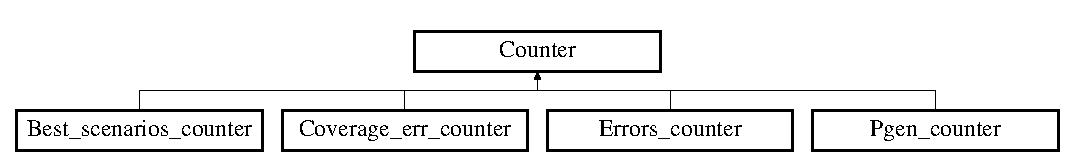
\includegraphics[height=1.794872cm]{d1/d24/classCounter}
\end{center}
\end{figure}
\subsection*{Public Member Functions}
\begin{DoxyCompactItemize}
\item 
\mbox{\Hypertarget{classCounter_a1ff0e754623c886cae1b76ab93a96faa}\label{classCounter_a1ff0e754623c886cae1b76ab93a96faa}} 
{\bfseries Counter} (const std\+::string \&path=\char`\"{}/tmp/\char`\"{}, bool last\+\_\+iter=false)
\item 
\mbox{\Hypertarget{classCounter_a13bbd01b9db02df144a4b303d0a8fc9a}\label{classCounter_a13bbd01b9db02df144a4b303d0a8fc9a}} 
virtual std\+::string {\bfseries type} () const =0
\item 
\mbox{\Hypertarget{classCounter_a56a86bc9430be6e0e9c8cf612b42a857}\label{classCounter_a56a86bc9430be6e0e9c8cf612b42a857}} 
virtual void {\bfseries initialize\+\_\+counter} (const \hyperlink{classModel__Parms}{Model\+\_\+\+Parms} \&, const \hyperlink{classModel__marginals}{Model\+\_\+marginals} \&)=0
\item 
\mbox{\Hypertarget{classCounter_a2aa0558b76714d3e5e11fee7dc310639}\label{classCounter_a2aa0558b76714d3e5e11fee7dc310639}} 
virtual void {\bfseries count\+\_\+scenario} (long double, double, const std\+::string \&, \hyperlink{classEnum__fast__memory__map}{Seq\+\_\+type\+\_\+str\+\_\+p\+\_\+map} \&, const \hyperlink{classEnum__fast__memory__dual__key__map}{Seq\+\_\+offsets\+\_\+map} \&, const std\+::unordered\+\_\+map$<$ std\+::tuple$<$ Event\+\_\+type, Gene\+\_\+class, Seq\+\_\+side $>$, std\+::shared\+\_\+ptr$<$ \hyperlink{classRec__Event}{Rec\+\_\+\+Event} $>$$>$ \&, \hyperlink{classEnum__fast__memory__map}{Mismatch\+\_\+vectors\+\_\+map} \&)
\item 
\mbox{\Hypertarget{classCounter_a2ceec8c6539b9912d1a6eb72a8a9d895}\label{classCounter_a2ceec8c6539b9912d1a6eb72a8a9d895}} 
virtual void {\bfseries count\+\_\+sequence} (double, const \hyperlink{classModel__marginals}{Model\+\_\+marginals} \&, const \hyperlink{classModel__Parms}{Model\+\_\+\+Parms} \&)
\item 
\mbox{\Hypertarget{classCounter_a1cbad4a20ed2bc666923c52f1f7de07c}\label{classCounter_a1cbad4a20ed2bc666923c52f1f7de07c}} 
virtual void {\bfseries add\+\_\+to\+\_\+counter} (std\+::shared\+\_\+ptr$<$ \hyperlink{classCounter}{Counter} $>$)
\item 
\mbox{\Hypertarget{classCounter_a108d1d8b84d1a4ec02e82d115bb090f0}\label{classCounter_a108d1d8b84d1a4ec02e82d115bb090f0}} 
virtual void {\bfseries add\+\_\+checked} (std\+::shared\+\_\+ptr$<$ \hyperlink{classCounter}{Counter} $>$)=0
\item 
\mbox{\Hypertarget{classCounter_a6d82f5fca039e761791d4e393ec3a75a}\label{classCounter_a6d82f5fca039e761791d4e393ec3a75a}} 
virtual void {\bfseries dump\+\_\+sequence\+\_\+data} (int, int)
\item 
\mbox{\Hypertarget{classCounter_a0bee773e60d141f7bf5d1dbd90d04c40}\label{classCounter_a0bee773e60d141f7bf5d1dbd90d04c40}} 
virtual void {\bfseries dump\+\_\+data\+\_\+summary} (int)
\item 
\mbox{\Hypertarget{classCounter_a6b04c1e240adf83cae0c85050d85355c}\label{classCounter_a6b04c1e240adf83cae0c85050d85355c}} 
bool {\bfseries is\+\_\+last\+\_\+iter\+\_\+only} () const
\item 
\mbox{\Hypertarget{classCounter_a19b291f7a6b19e93221bd73df296291f}\label{classCounter_a19b291f7a6b19e93221bd73df296291f}} 
std\+::string {\bfseries get\+\_\+path\+\_\+to\+\_\+files} () const
\item 
\mbox{\Hypertarget{classCounter_a2ec3d7154e44d3ef38a2c295eef53f26}\label{classCounter_a2ec3d7154e44d3ef38a2c295eef53f26}} 
void {\bfseries set\+\_\+path\+\_\+to\+\_\+files} (const std\+::string \&new\+\_\+path)
\item 
\mbox{\Hypertarget{classCounter_a1320d7111338de2b1764b09dc023f833}\label{classCounter_a1320d7111338de2b1764b09dc023f833}} 
virtual std\+::shared\+\_\+ptr$<$ \hyperlink{classCounter}{Counter} $>$ {\bfseries copy} () const =0
\end{DoxyCompactItemize}
\subsection*{Protected Attributes}
\begin{DoxyCompactItemize}
\item 
\mbox{\Hypertarget{classCounter_af15bb7f590112d08e29d194baf3e536e}\label{classCounter_af15bb7f590112d08e29d194baf3e536e}} 
std\+::string {\bfseries path\+\_\+to\+\_\+file}
\item 
\mbox{\Hypertarget{classCounter_aac0e458aae2f27e6a41570562087a347}\label{classCounter_aac0e458aae2f27e6a41570562087a347}} 
bool {\bfseries last\+\_\+iter\+\_\+only}
\item 
\mbox{\Hypertarget{classCounter_ac44c16637ced1d03608d10703bcaaccd}\label{classCounter_ac44c16637ced1d03608d10703bcaaccd}} 
bool {\bfseries fstreams\+\_\+created}
\end{DoxyCompactItemize}


\subsection{Detailed Description}
Scenario statistics recording abstract class. 

\begin{DoxyAuthor}{Author}
Q.\+Marcou 
\end{DoxyAuthor}
\begin{DoxyVersion}{Version}
1.\+0
\end{DoxyVersion}
The \hyperlink{classCounter}{Counter} abstract class provides an interface to collect individual scenarios statistics and aggregate them in various ways. 

The documentation for this class was generated from the following files\+:\begin{DoxyCompactItemize}
\item 
Counter.\+h\item 
Counter.\+cpp\end{DoxyCompactItemize}

\hypertarget{classCoverage__err__counter}{}\section{Coverage\+\_\+err\+\_\+counter Class Reference}
\label{classCoverage__err__counter}\index{Coverage\+\_\+err\+\_\+counter@{Coverage\+\_\+err\+\_\+counter}}


Records the number of time each genomic position is observed with or without error.  




{\ttfamily \#include $<$Coverageerrcounter.\+h$>$}

Inheritance diagram for Coverage\+\_\+err\+\_\+counter\+:\begin{figure}[H]
\begin{center}
\leavevmode
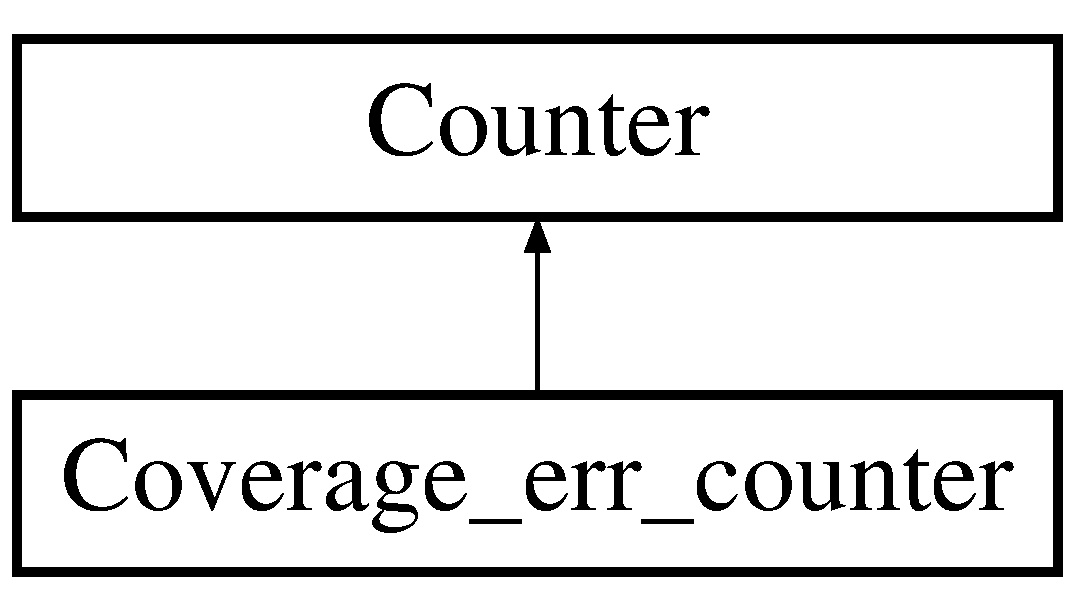
\includegraphics[height=2.000000cm]{d1/d51/classCoverage__err__counter}
\end{center}
\end{figure}
\subsection*{Public Member Functions}
\begin{DoxyCompactItemize}
\item 
\mbox{\Hypertarget{classCoverage__err__counter_a1744bf9764b432f500131439fd4afcfa}\label{classCoverage__err__counter_a1744bf9764b432f500131439fd4afcfa}} 
{\bfseries Coverage\+\_\+err\+\_\+counter} (Gene\+\_\+class)
\item 
\mbox{\Hypertarget{classCoverage__err__counter_a86f1b7a29bf0244cfd56e564329725e1}\label{classCoverage__err__counter_a86f1b7a29bf0244cfd56e564329725e1}} 
{\bfseries Coverage\+\_\+err\+\_\+counter} (Gene\+\_\+class, bool, bool)
\item 
\mbox{\Hypertarget{classCoverage__err__counter_a8d768e2bcf4c66d5b81c7cab85ac3701}\label{classCoverage__err__counter_a8d768e2bcf4c66d5b81c7cab85ac3701}} 
{\bfseries Coverage\+\_\+err\+\_\+counter} (std\+::string, Gene\+\_\+class, bool)
\item 
\mbox{\Hypertarget{classCoverage__err__counter_ab0c7dad32b9a61a83a3baf7f50fdab33}\label{classCoverage__err__counter_ab0c7dad32b9a61a83a3baf7f50fdab33}} 
{\bfseries Coverage\+\_\+err\+\_\+counter} (std\+::string, Gene\+\_\+class, size\+\_\+t, bool, bool)
\item 
\mbox{\Hypertarget{classCoverage__err__counter_afff8475b6327de18697e9d2068fb84b5}\label{classCoverage__err__counter_afff8475b6327de18697e9d2068fb84b5}} 
std\+::string {\bfseries type} () const
\item 
\mbox{\Hypertarget{classCoverage__err__counter_a333faaf6f622fa7cee77d34b226126d8}\label{classCoverage__err__counter_a333faaf6f622fa7cee77d34b226126d8}} 
void {\bfseries initialize\+\_\+counter} (const \hyperlink{classModel__Parms}{Model\+\_\+\+Parms} \&, const \hyperlink{classModel__marginals}{Model\+\_\+marginals} \&)
\item 
\mbox{\Hypertarget{classCoverage__err__counter_a6294a2c63795daeb6fea3506f27b19ac}\label{classCoverage__err__counter_a6294a2c63795daeb6fea3506f27b19ac}} 
void {\bfseries count\+\_\+scenario} (long double, double, const std\+::string \&, \hyperlink{classEnum__fast__memory__map}{Seq\+\_\+type\+\_\+str\+\_\+p\+\_\+map} \&, const \hyperlink{classEnum__fast__memory__dual__key__map}{Seq\+\_\+offsets\+\_\+map} \&, const std\+::unordered\+\_\+map$<$ std\+::tuple$<$ Event\+\_\+type, Gene\+\_\+class, Seq\+\_\+side $>$, std\+::shared\+\_\+ptr$<$ \hyperlink{classRec__Event}{Rec\+\_\+\+Event} $>$$>$ \&, \hyperlink{classEnum__fast__memory__map}{Mismatch\+\_\+vectors\+\_\+map} \&)
\item 
\mbox{\Hypertarget{classCoverage__err__counter_a20fde7a85141d52bd283583b0c12e030}\label{classCoverage__err__counter_a20fde7a85141d52bd283583b0c12e030}} 
void {\bfseries count\+\_\+sequence} (double, const \hyperlink{classModel__marginals}{Model\+\_\+marginals} \&, const \hyperlink{classModel__Parms}{Model\+\_\+\+Parms} \&)
\item 
\mbox{\Hypertarget{classCoverage__err__counter_a0d7a5ebfe75b5ff6ef5480b6a458abb2}\label{classCoverage__err__counter_a0d7a5ebfe75b5ff6ef5480b6a458abb2}} 
void {\bfseries add\+\_\+checked} (std\+::shared\+\_\+ptr$<$ \hyperlink{classCounter}{Counter} $>$)
\item 
\mbox{\Hypertarget{classCoverage__err__counter_addfe9e5441d62616022e1c0d2e6391b6}\label{classCoverage__err__counter_addfe9e5441d62616022e1c0d2e6391b6}} 
void {\bfseries dump\+\_\+sequence\+\_\+data} (int, int)
\item 
\mbox{\Hypertarget{classCoverage__err__counter_abafd7cd49e08c50b5d768eacc3ec7df3}\label{classCoverage__err__counter_abafd7cd49e08c50b5d768eacc3ec7df3}} 
void {\bfseries dump\+\_\+data\+\_\+summary} (int)
\item 
\mbox{\Hypertarget{classCoverage__err__counter_aa1b161227877e3cbb37fec90019ba906}\label{classCoverage__err__counter_aa1b161227877e3cbb37fec90019ba906}} 
std\+::shared\+\_\+ptr$<$ \hyperlink{classCounter}{Counter} $>$ {\bfseries copy} () const
\end{DoxyCompactItemize}
\subsection*{Additional Inherited Members}


\subsection{Detailed Description}
Records the number of time each genomic position is observed with or without error. 

\begin{DoxyAuthor}{Author}
Q.\+Marcou 
\end{DoxyAuthor}
\begin{DoxyVersion}{Version}
1.\+0
\end{DoxyVersion}
The \hyperlink{classCoverage__err__counter}{Coverage\+\_\+err\+\_\+counter} allows to record the number of times each genomic site is observed (coverage) and how many times a mismatch has been observed on it (error/mutation). The recording can be made at the single position level, as well as joint over positions duet,triplet etc (e.\+g the number of times two nucleotides were observed in the same scenario) 

The documentation for this class was generated from the following files\+:\begin{DoxyCompactItemize}
\item 
Coverageerrcounter.\+h\item 
Coverageerrcounter.\+cpp\end{DoxyCompactItemize}

\hypertarget{structD__position__comparator}{}\section{D\+\_\+position\+\_\+comparator Struct Reference}
\label{structD__position__comparator}\index{D\+\_\+position\+\_\+comparator@{D\+\_\+position\+\_\+comparator}}
\subsection*{Public Member Functions}
\begin{DoxyCompactItemize}
\item 
\mbox{\Hypertarget{structD__position__comparator_a5b97cf8744cccb01ae25947ceacfb5f5}\label{structD__position__comparator_a5b97cf8744cccb01ae25947ceacfb5f5}} 
bool {\bfseries operator()} (std\+::tuple$<$ std\+::string, int, int, double $>$ position\+\_\+1, std\+::tuple$<$ std\+::string, int, int, double $>$ position\+\_\+2)
\end{DoxyCompactItemize}


The documentation for this struct was generated from the following file\+:\begin{DoxyCompactItemize}
\item 
Utils.\+h\end{DoxyCompactItemize}

\hypertarget{classDeletion}{}\section{Deletion Class Reference}
\label{classDeletion}\index{Deletion@{Deletion}}


\hyperlink{classDeletion}{Deletion} recombination event.  




{\ttfamily \#include $<$Deletion.\+h$>$}

Inheritance diagram for Deletion\+:\begin{figure}[H]
\begin{center}
\leavevmode
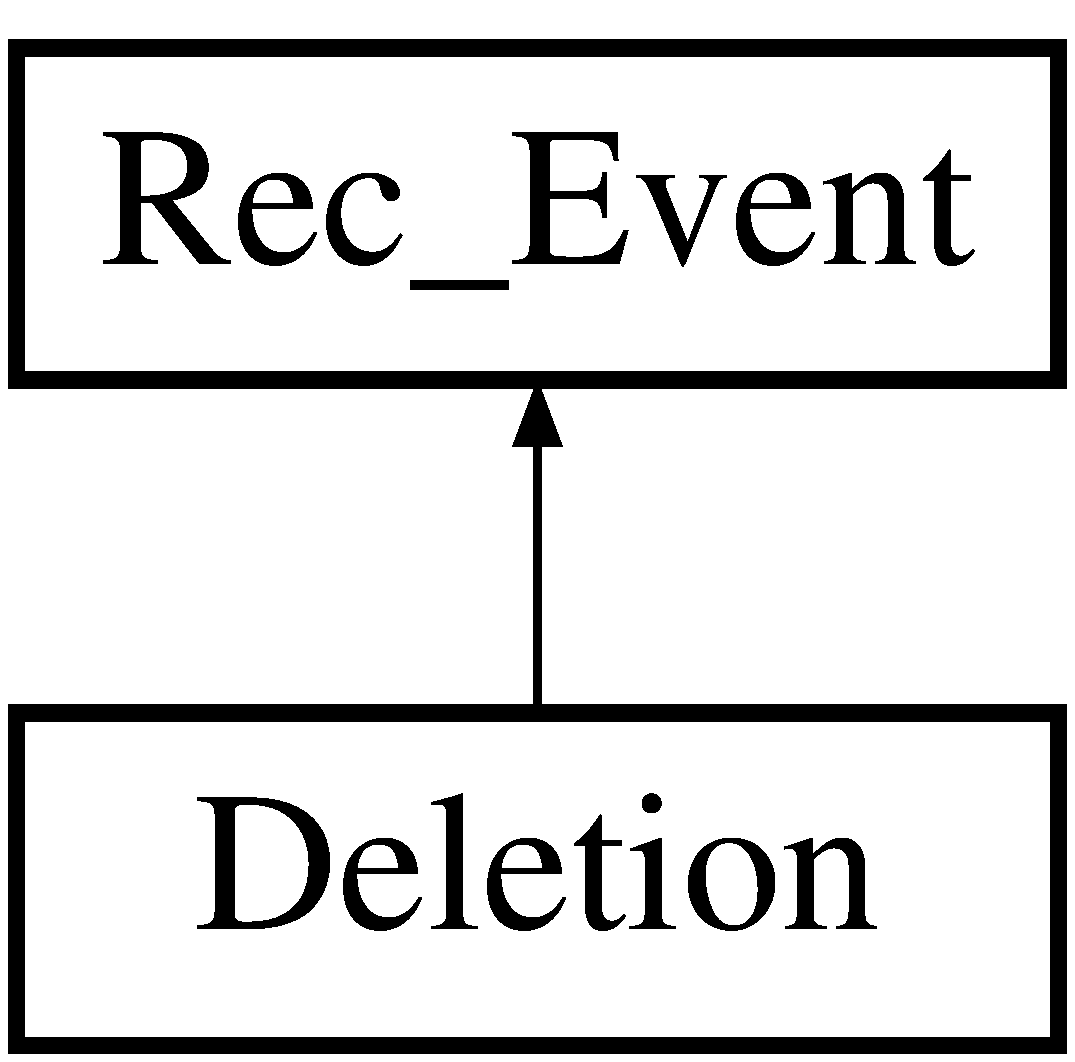
\includegraphics[height=2.000000cm]{d2/df0/classDeletion}
\end{center}
\end{figure}
\subsection*{Public Member Functions}
\begin{DoxyCompactItemize}
\item 
\mbox{\Hypertarget{classDeletion_a21f9224d32bb4b21eb8ca19a42d65b9b}\label{classDeletion_a21f9224d32bb4b21eb8ca19a42d65b9b}} 
{\bfseries Deletion} (Gene\+\_\+class, Seq\+\_\+side, std\+::pair$<$ int, int $>$)
\item 
\mbox{\Hypertarget{classDeletion_a494ec4114211df7bf0a7737510709d3c}\label{classDeletion_a494ec4114211df7bf0a7737510709d3c}} 
{\bfseries Deletion} (std\+::forward\+\_\+list$<$ int $>$)
\item 
\mbox{\Hypertarget{classDeletion_a9de4159829dc5435b8cd4dfc2962d303}\label{classDeletion_a9de4159829dc5435b8cd4dfc2962d303}} 
{\bfseries Deletion} (Gene\+\_\+class, Seq\+\_\+side)
\item 
\mbox{\Hypertarget{classDeletion_a794476abcfa448bb4f38d0f3666cc91d}\label{classDeletion_a794476abcfa448bb4f38d0f3666cc91d}} 
{\bfseries Deletion} (Gene\+\_\+class, Seq\+\_\+side, std\+::unordered\+\_\+map$<$ std\+::string, \hyperlink{structEvent__realization}{Event\+\_\+realization} $>$ \&)
\item 
\mbox{\Hypertarget{classDeletion_ae4e145381e8c4e51a66dd83f871d395a}\label{classDeletion_ae4e145381e8c4e51a66dd83f871d395a}} 
std\+::shared\+\_\+ptr$<$ \hyperlink{classRec__Event}{Rec\+\_\+\+Event} $>$ {\bfseries copy} ()
\item 
void \hyperlink{classDeletion_a2479968a06062e87027f8acef2631211}{iterate} (double \&, \hyperlink{classEnum__fast__memory__map}{Downstream\+\_\+scenario\+\_\+proba\+\_\+bound\+\_\+map} \&, const std\+::string \&, const \hyperlink{classInt__Str}{Int\+\_\+\+Str} \&, \hyperlink{classEnum__fast__memory__map}{Index\+\_\+map} \&, const std\+::unordered\+\_\+map$<$ Rec\+\_\+\+Event\+\_\+name, std\+::vector$<$ std\+::pair$<$ std\+::shared\+\_\+ptr$<$ const \hyperlink{classRec__Event}{Rec\+\_\+\+Event} $>$, int $>$$>$$>$ \&, std\+::shared\+\_\+ptr$<$ \hyperlink{classRec__Event}{Next\+\_\+event\+\_\+ptr} $>$ \&, Marginal\+\_\+array\+\_\+p \&, const Marginal\+\_\+array\+\_\+p \&, const std\+::unordered\+\_\+map$<$ Gene\+\_\+class, std\+::vector$<$ \hyperlink{structAlignment__data}{Alignment\+\_\+data} $>$$>$ \&, \hyperlink{classEnum__fast__memory__map}{Seq\+\_\+type\+\_\+str\+\_\+p\+\_\+map} \&, \hyperlink{classEnum__fast__memory__dual__key__map}{Seq\+\_\+offsets\+\_\+map} \&, std\+::shared\+\_\+ptr$<$ \hyperlink{classError__rate}{Error\+\_\+rate} $>$ \&, std\+::map$<$ size\+\_\+t, std\+::shared\+\_\+ptr$<$ \hyperlink{classCounter}{Counter} $>$$>$ \&, const std\+::unordered\+\_\+map$<$ std\+::tuple$<$ Event\+\_\+type, Gene\+\_\+class, Seq\+\_\+side $>$, std\+::shared\+\_\+ptr$<$ \hyperlink{classRec__Event}{Rec\+\_\+\+Event} $>$$>$ \&, \hyperlink{classEnum__fast__memory__map}{Safety\+\_\+bool\+\_\+map} \&, \hyperlink{classEnum__fast__memory__map}{Mismatch\+\_\+vectors\+\_\+map} \&, double \&, double \&)
\item 
\mbox{\Hypertarget{classDeletion_a6ae411d002a887a322b0a1ff7234cffc}\label{classDeletion_a6ae411d002a887a322b0a1ff7234cffc}} 
void {\bfseries add\+\_\+realization} (int)
\item 
\mbox{\Hypertarget{classDeletion_aec37ad3c8f6140f5e6968b3b0df0271a}\label{classDeletion_aec37ad3c8f6140f5e6968b3b0df0271a}} 
std\+::queue$<$ int $>$ {\bfseries draw\+\_\+random\+\_\+realization} (const Marginal\+\_\+array\+\_\+p \&, std\+::unordered\+\_\+map$<$ Rec\+\_\+\+Event\+\_\+name, int $>$ \&, const std\+::unordered\+\_\+map$<$ Rec\+\_\+\+Event\+\_\+name, std\+::vector$<$ std\+::pair$<$ std\+::shared\+\_\+ptr$<$ const \hyperlink{classRec__Event}{Rec\+\_\+\+Event} $>$, int $>$$>$$>$ \&, std\+::unordered\+\_\+map$<$ Seq\+\_\+type, std\+::string $>$ \&, std\+::mt19937\+\_\+64 \&) const
\item 
\mbox{\Hypertarget{classDeletion_a8e8dea0b2b7e8c1def855a758765b706}\label{classDeletion_a8e8dea0b2b7e8c1def855a758765b706}} 
void {\bfseries write2txt} (std\+::ofstream \&)
\item 
\mbox{\Hypertarget{classDeletion_aa4a0bb992b76d6a5984c26b3a70cb7be}\label{classDeletion_aa4a0bb992b76d6a5984c26b3a70cb7be}} 
void {\bfseries initialize\+\_\+event} (std\+::unordered\+\_\+set$<$ Rec\+\_\+\+Event\+\_\+name $>$ \&, const std\+::unordered\+\_\+map$<$ std\+::tuple$<$ Event\+\_\+type, Gene\+\_\+class, Seq\+\_\+side $>$, std\+::shared\+\_\+ptr$<$ \hyperlink{classRec__Event}{Rec\+\_\+\+Event} $>$$>$ \&, const std\+::unordered\+\_\+map$<$ Rec\+\_\+\+Event\+\_\+name, std\+::vector$<$ std\+::pair$<$ std\+::shared\+\_\+ptr$<$ const \hyperlink{classRec__Event}{Rec\+\_\+\+Event} $>$, int $>$$>$$>$ \&, \hyperlink{classEnum__fast__memory__map}{Downstream\+\_\+scenario\+\_\+proba\+\_\+bound\+\_\+map} \&, \hyperlink{classEnum__fast__memory__map}{Seq\+\_\+type\+\_\+str\+\_\+p\+\_\+map} \&, \hyperlink{classEnum__fast__memory__map}{Safety\+\_\+bool\+\_\+map} \&, std\+::shared\+\_\+ptr$<$ \hyperlink{classError__rate}{Error\+\_\+rate} $>$, \hyperlink{classEnum__fast__memory__map}{Mismatch\+\_\+vectors\+\_\+map} \&, \hyperlink{classEnum__fast__memory__dual__key__map}{Seq\+\_\+offsets\+\_\+map} \&, \hyperlink{classEnum__fast__memory__map}{Index\+\_\+map} \&)
\item 
\mbox{\Hypertarget{classDeletion_a2dee705a5c9b878dbccfef27c5305c7a}\label{classDeletion_a2dee705a5c9b878dbccfef27c5305c7a}} 
void {\bfseries add\+\_\+to\+\_\+marginals} (long double, Marginal\+\_\+array\+\_\+p \&) const
\item 
\mbox{\Hypertarget{classDeletion_a497f8a478a3c1065b11741b2bcadca0a}\label{classDeletion_a497f8a478a3c1065b11741b2bcadca0a}} 
bool {\bfseries has\+\_\+effect\+\_\+on} (Seq\+\_\+type) const
\item 
\mbox{\Hypertarget{classDeletion_aa28f61f8a3657da735d96ac007d61380}\label{classDeletion_aa28f61f8a3657da735d96ac007d61380}} 
void {\bfseries iterate\+\_\+initialize\+\_\+\+Len\+\_\+proba} (Seq\+\_\+type considered\+\_\+junction, std\+::map$<$ int, double $>$ \&length\+\_\+best\+\_\+proba\+\_\+map, std\+::queue$<$ std\+::shared\+\_\+ptr$<$ \hyperlink{classRec__Event}{Rec\+\_\+\+Event} $>$$>$ \&model\+\_\+queue, double \&scenario\+\_\+proba, const Marginal\+\_\+array\+\_\+p \&model\+\_\+parameters\+\_\+point, \hyperlink{classEnum__fast__memory__map}{Index\+\_\+map} \&base\+\_\+index\+\_\+map, \hyperlink{classEnum__fast__memory__map}{Seq\+\_\+type\+\_\+str\+\_\+p\+\_\+map} \&constructed\+\_\+sequences, int \&seq\+\_\+len) const
\item 
\mbox{\Hypertarget{classDeletion_a8439fb5c579245ea6038578fcfae0c86}\label{classDeletion_a8439fb5c579245ea6038578fcfae0c86}} 
void {\bfseries initialize\+\_\+\+Len\+\_\+proba\+\_\+bound} (std\+::queue$<$ std\+::shared\+\_\+ptr$<$ \hyperlink{classRec__Event}{Rec\+\_\+\+Event} $>$$>$ \&model\+\_\+queue, const Marginal\+\_\+array\+\_\+p \&model\+\_\+parameters\+\_\+point, \hyperlink{classEnum__fast__memory__map}{Index\+\_\+map} \&base\+\_\+index\+\_\+map)
\end{DoxyCompactItemize}
\subsection*{Friends}
\begin{DoxyCompactItemize}
\item 
\mbox{\Hypertarget{classDeletion_ad4a26da5a0e142c5135c983af6d042d6}\label{classDeletion_ad4a26da5a0e142c5135c983af6d042d6}} 
class {\bfseries Coverage\+\_\+err\+\_\+counter}
\item 
\mbox{\Hypertarget{classDeletion_ad5a47907bf54eec60bc584c426aaca7f}\label{classDeletion_ad5a47907bf54eec60bc584c426aaca7f}} 
class {\bfseries Hypermutation\+\_\+global\+\_\+errorrate}
\item 
\mbox{\Hypertarget{classDeletion_a5ff5d89d255ca8ca355c6da8c4be7f68}\label{classDeletion_a5ff5d89d255ca8ca355c6da8c4be7f68}} 
class {\bfseries Hypermutation\+\_\+full\+\_\+\+Nmer\+\_\+errorrate}
\end{DoxyCompactItemize}
\subsection*{Additional Inherited Members}


\subsection{Detailed Description}
\hyperlink{classDeletion}{Deletion} recombination event. 

\begin{DoxyAuthor}{Author}
Q.\+Marcou 
\end{DoxyAuthor}
\begin{DoxyVersion}{Version}
1.\+0
\end{DoxyVersion}
The \hyperlink{classDeletion}{Deletion} Rec\+Event models deletions of one genomic fragment on a given side. Deletions can be either positive or negative (= Palindromic insertions)

By construction the corresponding Gene\+Choice must have been explored first. 

\subsection{Member Function Documentation}
\mbox{\Hypertarget{classDeletion_a2479968a06062e87027f8acef2631211}\label{classDeletion_a2479968a06062e87027f8acef2631211}} 
\index{Deletion@{Deletion}!iterate@{iterate}}
\index{iterate@{iterate}!Deletion@{Deletion}}
\subsubsection{\texorpdfstring{iterate()}{iterate()}}
{\footnotesize\ttfamily void Deletion\+::iterate (\begin{DoxyParamCaption}\item[{double \&}]{,  }\item[{\hyperlink{classEnum__fast__memory__map}{Downstream\+\_\+scenario\+\_\+proba\+\_\+bound\+\_\+map} \&}]{,  }\item[{const std\+::string \&}]{,  }\item[{const \hyperlink{classInt__Str}{Int\+\_\+\+Str} \&}]{,  }\item[{\hyperlink{classEnum__fast__memory__map}{Index\+\_\+map} \&}]{,  }\item[{const std\+::unordered\+\_\+map$<$ Rec\+\_\+\+Event\+\_\+name, std\+::vector$<$ std\+::pair$<$ std\+::shared\+\_\+ptr$<$ const \hyperlink{classRec__Event}{Rec\+\_\+\+Event} $>$, int $>$$>$$>$ \&}]{,  }\item[{std\+::shared\+\_\+ptr$<$ \hyperlink{classRec__Event}{Next\+\_\+event\+\_\+ptr} $>$ \&}]{,  }\item[{Marginal\+\_\+array\+\_\+p \&}]{,  }\item[{const Marginal\+\_\+array\+\_\+p \&}]{,  }\item[{const std\+::unordered\+\_\+map$<$ Gene\+\_\+class, std\+::vector$<$ \hyperlink{structAlignment__data}{Alignment\+\_\+data} $>$$>$ \&}]{,  }\item[{\hyperlink{classEnum__fast__memory__map}{Seq\+\_\+type\+\_\+str\+\_\+p\+\_\+map} \&}]{,  }\item[{\hyperlink{classEnum__fast__memory__dual__key__map}{Seq\+\_\+offsets\+\_\+map} \&}]{,  }\item[{std\+::shared\+\_\+ptr$<$ \hyperlink{classError__rate}{Error\+\_\+rate} $>$ \&}]{,  }\item[{std\+::map$<$ size\+\_\+t, std\+::shared\+\_\+ptr$<$ \hyperlink{classCounter}{Counter} $>$$>$ \&}]{,  }\item[{const std\+::unordered\+\_\+map$<$ std\+::tuple$<$ Event\+\_\+type, Gene\+\_\+class, Seq\+\_\+side $>$, std\+::shared\+\_\+ptr$<$ \hyperlink{classRec__Event}{Rec\+\_\+\+Event} $>$$>$ \&}]{,  }\item[{\hyperlink{classEnum__fast__memory__map}{Safety\+\_\+bool\+\_\+map} \&}]{,  }\item[{\hyperlink{classEnum__fast__memory__map}{Mismatch\+\_\+vectors\+\_\+map} \&}]{,  }\item[{double \&}]{,  }\item[{double \&}]{ }\end{DoxyParamCaption})\hspace{0.3cm}{\ttfamily [inline]}, {\ttfamily [virtual]}}

General\+: Loop over all possible number of deletions for a given gene on a given sequence side

Specific\+: -\/\+First check whether any of these number of deletions is possible given the current position and number of deletions on other genes -\/\+Loop over \# of deletions in decreasing order T\+H\+IS IS A T\+E\+M\+P\+O\+R\+A\+RY F\+I\+X// //\+F\+I\+X\+ME

T\+H\+IS IS A T\+E\+M\+P\+O\+R\+A\+RY F\+I\+X// //\+F\+I\+X\+ME

T\+H\+IS IS A T\+E\+M\+P\+O\+R\+A\+RY F\+I\+X// //\+F\+I\+X\+ME

Implements \hyperlink{classRec__Event_a0fea607ec06bdd1a7f5ebb04a96e5253}{Rec\+\_\+\+Event}.



The documentation for this class was generated from the following files\+:\begin{DoxyCompactItemize}
\item 
Deletion.\+h\item 
Deletion.\+cpp\end{DoxyCompactItemize}

\hypertarget{classDinucl__markov}{}\section{Dinucl\+\_\+markov Class Reference}
\label{classDinucl__markov}\index{Dinucl\+\_\+markov@{Dinucl\+\_\+markov}}


Dinucleotide insertion Markov model.  


Inheritance diagram for Dinucl\+\_\+markov\+:\begin{figure}[H]
\begin{center}
\leavevmode
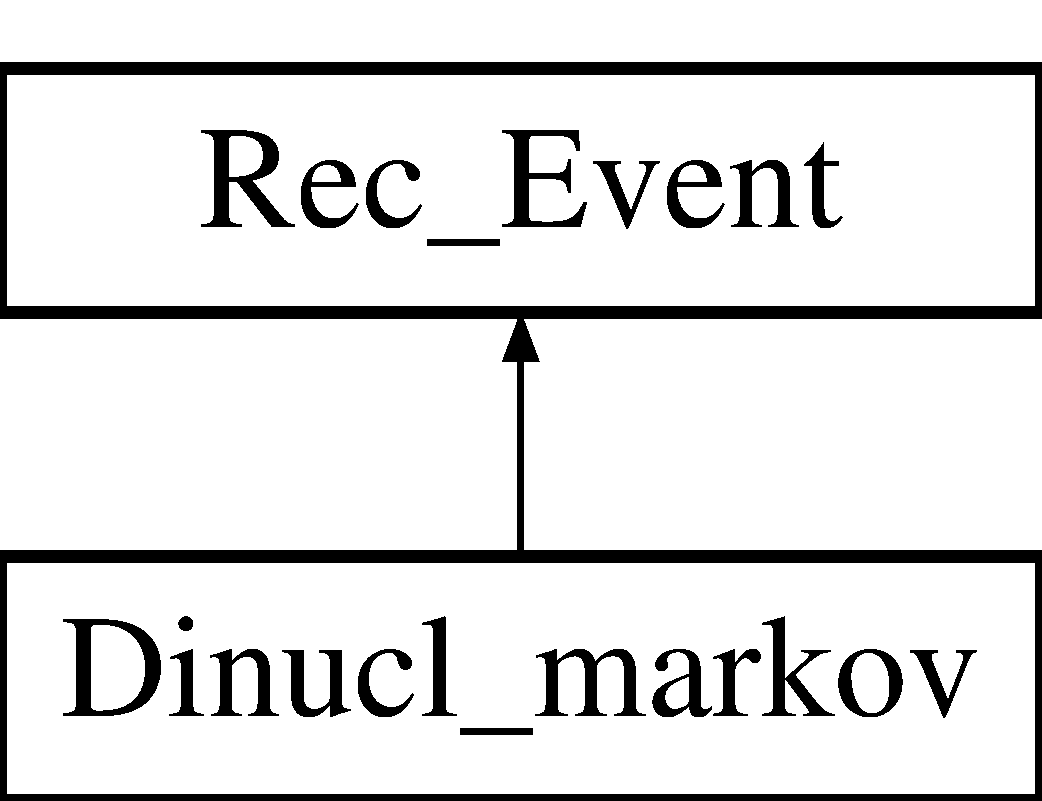
\includegraphics[height=2.000000cm]{d0/d2a/classDinucl__markov}
\end{center}
\end{figure}
\subsection*{Public Member Functions}
\begin{DoxyCompactItemize}
\item 
\mbox{\Hypertarget{classDinucl__markov_a7c4b9c77a45d66a4bb540a12cc75073a}\label{classDinucl__markov_a7c4b9c77a45d66a4bb540a12cc75073a}} 
{\bfseries Dinucl\+\_\+markov} (Gene\+\_\+class)
\item 
\mbox{\Hypertarget{classDinucl__markov_aef20fac2861787b1f03143dbd4a8224d}\label{classDinucl__markov_aef20fac2861787b1f03143dbd4a8224d}} 
std\+::shared\+\_\+ptr$<$ \hyperlink{classRec__Event}{Rec\+\_\+\+Event} $>$ {\bfseries copy} ()
\item 
\mbox{\Hypertarget{classDinucl__markov_a5080c4cf4545622858c5afb7c3130fa9}\label{classDinucl__markov_a5080c4cf4545622858c5afb7c3130fa9}} 
int {\bfseries size} () const
\item 
void \hyperlink{classDinucl__markov_ace49d0da113be7d77ad0d4c3b8152c3d}{iterate} (double \&, \hyperlink{classEnum__fast__memory__map}{Downstream\+\_\+scenario\+\_\+proba\+\_\+bound\+\_\+map} \&, const std\+::string \&, const \hyperlink{classInt__Str}{Int\+\_\+\+Str} \&, \hyperlink{classEnum__fast__memory__map}{Index\+\_\+map} \&, const std\+::unordered\+\_\+map$<$ Rec\+\_\+\+Event\+\_\+name, std\+::vector$<$ std\+::pair$<$ std\+::shared\+\_\+ptr$<$ const \hyperlink{classRec__Event}{Rec\+\_\+\+Event} $>$, int $>$$>$$>$ \&, std\+::shared\+\_\+ptr$<$ \hyperlink{classRec__Event}{Next\+\_\+event\+\_\+ptr} $>$ \&, Marginal\+\_\+array\+\_\+p \&, const Marginal\+\_\+array\+\_\+p \&, const std\+::unordered\+\_\+map$<$ Gene\+\_\+class, std\+::vector$<$ \hyperlink{structAlignment__data}{Alignment\+\_\+data} $>$$>$ \&, \hyperlink{classEnum__fast__memory__map}{Seq\+\_\+type\+\_\+str\+\_\+p\+\_\+map} \&, \hyperlink{classEnum__fast__memory__dual__key__map}{Seq\+\_\+offsets\+\_\+map} \&, std\+::shared\+\_\+ptr$<$ \hyperlink{classError__rate}{Error\+\_\+rate} $>$ \&, std\+::map$<$ size\+\_\+t, std\+::shared\+\_\+ptr$<$ \hyperlink{classCounter}{Counter} $>$$>$ \&, const std\+::unordered\+\_\+map$<$ std\+::tuple$<$ Event\+\_\+type, Gene\+\_\+class, Seq\+\_\+side $>$, std\+::shared\+\_\+ptr$<$ \hyperlink{classRec__Event}{Rec\+\_\+\+Event} $>$$>$ \&, \hyperlink{classEnum__fast__memory__map}{Safety\+\_\+bool\+\_\+map} \&, \hyperlink{classEnum__fast__memory__map}{Mismatch\+\_\+vectors\+\_\+map} \&, double \&, double \&)
\begin{DoxyCompactList}\small\item\em Evaluate all Event\+\_\+\+Realization of a Rec\+Event for a given sequence. \end{DoxyCompactList}\item 
\mbox{\Hypertarget{classDinucl__markov_aaeb38e8ed71cd1faaf6dfdbbf621d200}\label{classDinucl__markov_aaeb38e8ed71cd1faaf6dfdbbf621d200}} 
void {\bfseries add\+\_\+realization} (int)
\item 
\mbox{\Hypertarget{classDinucl__markov_a8b15545357ac34b0adc7c142036238df}\label{classDinucl__markov_a8b15545357ac34b0adc7c142036238df}} 
std\+::queue$<$ int $>$ {\bfseries draw\+\_\+random\+\_\+realization} (const Marginal\+\_\+array\+\_\+p \&, std\+::unordered\+\_\+map$<$ Rec\+\_\+\+Event\+\_\+name, int $>$ \&, const std\+::unordered\+\_\+map$<$ Rec\+\_\+\+Event\+\_\+name, std\+::vector$<$ std\+::pair$<$ std\+::shared\+\_\+ptr$<$ const \hyperlink{classRec__Event}{Rec\+\_\+\+Event} $>$, int $>$$>$$>$ \&, std\+::unordered\+\_\+map$<$ Seq\+\_\+type, std\+::string $>$ \&, std\+::mt19937\+\_\+64 \&) const
\item 
\mbox{\Hypertarget{classDinucl__markov_a911fd57910ede07e9f41a0be488f3366}\label{classDinucl__markov_a911fd57910ede07e9f41a0be488f3366}} 
void {\bfseries write2txt} (std\+::ofstream \&)
\item 
\mbox{\Hypertarget{classDinucl__markov_a1992380f533087999d03c3cb8bd05e72}\label{classDinucl__markov_a1992380f533087999d03c3cb8bd05e72}} 
void {\bfseries ind\+\_\+normalize} (Marginal\+\_\+array\+\_\+p \&, size\+\_\+t) const
\item 
\mbox{\Hypertarget{classDinucl__markov_a8373decc16c87577a47711bc20fb41bc}\label{classDinucl__markov_a8373decc16c87577a47711bc20fb41bc}} 
void {\bfseries initialize\+\_\+event} (std\+::unordered\+\_\+set$<$ Rec\+\_\+\+Event\+\_\+name $>$ \&, const std\+::unordered\+\_\+map$<$ std\+::tuple$<$ Event\+\_\+type, Gene\+\_\+class, Seq\+\_\+side $>$, std\+::shared\+\_\+ptr$<$ \hyperlink{classRec__Event}{Rec\+\_\+\+Event} $>$$>$ \&, const std\+::unordered\+\_\+map$<$ Rec\+\_\+\+Event\+\_\+name, std\+::vector$<$ std\+::pair$<$ std\+::shared\+\_\+ptr$<$ const \hyperlink{classRec__Event}{Rec\+\_\+\+Event} $>$, int $>$$>$$>$ \&, \hyperlink{classEnum__fast__memory__map}{Downstream\+\_\+scenario\+\_\+proba\+\_\+bound\+\_\+map} \&, \hyperlink{classEnum__fast__memory__map}{Seq\+\_\+type\+\_\+str\+\_\+p\+\_\+map} \&, \hyperlink{classEnum__fast__memory__map}{Safety\+\_\+bool\+\_\+map} \&, std\+::shared\+\_\+ptr$<$ \hyperlink{classError__rate}{Error\+\_\+rate} $>$, \hyperlink{classEnum__fast__memory__map}{Mismatch\+\_\+vectors\+\_\+map} \&, \hyperlink{classEnum__fast__memory__dual__key__map}{Seq\+\_\+offsets\+\_\+map} \&, \hyperlink{classEnum__fast__memory__map}{Index\+\_\+map} \&)
\item 
void \hyperlink{classDinucl__markov_a63fd37e31c3e32fee54dc26146bc3fac}{add\+\_\+to\+\_\+marginals} (long double, Marginal\+\_\+array\+\_\+p \&) const
\item 
void \hyperlink{classDinucl__markov_a8da33acb0a389a0a4c845a69c11b173c}{update\+\_\+event\+\_\+internal\+\_\+probas} (const Marginal\+\_\+array\+\_\+p \&, const std\+::unordered\+\_\+map$<$ Rec\+\_\+\+Event\+\_\+name, int $>$ \&)
\item 
\mbox{\Hypertarget{classDinucl__markov_ad19e4458a31477f56f18150e7ea3f731}\label{classDinucl__markov_ad19e4458a31477f56f18150e7ea3f731}} 
double $\ast$ {\bfseries get\+\_\+updated\+\_\+ptr} ()
\item 
\mbox{\Hypertarget{classDinucl__markov_a146a953912fbdd13dda74693b2972981}\label{classDinucl__markov_a146a953912fbdd13dda74693b2972981}} 
void {\bfseries initialize\+\_\+crude\+\_\+scenario\+\_\+proba\+\_\+bound} (double \&, std\+::forward\+\_\+list$<$ double $\ast$$>$ \&, const std\+::unordered\+\_\+map$<$ std\+::tuple$<$ Event\+\_\+type, Gene\+\_\+class, Seq\+\_\+side $>$, std\+::shared\+\_\+ptr$<$ \hyperlink{classRec__Event}{Rec\+\_\+\+Event} $>$$>$ \&)
\item 
\mbox{\Hypertarget{classDinucl__markov_a00c9b729b4984421c444f9543d241f6c}\label{classDinucl__markov_a00c9b729b4984421c444f9543d241f6c}} 
bool {\bfseries has\+\_\+effect\+\_\+on} (Seq\+\_\+type) const
\item 
\mbox{\Hypertarget{classDinucl__markov_a93c1b5d8073d5456419e87452f800027}\label{classDinucl__markov_a93c1b5d8073d5456419e87452f800027}} 
void {\bfseries iterate\+\_\+initialize\+\_\+\+Len\+\_\+proba} (Seq\+\_\+type considered\+\_\+junction, std\+::map$<$ int, double $>$ \&length\+\_\+best\+\_\+proba\+\_\+map, std\+::queue$<$ std\+::shared\+\_\+ptr$<$ \hyperlink{classRec__Event}{Rec\+\_\+\+Event} $>$$>$ \&model\+\_\+queue, double \&scenario\+\_\+proba, const Marginal\+\_\+array\+\_\+p \&model\+\_\+parameters\+\_\+point, \hyperlink{classEnum__fast__memory__map}{Index\+\_\+map} \&base\+\_\+index\+\_\+map, \hyperlink{classEnum__fast__memory__map}{Seq\+\_\+type\+\_\+str\+\_\+p\+\_\+map} \&constructed\+\_\+sequences, int \&seq\+\_\+len) const
\item 
\mbox{\Hypertarget{classDinucl__markov_a7fc4210d8943892078c6eeec7ddcfbd8}\label{classDinucl__markov_a7fc4210d8943892078c6eeec7ddcfbd8}} 
void {\bfseries initialize\+\_\+\+Len\+\_\+proba\+\_\+bound} (std\+::queue$<$ std\+::shared\+\_\+ptr$<$ \hyperlink{classRec__Event}{Rec\+\_\+\+Event} $>$$>$ \&model\+\_\+queue, const Marginal\+\_\+array\+\_\+p \&model\+\_\+parameters\+\_\+point, \hyperlink{classEnum__fast__memory__map}{Index\+\_\+map} \&base\+\_\+index\+\_\+map)
\end{DoxyCompactItemize}
\subsection*{Additional Inherited Members}


\subsection{Detailed Description}
Dinucleotide insertion Markov model. 

\begin{DoxyAuthor}{Author}
Q.\+Marcou 
\end{DoxyAuthor}
\begin{DoxyVersion}{Version}
1.\+0
\end{DoxyVersion}
Models a Markov chain dictating the identity of inserted nucleotides in the inserted region. We assume a low error frequency and almost flat dinucleotide model regime such that we use an euristic to extract the most likely realization. This choice has been made because the full handling through a forward algorithm would not be able to cope with e.\+g context dependent errors.

By construction the \hyperlink{classInsertion}{Insertion} event must have been explored first 

\subsection{Member Function Documentation}
\mbox{\Hypertarget{classDinucl__markov_a63fd37e31c3e32fee54dc26146bc3fac}\label{classDinucl__markov_a63fd37e31c3e32fee54dc26146bc3fac}} 
\index{Dinucl\+\_\+markov@{Dinucl\+\_\+markov}!add\+\_\+to\+\_\+marginals@{add\+\_\+to\+\_\+marginals}}
\index{add\+\_\+to\+\_\+marginals@{add\+\_\+to\+\_\+marginals}!Dinucl\+\_\+markov@{Dinucl\+\_\+markov}}
\subsubsection{\texorpdfstring{add\+\_\+to\+\_\+marginals()}{add\_to\_marginals()}}
{\footnotesize\ttfamily void Dinucl\+\_\+markov\+::add\+\_\+to\+\_\+marginals (\begin{DoxyParamCaption}\item[{long double}]{scenario\+\_\+proba,  }\item[{Marginal\+\_\+array\+\_\+p \&}]{updated\+\_\+marginals }\end{DoxyParamCaption}) const\hspace{0.3cm}{\ttfamily [virtual]}}

\begin{DoxyRefDesc}{Bug}
\item[\hyperlink{bug__bug000002}{Bug}]Will only count realizations of unambiguous nucleotides (realization indices$>$=0 since they are set to -\/1 in iterate\+\_\+common) \end{DoxyRefDesc}


Implements \hyperlink{classRec__Event}{Rec\+\_\+\+Event}.

\mbox{\Hypertarget{classDinucl__markov_ace49d0da113be7d77ad0d4c3b8152c3d}\label{classDinucl__markov_ace49d0da113be7d77ad0d4c3b8152c3d}} 
\index{Dinucl\+\_\+markov@{Dinucl\+\_\+markov}!iterate@{iterate}}
\index{iterate@{iterate}!Dinucl\+\_\+markov@{Dinucl\+\_\+markov}}
\subsubsection{\texorpdfstring{iterate()}{iterate()}}
{\footnotesize\ttfamily void Dinucl\+\_\+markov\+::iterate (\begin{DoxyParamCaption}\item[{double \&}]{,  }\item[{\hyperlink{classEnum__fast__memory__map}{Downstream\+\_\+scenario\+\_\+proba\+\_\+bound\+\_\+map} \&}]{,  }\item[{const std\+::string \&}]{,  }\item[{const \hyperlink{classInt__Str}{Int\+\_\+\+Str} \&}]{,  }\item[{\hyperlink{classEnum__fast__memory__map}{Index\+\_\+map} \&}]{,  }\item[{const std\+::unordered\+\_\+map$<$ Rec\+\_\+\+Event\+\_\+name, std\+::vector$<$ std\+::pair$<$ std\+::shared\+\_\+ptr$<$ const \hyperlink{classRec__Event}{Rec\+\_\+\+Event} $>$, int $>$$>$$>$ \&}]{,  }\item[{std\+::shared\+\_\+ptr$<$ \hyperlink{classRec__Event}{Next\+\_\+event\+\_\+ptr} $>$ \&}]{,  }\item[{Marginal\+\_\+array\+\_\+p \&}]{,  }\item[{const Marginal\+\_\+array\+\_\+p \&}]{,  }\item[{const std\+::unordered\+\_\+map$<$ Gene\+\_\+class, std\+::vector$<$ \hyperlink{structAlignment__data}{Alignment\+\_\+data} $>$$>$ \&}]{,  }\item[{\hyperlink{classEnum__fast__memory__map}{Seq\+\_\+type\+\_\+str\+\_\+p\+\_\+map} \&}]{,  }\item[{\hyperlink{classEnum__fast__memory__dual__key__map}{Seq\+\_\+offsets\+\_\+map} \&}]{,  }\item[{std\+::shared\+\_\+ptr$<$ \hyperlink{classError__rate}{Error\+\_\+rate} $>$ \&}]{,  }\item[{std\+::map$<$ size\+\_\+t, std\+::shared\+\_\+ptr$<$ \hyperlink{classCounter}{Counter} $>$$>$ \&}]{,  }\item[{const std\+::unordered\+\_\+map$<$ std\+::tuple$<$ Event\+\_\+type, Gene\+\_\+class, Seq\+\_\+side $>$, std\+::shared\+\_\+ptr$<$ \hyperlink{classRec__Event}{Rec\+\_\+\+Event} $>$$>$ \&}]{,  }\item[{\hyperlink{classEnum__fast__memory__map}{Safety\+\_\+bool\+\_\+map} \&}]{,  }\item[{\hyperlink{classEnum__fast__memory__map}{Mismatch\+\_\+vectors\+\_\+map} \&}]{,  }\item[{double \&}]{,  }\item[{double \&}]{ }\end{DoxyParamCaption})\hspace{0.3cm}{\ttfamily [inline]}, {\ttfamily [virtual]}}



Evaluate all Event\+\_\+\+Realization of a Rec\+Event for a given sequence. 

\begin{DoxyAuthor}{Author}
Q.\+Marcou 
\end{DoxyAuthor}
\begin{DoxyVersion}{Version}
1.\+0 
\end{DoxyVersion}

\begin{DoxyParams}[1]{Parameters}
\mbox{\tt in,out}  & {\em scenario\+\_\+proba} & Probability of the currently explored (incomplete) scenario \\
\hline
\mbox{\tt in,out}  & {\em downstream\+\_\+proba\+\_\+map} & \\
\hline
\mbox{\tt in}  & {\em sequence} & The studied sequence in nucleotide code \\
\hline
\mbox{\tt in}  & {\em int\+\_\+sequence} & The studied sequence in integer code \\
\hline
\mbox{\tt in,out}  & {\em base\+\_\+index\+\_\+map} & Dynamic map recording where probabilities should be read on the marginals. \\
\hline
\mbox{\tt in}  & {\em offset\+\_\+map} & Tells the event by how much indices from the children events should be modified \\
\hline
\mbox{\tt in}  & {\em next\+\_\+event\+\_\+ptr\+\_\+arr} & Indicates the next event to call iterate on \\
\hline
\mbox{\tt in}  & {\em updated\+\_\+marginals\+\_\+point} & Summary marginals on which complete scenario posteriors are recorded \\
\hline
\mbox{\tt in}  & {\em model\+\_\+parameters\+\_\+point} & Current recombination probability distribution \\
\hline
\mbox{\tt in}  & {\em allowed\+\_\+realizations} & The set of genomic templates alignment \\
\hline
\mbox{\tt in,out}  & {\em constructed\+\_\+sequences} & Map containing the (incomplete) scenario\textquotesingle{}s resulting sequence \\
\hline
\mbox{\tt in,out}  & {\em seq\+\_\+offsets} & Map containing the 3\textquotesingle{} and 5\textquotesingle{} offsets of each scenario sequence piece \\
\hline
\mbox{\tt in}  & {\em error\+\_\+rate\+\_\+p} & Pointer to the error model object \\
\hline
\mbox{\tt in}  & {\em counters\+\_\+list} & The list of \hyperlink{classCounter}{Counter} to be counted \\
\hline
\mbox{\tt in}  & {\em events\+\_\+map} & A map containing all events contained in the Model\+\_\+parms, accessible through their type, gene class and side. \\
\hline
\mbox{\tt in,out}  & {\em safety\+\_\+set} & A map indicating whether checks on offsets overlap should be performed \\
\hline
\mbox{\tt in,out}  & {\em mismatches\+\_\+lists} & A map containing the (incomplete) scenario mismatches \\
\hline
\mbox{\tt in}  & {\em seq\+\_\+max\+\_\+prob\+\_\+scenario} & Most likely scenario\textquotesingle{}s probability for the considered sequence \\
\hline
\mbox{\tt in}  & {\em proba\+\_\+threshold\+\_\+factor} & Threshold on probability ratio between most likely scenario and explored scenario\\
\hline
\end{DoxyParams}
\begin{DoxyReturn}{Returns}
void
\end{DoxyReturn}
The iterate method is the heart of I\+GoR\textquotesingle{}s scenario exploration. \hyperlink{classModel__Parms}{Model\+\_\+\+Parms} define an order in which the Rec\+Event should be processed. Upon call of iterate all Event\+Realization of the Rec\+Event are assessed and for each possible realization the iterate method is called recursively for the next event. Inside the iterate method a filtering on too improbable realizations is performed (tree prunning) using the downstream\+\_\+proba\+\_\+map.

The index map is used to read off the probability of the current Rec\+Event Event\+Realization at the correct location given the events parent\textquotesingle{}s realizations. It is further modified to take into account the current event\textquotesingle{}s realization when its children realization probabilities will be read. 

Implements \hyperlink{classRec__Event_a0fea607ec06bdd1a7f5ebb04a96e5253}{Rec\+\_\+\+Event}.

\mbox{\Hypertarget{classDinucl__markov_a8da33acb0a389a0a4c845a69c11b173c}\label{classDinucl__markov_a8da33acb0a389a0a4c845a69c11b173c}} 
\index{Dinucl\+\_\+markov@{Dinucl\+\_\+markov}!update\+\_\+event\+\_\+internal\+\_\+probas@{update\+\_\+event\+\_\+internal\+\_\+probas}}
\index{update\+\_\+event\+\_\+internal\+\_\+probas@{update\+\_\+event\+\_\+internal\+\_\+probas}!Dinucl\+\_\+markov@{Dinucl\+\_\+markov}}
\subsubsection{\texorpdfstring{update\+\_\+event\+\_\+internal\+\_\+probas()}{update\_event\_internal\_probas()}}
{\footnotesize\ttfamily void Dinucl\+\_\+markov\+::update\+\_\+event\+\_\+internal\+\_\+probas (\begin{DoxyParamCaption}\item[{const Marginal\+\_\+array\+\_\+p \&}]{,  }\item[{const std\+::unordered\+\_\+map$<$ Rec\+\_\+\+Event\+\_\+name, int $>$ \&}]{ }\end{DoxyParamCaption})\hspace{0.3cm}{\ttfamily [virtual]}}

Update probability values contained in a matrix where coordinates $>$=4 indicates ambiguous nucleotides We simply take the average probability over the different possible nucleotides. 

Reimplemented from \hyperlink{classRec__Event_a6b5b41f5d35969c61ba5fc90895203c3}{Rec\+\_\+\+Event}.



The documentation for this class was generated from the following files\+:\begin{DoxyCompactItemize}
\item 
Dinuclmarkov.\+h\item 
Dinuclmarkov.\+cpp\end{DoxyCompactItemize}

\hypertarget{classEnum__fast__memory__dual__key__map}{}\section{Enum\+\_\+fast\+\_\+memory\+\_\+dual\+\_\+key\+\_\+map$<$ K1, K2, V $>$ Class Template Reference}
\label{classEnum__fast__memory__dual__key__map}\index{Enum\+\_\+fast\+\_\+memory\+\_\+dual\+\_\+key\+\_\+map$<$ K1, K2, V $>$@{Enum\+\_\+fast\+\_\+memory\+\_\+dual\+\_\+key\+\_\+map$<$ K1, K2, V $>$}}
\subsection*{Public Member Functions}
\begin{DoxyCompactItemize}
\item 
\mbox{\Hypertarget{classEnum__fast__memory__dual__key__map_afb889a057c074d008532fe1fa0704b0a}\label{classEnum__fast__memory__dual__key__map_afb889a057c074d008532fe1fa0704b0a}} 
{\bfseries Enum\+\_\+fast\+\_\+memory\+\_\+dual\+\_\+key\+\_\+map} (size\+\_\+t Key1\+\_\+range, size\+\_\+t Key2\+\_\+range)
\item 
\mbox{\Hypertarget{classEnum__fast__memory__dual__key__map_a7aba17d70cb0b8004b454e82771549c0}\label{classEnum__fast__memory__dual__key__map_a7aba17d70cb0b8004b454e82771549c0}} 
V \& {\bfseries at} (const K1 \&key1, const K2 \&key2)
\item 
\mbox{\Hypertarget{classEnum__fast__memory__dual__key__map_a2518eb2505797947a18c69beda721847}\label{classEnum__fast__memory__dual__key__map_a2518eb2505797947a18c69beda721847}} 
const V \& {\bfseries at} (const K1 \&key1, const K2 \&key2) const
\item 
\mbox{\Hypertarget{classEnum__fast__memory__dual__key__map_aecd818e7cb5f99e1f303615497f80ef9}\label{classEnum__fast__memory__dual__key__map_aecd818e7cb5f99e1f303615497f80ef9}} 
V \& {\bfseries at} (const K1 \&key1, const K2 \&key2, int memory\+\_\+layer)
\item 
\mbox{\Hypertarget{classEnum__fast__memory__dual__key__map_a273fa837cbfbac1f7ab330c129491d0f}\label{classEnum__fast__memory__dual__key__map_a273fa837cbfbac1f7ab330c129491d0f}} 
const V \& {\bfseries at} (const K1 \&key1, const K2 \&key2, int memory\+\_\+layer) const
\item 
\mbox{\Hypertarget{classEnum__fast__memory__dual__key__map_a85e18af081ac4c8958209136b2e24c9d}\label{classEnum__fast__memory__dual__key__map_a85e18af081ac4c8958209136b2e24c9d}} 
int {\bfseries get\+\_\+current\+\_\+memory\+\_\+layer} (const K1 \&key1, const K2 \&key2)
\item 
\mbox{\Hypertarget{classEnum__fast__memory__dual__key__map_ab08f89c97cf8a8f375c41f38b72b7e96}\label{classEnum__fast__memory__dual__key__map_ab08f89c97cf8a8f375c41f38b72b7e96}} 
void {\bfseries request\+\_\+memory\+\_\+layer} (const K1 \&key1, const K2 \&key2)
\item 
\mbox{\Hypertarget{classEnum__fast__memory__dual__key__map_ae0e1bd6f97ffe1ada461fe929ce87175}\label{classEnum__fast__memory__dual__key__map_ae0e1bd6f97ffe1ada461fe929ce87175}} 
void {\bfseries set\+\_\+value} (const K1 \&key1, const K2 \&key2, V value, int memory\+\_\+layer)
\end{DoxyCompactItemize}
\subsection*{Protected Attributes}
\begin{DoxyCompactItemize}
\item 
\mbox{\Hypertarget{classEnum__fast__memory__dual__key__map_ae172c1e533acf94c152f0f46774f3eaa}\label{classEnum__fast__memory__dual__key__map_ae172c1e533acf94c152f0f46774f3eaa}} 
V $\ast$ {\bfseries value\+\_\+ptr\+\_\+arr}
\item 
\mbox{\Hypertarget{classEnum__fast__memory__dual__key__map_a62ba80580e7d4040d0f38234054ad744}\label{classEnum__fast__memory__dual__key__map_a62ba80580e7d4040d0f38234054ad744}} 
int $\ast$ {\bfseries memory\+\_\+layer\+\_\+ptr}
\item 
\mbox{\Hypertarget{classEnum__fast__memory__dual__key__map_afca4d38dc224d5d2bf24481acdde3143}\label{classEnum__fast__memory__dual__key__map_afca4d38dc224d5d2bf24481acdde3143}} 
int {\bfseries max\+\_\+layer}
\item 
\mbox{\Hypertarget{classEnum__fast__memory__dual__key__map_a82e32b5b4f473ed31fb5f0e01eb99a16}\label{classEnum__fast__memory__dual__key__map_a82e32b5b4f473ed31fb5f0e01eb99a16}} 
size\+\_\+t {\bfseries range\+\_\+key1}
\item 
\mbox{\Hypertarget{classEnum__fast__memory__dual__key__map_add6cbf8d7ce0d6e27f51c6fd90e93f2a}\label{classEnum__fast__memory__dual__key__map_add6cbf8d7ce0d6e27f51c6fd90e93f2a}} 
size\+\_\+t {\bfseries range\+\_\+key2}
\item 
\mbox{\Hypertarget{classEnum__fast__memory__dual__key__map_a8a729ebf59f119317e3e1fa4547d819e}\label{classEnum__fast__memory__dual__key__map_a8a729ebf59f119317e3e1fa4547d819e}} 
size\+\_\+t {\bfseries total\+\_\+range}
\end{DoxyCompactItemize}


The documentation for this class was generated from the following file\+:\begin{DoxyCompactItemize}
\item 
Utils.\+h\end{DoxyCompactItemize}

\hypertarget{classEnum__fast__memory__map}{}\section{Enum\+\_\+fast\+\_\+memory\+\_\+map$<$ K, V $>$ Class Template Reference}
\label{classEnum__fast__memory__map}\index{Enum\+\_\+fast\+\_\+memory\+\_\+map$<$ K, V $>$@{Enum\+\_\+fast\+\_\+memory\+\_\+map$<$ K, V $>$}}
\subsection*{Public Member Functions}
\begin{DoxyCompactItemize}
\item 
\mbox{\Hypertarget{classEnum__fast__memory__map_a5768f2fe09e8b6b28524e5d57e528db4}\label{classEnum__fast__memory__map_a5768f2fe09e8b6b28524e5d57e528db4}} 
{\bfseries Enum\+\_\+fast\+\_\+memory\+\_\+map} (int defined\+\_\+range)
\item 
\mbox{\Hypertarget{classEnum__fast__memory__map_aabda7589988ec4ba12e534824bac1a0b}\label{classEnum__fast__memory__map_aabda7589988ec4ba12e534824bac1a0b}} 
V \& {\bfseries operator\mbox{[}$\,$\mbox{]}} (const K \&key)
\item 
\mbox{\Hypertarget{classEnum__fast__memory__map_a8be7bd8e594d849c4a4e72962d1b9d08}\label{classEnum__fast__memory__map_a8be7bd8e594d849c4a4e72962d1b9d08}} 
V \& {\bfseries at} (const K \&key)
\item 
\mbox{\Hypertarget{classEnum__fast__memory__map_a405c1341fdd7e71f177d5cec26b7d5a4}\label{classEnum__fast__memory__map_a405c1341fdd7e71f177d5cec26b7d5a4}} 
V \& {\bfseries at} (const K \&key, int memory\+\_\+layer)
\item 
\mbox{\Hypertarget{classEnum__fast__memory__map_afe6a230119ff19eb56811e15855020b1}\label{classEnum__fast__memory__map_afe6a230119ff19eb56811e15855020b1}} 
const V \& {\bfseries at} (const K \&key, int memory\+\_\+layer) const
\item 
\mbox{\Hypertarget{classEnum__fast__memory__map_a4ea2b110272ea18098050e4c155d5de8}\label{classEnum__fast__memory__map_a4ea2b110272ea18098050e4c155d5de8}} 
int {\bfseries get\+\_\+current\+\_\+memory\+\_\+layer} (const K \&key)
\item 
\mbox{\Hypertarget{classEnum__fast__memory__map_ac8c698a71ed90c3f1777f0b5f5ebc2d0}\label{classEnum__fast__memory__map_ac8c698a71ed90c3f1777f0b5f5ebc2d0}} 
void {\bfseries get\+\_\+all\+\_\+current\+\_\+memory\+\_\+layer} (int $\ast$memory\+\_\+layers\+\_\+recipient)
\item 
\mbox{\Hypertarget{classEnum__fast__memory__map_aaf4503d857d4f1604349b60389067547}\label{classEnum__fast__memory__map_aaf4503d857d4f1604349b60389067547}} 
bool {\bfseries exist} (const K \&key)
\item 
\mbox{\Hypertarget{classEnum__fast__memory__map_a212e70bcf61d38dcb50c3ec7eba3da0f}\label{classEnum__fast__memory__map_a212e70bcf61d38dcb50c3ec7eba3da0f}} 
void {\bfseries request\+\_\+memory\+\_\+layer} (const K \&key)
\item 
\mbox{\Hypertarget{classEnum__fast__memory__map_a962bd0b3b0a0270cca9c9053c40f8969}\label{classEnum__fast__memory__map_a962bd0b3b0a0270cca9c9053c40f8969}} 
void {\bfseries set\+\_\+value} (const K \&key, const V \&value, int memory\+\_\+layer)
\item 
\mbox{\Hypertarget{classEnum__fast__memory__map_a5b20c600c1f4fd5af350b563077beaee}\label{classEnum__fast__memory__map_a5b20c600c1f4fd5af350b563077beaee}} 
void {\bfseries multiply\+\_\+all} (double \&prod\+\_\+operand, int $\ast$memory\+\_\+adresses)
\item 
\mbox{\Hypertarget{classEnum__fast__memory__map_a2ec1969546a9299456933b12bbeb7482}\label{classEnum__fast__memory__map_a2ec1969546a9299456933b12bbeb7482}} 
void {\bfseries reset} ()
\item 
\mbox{\Hypertarget{classEnum__fast__memory__map_a9cce1750aaa19696c6c1566fa611e8ee}\label{classEnum__fast__memory__map_a9cce1750aaa19696c6c1566fa611e8ee}} 
void {\bfseries init\+\_\+first\+\_\+layer} (V value)
\end{DoxyCompactItemize}
\subsection*{Protected Attributes}
\begin{DoxyCompactItemize}
\item 
\mbox{\Hypertarget{classEnum__fast__memory__map_a4da6cc492811180fb2f2d67b212e1958}\label{classEnum__fast__memory__map_a4da6cc492811180fb2f2d67b212e1958}} 
V $\ast$ {\bfseries value\+\_\+ptr\+\_\+arr}
\item 
\mbox{\Hypertarget{classEnum__fast__memory__map_ac4d1ca254ac90be516156dc953f21867}\label{classEnum__fast__memory__map_ac4d1ca254ac90be516156dc953f21867}} 
int $\ast$ {\bfseries memory\+\_\+layer\+\_\+ptr}
\item 
\mbox{\Hypertarget{classEnum__fast__memory__map_a25ee5ea5e21c8e55d5b3a4bbdcf3bbf0}\label{classEnum__fast__memory__map_a25ee5ea5e21c8e55d5b3a4bbdcf3bbf0}} 
int {\bfseries max\+\_\+layer}
\item 
\mbox{\Hypertarget{classEnum__fast__memory__map_a9ec7fa4ada841d40cdde86a1bf15ce40}\label{classEnum__fast__memory__map_a9ec7fa4ada841d40cdde86a1bf15ce40}} 
size\+\_\+t {\bfseries range}
\end{DoxyCompactItemize}


The documentation for this class was generated from the following file\+:\begin{DoxyCompactItemize}
\item 
Utils.\+h\end{DoxyCompactItemize}

\hypertarget{classError__rate}{}\section{Error\+\_\+rate Class Reference}
\label{classError__rate}\index{Error\+\_\+rate@{Error\+\_\+rate}}


Abstract class for generic error models behavior.  


Inheritance diagram for Error\+\_\+rate\+:\begin{figure}[H]
\begin{center}
\leavevmode
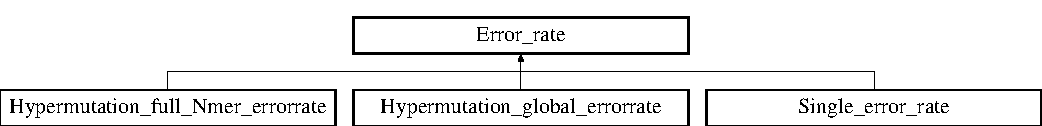
\includegraphics[height=1.696970cm]{dc/d6f/classError__rate}
\end{center}
\end{figure}
\subsection*{Public Member Functions}
\begin{DoxyCompactItemize}
\item 
\mbox{\Hypertarget{classError__rate_a85ce800379f3365e1f1e40d0ad4f27d6}\label{classError__rate_a85ce800379f3365e1f1e40d0ad4f27d6}} 
virtual double {\bfseries compare\+\_\+sequences\+\_\+error\+\_\+prob} (double, const std\+::string \&, \hyperlink{classEnum__fast__memory__map}{Seq\+\_\+type\+\_\+str\+\_\+p\+\_\+map} \&, const \hyperlink{classEnum__fast__memory__dual__key__map}{Seq\+\_\+offsets\+\_\+map} \&, const std\+::unordered\+\_\+map$<$ std\+::tuple$<$ Event\+\_\+type, Gene\+\_\+class, Seq\+\_\+side $>$, std\+::shared\+\_\+ptr$<$ \hyperlink{classRec__Event}{Rec\+\_\+\+Event} $>$$>$ \&, \hyperlink{classEnum__fast__memory__map}{Mismatch\+\_\+vectors\+\_\+map} \&, double \&, double \&)=0
\item 
\mbox{\Hypertarget{classError__rate_abda427d21d09f851fc6a497abf0e0d41}\label{classError__rate_abda427d21d09f851fc6a497abf0e0d41}} 
virtual void {\bfseries update} ()=0
\item 
\mbox{\Hypertarget{classError__rate_a1fbed484799dacb10510628f2a107e7e}\label{classError__rate_a1fbed484799dacb10510628f2a107e7e}} 
virtual void {\bfseries initialize} (const std\+::unordered\+\_\+map$<$ std\+::tuple$<$ Event\+\_\+type, Gene\+\_\+class, Seq\+\_\+side $>$, std\+::shared\+\_\+ptr$<$ \hyperlink{classRec__Event}{Rec\+\_\+\+Event} $>$$>$ \&)
\item 
\mbox{\Hypertarget{classError__rate_a59c2011cf8eb4a79ab9d4560c1cdc3c6}\label{classError__rate_a59c2011cf8eb4a79ab9d4560c1cdc3c6}} 
bool {\bfseries is\+\_\+updated} () const
\item 
\mbox{\Hypertarget{classError__rate_ac4aa825ecaa851b880c2e6094c1eb0fd}\label{classError__rate_ac4aa825ecaa851b880c2e6094c1eb0fd}} 
void {\bfseries update\+\_\+value} (bool update\+\_\+status)
\item 
\mbox{\Hypertarget{classError__rate_a565ac6d0924f7fe4321cd0a0ef802825}\label{classError__rate_a565ac6d0924f7fe4321cd0a0ef802825}} 
virtual void {\bfseries add\+\_\+to\+\_\+norm\+\_\+counter} ()=0
\item 
\mbox{\Hypertarget{classError__rate_ae481534229fc21de79b66d8edcc17d62}\label{classError__rate_ae481534229fc21de79b66d8edcc17d62}} 
virtual void {\bfseries clean\+\_\+seq\+\_\+counters} ()=0
\item 
\mbox{\Hypertarget{classError__rate_ae93054df4880e8fd59770e6a091768c9}\label{classError__rate_ae93054df4880e8fd59770e6a091768c9}} 
void {\bfseries norm\+\_\+weights\+\_\+by\+\_\+seq\+\_\+likelihood} (Marginal\+\_\+array\+\_\+p \&, const size\+\_\+t, const double seq\+\_\+weight=1)
\item 
\mbox{\Hypertarget{classError__rate_a03773cbdcb52e0a231ee42f5bdce5cdc}\label{classError__rate_a03773cbdcb52e0a231ee42f5bdce5cdc}} 
virtual void {\bfseries write2txt} (std\+::ofstream \&)=0
\item 
\mbox{\Hypertarget{classError__rate_a86eff4f0308e3232de4fd54bbdc93c04}\label{classError__rate_a86eff4f0308e3232de4fd54bbdc93c04}} 
virtual std\+::shared\+\_\+ptr$<$ \hyperlink{classError__rate}{Error\+\_\+rate} $>$ {\bfseries copy} () const =0
\item 
\mbox{\Hypertarget{classError__rate_ad170cdf5e6c4825f4ca3bf7a8d7b254f}\label{classError__rate_ad170cdf5e6c4825f4ca3bf7a8d7b254f}} 
virtual std\+::string {\bfseries type} () const =0
\item 
\mbox{\Hypertarget{classError__rate_a5d5a7bde961ef0bd9ae5e22156b18552}\label{classError__rate_a5d5a7bde961ef0bd9ae5e22156b18552}} 
virtual \hyperlink{classError__rate}{Error\+\_\+rate} $\ast$ {\bfseries add\+\_\+checked} (\hyperlink{classError__rate}{Error\+\_\+rate} $\ast$)=0
\item 
\mbox{\Hypertarget{classError__rate_aa2dd5f87d6550df93542d598f546df44}\label{classError__rate_aa2dd5f87d6550df93542d598f546df44}} 
double {\bfseries get\+\_\+model\+\_\+likelihood} () const
\item 
\mbox{\Hypertarget{classError__rate_a4d7037b07adf8cca2d0a173f867749e0}\label{classError__rate_a4d7037b07adf8cca2d0a173f867749e0}} 
double {\bfseries get\+\_\+seq\+\_\+likelihood} () const
\item 
\mbox{\Hypertarget{classError__rate_a41990ead366e9882289ddedb6bfd64be}\label{classError__rate_a41990ead366e9882289ddedb6bfd64be}} 
double {\bfseries get\+\_\+seq\+\_\+probability} () const
\item 
\mbox{\Hypertarget{classError__rate_a28d3b3140dec1002e4ae05f0c4bcc4cd}\label{classError__rate_a28d3b3140dec1002e4ae05f0c4bcc4cd}} 
double {\bfseries get\+\_\+seq\+\_\+mean\+\_\+error\+\_\+number} () const
\item 
\mbox{\Hypertarget{classError__rate_ac66afd48ecfe612c9c0d2751372de620}\label{classError__rate_ac66afd48ecfe612c9c0d2751372de620}} 
virtual const double \& {\bfseries get\+\_\+err\+\_\+rate\+\_\+upper\+\_\+bound} (size\+\_\+t, size\+\_\+t)=0
\item 
\mbox{\Hypertarget{classError__rate_a5ee5de524e97762d18b33d48f5bb82ad}\label{classError__rate_a5ee5de524e97762d18b33d48f5bb82ad}} 
virtual void {\bfseries build\+\_\+upper\+\_\+bound\+\_\+matrix} (size\+\_\+t, size\+\_\+t)=0
\item 
\mbox{\Hypertarget{classError__rate_a8f8fb2d0d60985a660070e5b523d4139}\label{classError__rate_a8f8fb2d0d60985a660070e5b523d4139}} 
virtual int {\bfseries get\+\_\+number\+\_\+non\+\_\+zero\+\_\+likelihood\+\_\+seqs} () const =0
\item 
\mbox{\Hypertarget{classError__rate_acb786947d2b19bee160e49e37d87f2f6}\label{classError__rate_acb786947d2b19bee160e49e37d87f2f6}} 
virtual std\+::queue$<$ int $>$ {\bfseries generate\+\_\+errors} (std\+::string \&, std\+::mt19937\+\_\+64 \&) const =0
\item 
\mbox{\Hypertarget{classError__rate_aaf23376c6c60b95f7b4a798dd0b28691}\label{classError__rate_aaf23376c6c60b95f7b4a798dd0b28691}} 
void {\bfseries set\+\_\+viterbi\+\_\+run} (bool viterbi\+\_\+like)
\end{DoxyCompactItemize}
\subsection*{Public Attributes}
\begin{DoxyCompactItemize}
\item 
\mbox{\Hypertarget{classError__rate_a332b99f1f3ff28228f552297cbbb471e}\label{classError__rate_a332b99f1f3ff28228f552297cbbb471e}} 
int {\bfseries debug\+\_\+number\+\_\+scenarios}
\end{DoxyCompactItemize}
\subsection*{Protected Attributes}
\begin{DoxyCompactItemize}
\item 
\mbox{\Hypertarget{classError__rate_ad65514e6bef52d765159276d8c2e4555}\label{classError__rate_ad65514e6bef52d765159276d8c2e4555}} 
bool {\bfseries updated}
\item 
\mbox{\Hypertarget{classError__rate_a88fbd252630f486e1eb9ae76c8d97205}\label{classError__rate_a88fbd252630f486e1eb9ae76c8d97205}} 
long double {\bfseries model\+\_\+log\+\_\+likelihood}
\item 
\mbox{\Hypertarget{classError__rate_a8ab2a2ff3e951d38f7775bcbad794c53}\label{classError__rate_a8ab2a2ff3e951d38f7775bcbad794c53}} 
int {\bfseries number\+\_\+seq}
\item 
\mbox{\Hypertarget{classError__rate_acb4948fe7aedc104a1e36a21a544f7c2}\label{classError__rate_acb4948fe7aedc104a1e36a21a544f7c2}} 
long double {\bfseries seq\+\_\+likelihood}
\item 
\mbox{\Hypertarget{classError__rate_aeb1808d4631732d10ad921075da48a2a}\label{classError__rate_aeb1808d4631732d10ad921075da48a2a}} 
double {\bfseries seq\+\_\+mean\+\_\+error\+\_\+number}
\item 
\mbox{\Hypertarget{classError__rate_a66750e4559780ed2c0f38f30761494c5}\label{classError__rate_a66750e4559780ed2c0f38f30761494c5}} 
long double {\bfseries scenario\+\_\+new\+\_\+proba}
\item 
\mbox{\Hypertarget{classError__rate_ad5c94788f8932da10e863b677644277e}\label{classError__rate_ad5c94788f8932da10e863b677644277e}} 
long double {\bfseries seq\+\_\+probability}
\item 
\mbox{\Hypertarget{classError__rate_a37803a110ad032624ad5b528290a6d01}\label{classError__rate_a37803a110ad032624ad5b528290a6d01}} 
bool {\bfseries viterbi\+\_\+run}
\item 
\mbox{\Hypertarget{classError__rate_a4690df19a431a3b3de07173117ad9cba}\label{classError__rate_a4690df19a431a3b3de07173117ad9cba}} 
\hyperlink{structMatrix}{Matrix}$<$ double $>$ {\bfseries upper\+\_\+bound\+\_\+proba\+\_\+mat}
\item 
\mbox{\Hypertarget{classError__rate_a8081ac69bdf77964721cccf034bb8752}\label{classError__rate_a8081ac69bdf77964721cccf034bb8752}} 
size\+\_\+t {\bfseries max\+\_\+err}
\item 
\mbox{\Hypertarget{classError__rate_adcf9e8c4fa714b05bf025ccd0bada2a5}\label{classError__rate_adcf9e8c4fa714b05bf025ccd0bada2a5}} 
size\+\_\+t {\bfseries max\+\_\+noerr}
\end{DoxyCompactItemize}


\subsection{Detailed Description}
Abstract class for generic error models behavior. 

\begin{DoxyAuthor}{Author}
Q.\+Marcou 
\end{DoxyAuthor}
\begin{DoxyVersion}{Version}
1.\+0
\end{DoxyVersion}
Base class for defining different error models such as additive or non-\/additive hypermutation models. Errors are assessed when all Rec\+Event iterate have been processed (terminal leaf of the scenario tree) 

The documentation for this class was generated from the following files\+:\begin{DoxyCompactItemize}
\item 
Errorrate.\+h\item 
Errorrate.\+cpp\end{DoxyCompactItemize}

\hypertarget{classErrors__counter}{}\section{Errors\+\_\+counter Class Reference}
\label{classErrors__counter}\index{Errors\+\_\+counter@{Errors\+\_\+counter}}


\hyperlink{classCounter}{Counter} recording the number of genomic nucleotides and errors/mismatch per scenario.  




{\ttfamily \#include $<$Errorscounter.\+h$>$}

Inheritance diagram for Errors\+\_\+counter\+:\begin{figure}[H]
\begin{center}
\leavevmode
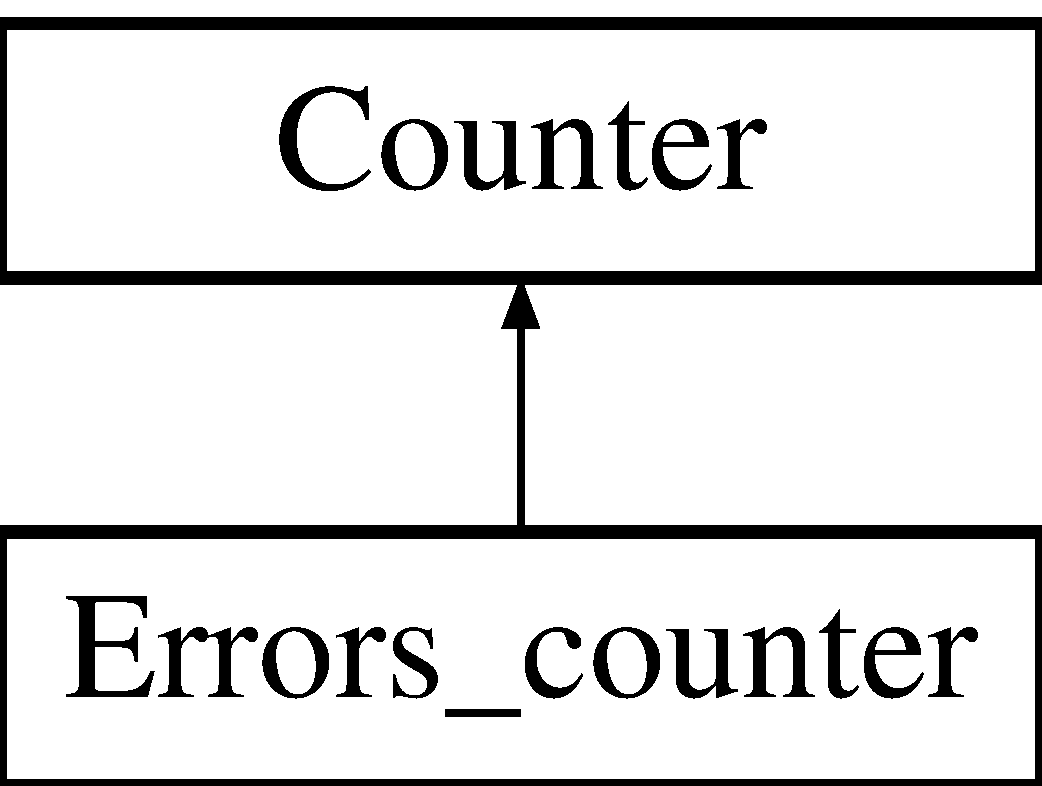
\includegraphics[height=2.000000cm]{d5/d0d/classErrors__counter}
\end{center}
\end{figure}
\subsection*{Public Member Functions}
\begin{DoxyCompactItemize}
\item 
\mbox{\Hypertarget{classErrors__counter_af81869dca1c7eb7f48eef6dc8136517b}\label{classErrors__counter_af81869dca1c7eb7f48eef6dc8136517b}} 
{\bfseries Errors\+\_\+counter} (size\+\_\+t)
\item 
\mbox{\Hypertarget{classErrors__counter_ab493a9d65b00847775341f7e30419488}\label{classErrors__counter_ab493a9d65b00847775341f7e30419488}} 
{\bfseries Errors\+\_\+counter} (size\+\_\+t, bool)
\item 
\mbox{\Hypertarget{classErrors__counter_aae46dd0bba1958343e486750d2e973a9}\label{classErrors__counter_aae46dd0bba1958343e486750d2e973a9}} 
{\bfseries Errors\+\_\+counter} (size\+\_\+t, std\+::string)
\item 
\mbox{\Hypertarget{classErrors__counter_a8f570677df85809d45610899941b6f01}\label{classErrors__counter_a8f570677df85809d45610899941b6f01}} 
{\bfseries Errors\+\_\+counter} (size\+\_\+t, std\+::string, bool)
\item 
\mbox{\Hypertarget{classErrors__counter_a76c7bd69579763b36b3f110fcfcc53c2}\label{classErrors__counter_a76c7bd69579763b36b3f110fcfcc53c2}} 
std\+::string {\bfseries type} () const
\item 
\mbox{\Hypertarget{classErrors__counter_afebd470d99db9d51f737b30f12395052}\label{classErrors__counter_afebd470d99db9d51f737b30f12395052}} 
void {\bfseries initialize\+\_\+counter} (const \hyperlink{classModel__Parms}{Model\+\_\+\+Parms} \&, const \hyperlink{classModel__marginals}{Model\+\_\+marginals} \&)
\item 
\mbox{\Hypertarget{classErrors__counter_aa1a3ac389f93b7498b92ec72d1eb9538}\label{classErrors__counter_aa1a3ac389f93b7498b92ec72d1eb9538}} 
void {\bfseries count\+\_\+scenario} (long double, double, const std\+::string \&, \hyperlink{classEnum__fast__memory__map}{Seq\+\_\+type\+\_\+str\+\_\+p\+\_\+map} \&, const \hyperlink{classEnum__fast__memory__dual__key__map}{Seq\+\_\+offsets\+\_\+map} \&, const std\+::unordered\+\_\+map$<$ std\+::tuple$<$ Event\+\_\+type, Gene\+\_\+class, Seq\+\_\+side $>$, std\+::shared\+\_\+ptr$<$ \hyperlink{classRec__Event}{Rec\+\_\+\+Event} $>$$>$ \&, \hyperlink{classEnum__fast__memory__map}{Mismatch\+\_\+vectors\+\_\+map} \&)
\item 
\mbox{\Hypertarget{classErrors__counter_a2ef5445a5ad019983d47639b11a72f4f}\label{classErrors__counter_a2ef5445a5ad019983d47639b11a72f4f}} 
void {\bfseries count\+\_\+sequence} (double, const \hyperlink{classModel__marginals}{Model\+\_\+marginals} \&, const \hyperlink{classModel__Parms}{Model\+\_\+\+Parms} \&)
\item 
\mbox{\Hypertarget{classErrors__counter_a191f0d8497fb67b0eee281e1d7f84785}\label{classErrors__counter_a191f0d8497fb67b0eee281e1d7f84785}} 
void {\bfseries add\+\_\+checked} (std\+::shared\+\_\+ptr$<$ \hyperlink{classCounter}{Counter} $>$)
\item 
\mbox{\Hypertarget{classErrors__counter_ac1b3ce556c526d2d37d2a3f9b7aba70f}\label{classErrors__counter_ac1b3ce556c526d2d37d2a3f9b7aba70f}} 
void {\bfseries dump\+\_\+sequence\+\_\+data} (int, int)
\item 
\mbox{\Hypertarget{classErrors__counter_aef05dba628412777900fe1f617378d6f}\label{classErrors__counter_aef05dba628412777900fe1f617378d6f}} 
std\+::shared\+\_\+ptr$<$ \hyperlink{classCounter}{Counter} $>$ {\bfseries copy} () const
\end{DoxyCompactItemize}
\subsection*{Additional Inherited Members}


\subsection{Detailed Description}
\hyperlink{classCounter}{Counter} recording the number of genomic nucleotides and errors/mismatch per scenario. 

\begin{DoxyAuthor}{Author}
Q.\+Marcou 
\end{DoxyAuthor}
\begin{DoxyVersion}{Version}
1.\+0
\end{DoxyVersion}
\hyperlink{classCounter}{Counter} recording the number of genomic nucleotides and errors/mismatch per scenario. This information can either be recorded for the N best scenarios or be aggregated to extract individual sequence posterior error/mutation load. 

The documentation for this class was generated from the following files\+:\begin{DoxyCompactItemize}
\item 
Errorscounter.\+h\item 
Errorscounter.\+cpp\end{DoxyCompactItemize}

\hypertarget{structEvent__comparator}{}\section{Event\+\_\+comparator Struct Reference}
\label{structEvent__comparator}\index{Event\+\_\+comparator@{Event\+\_\+comparator}}
\subsection*{Public Member Functions}
\begin{DoxyCompactItemize}
\item 
\mbox{\Hypertarget{structEvent__comparator_a0dbf57478071548eda1b94b36971186b}\label{structEvent__comparator_a0dbf57478071548eda1b94b36971186b}} 
bool {\bfseries operator()} (std\+::shared\+\_\+ptr$<$ const \hyperlink{classRec__Event}{Rec\+\_\+\+Event} $>$ event\+\_\+p1, std\+::shared\+\_\+ptr$<$ const \hyperlink{classRec__Event}{Rec\+\_\+\+Event} $>$ event\+\_\+p2)
\end{DoxyCompactItemize}


The documentation for this struct was generated from the following file\+:\begin{DoxyCompactItemize}
\item 
Rec\+\_\+\+Event.\+h\end{DoxyCompactItemize}

\hypertarget{structEvent__realization}{}\section{Event\+\_\+realization Struct Reference}
\label{structEvent__realization}\index{Event\+\_\+realization@{Event\+\_\+realization}}


Unit that stores an event realization name, value and index.  




{\ttfamily \#include $<$Rec\+\_\+\+Event.\+h$>$}

\subsection*{Public Member Functions}
\begin{DoxyCompactItemize}
\item 
\mbox{\Hypertarget{structEvent__realization_a9556f59a2fbb2969f5a3a47a4efaa7ce}\label{structEvent__realization_a9556f59a2fbb2969f5a3a47a4efaa7ce}} 
{\bfseries Event\+\_\+realization} (std\+::string real\+\_\+name, int val\+\_\+int, std\+::string val\+\_\+str, \hyperlink{classInt__Str}{Int\+\_\+\+Str} val\+\_\+str\+\_\+int, int index\+\_\+val)
\end{DoxyCompactItemize}
\subsection*{Public Attributes}
\begin{DoxyCompactItemize}
\item 
\mbox{\Hypertarget{structEvent__realization_a54404700e07462fe27aa6a7a6faefab9}\label{structEvent__realization_a54404700e07462fe27aa6a7a6faefab9}} 
const std\+::string {\bfseries name}
\item 
\mbox{\Hypertarget{structEvent__realization_a4d4c28a3c4e3caabce32d965a289181e}\label{structEvent__realization_a4d4c28a3c4e3caabce32d965a289181e}} 
const int {\bfseries value\+\_\+int}
\item 
\mbox{\Hypertarget{structEvent__realization_a8ada58ba6fbd31d9c9c3b446581bd13f}\label{structEvent__realization_a8ada58ba6fbd31d9c9c3b446581bd13f}} 
const std\+::string {\bfseries value\+\_\+str}
\item 
\mbox{\Hypertarget{structEvent__realization_af6ed01e953ba786146c6ffb80f03919a}\label{structEvent__realization_af6ed01e953ba786146c6ffb80f03919a}} 
const \hyperlink{classInt__Str}{Int\+\_\+\+Str} {\bfseries value\+\_\+str\+\_\+int}
\item 
\mbox{\Hypertarget{structEvent__realization_aec4a3e1276c59e2585afa7313bc77202}\label{structEvent__realization_aec4a3e1276c59e2585afa7313bc77202}} 
int {\bfseries index}
\end{DoxyCompactItemize}


\subsection{Detailed Description}
Unit that stores an event realization name, value and index. 

\begin{DoxyAuthor}{Author}
Q.\+Marcou 
\end{DoxyAuthor}
\begin{DoxyVersion}{Version}
1.\+0
\end{DoxyVersion}
Depending on the Rec\+Event type to which it belongs, the \hyperlink{structEvent__realization}{Event\+\_\+realization} must supply either a string (both std\+::string and Int\+Str) or an integer value. Integers values are e.\+g the number of deletions or insertions of \hyperlink{classInsertion}{Insertion} or \hyperlink{classDeletion}{Deletion} Rec\+Event String values are e.\+g realization of a Gene\+Choice \hyperlink{classRec__Event}{Rec\+\_\+\+Event}, and stands for the gene sequence. 

The documentation for this struct was generated from the following file\+:\begin{DoxyCompactItemize}
\item 
Rec\+\_\+\+Event.\+h\end{DoxyCompactItemize}

\hypertarget{classExtractFeatures}{}\section{Extract\+Features Class Reference}
\label{classExtractFeatures}\index{Extract\+Features@{Extract\+Features}}


Class to extract sequences features (e.\+g. C\+D\+R3) of sequences using alignment and V, J anchors information.  




{\ttfamily \#include $<$Extract\+Features.\+h$>$}

\subsection*{Public Member Functions}
\begin{DoxyCompactItemize}
\item 
\mbox{\Hypertarget{classExtractFeatures_a7b288f4e64f388d34f1e0cd63cd2dcf6}\label{classExtractFeatures_a7b288f4e64f388d34f1e0cd63cd2dcf6}} 
{\bfseries Extract\+Features} (const \hyperlink{classExtractFeatures}{Extract\+Features} \&orig)
\item 
void \hyperlink{classExtractFeatures_a70b5cef5ad48234649b114dea3eba942}{load\+\_\+\+V\+Jgenomic\+Templates} (vector$<$ pair$<$ string, string $>$$>$ v\+\_\+genomic, vector$<$ pair$<$ string, string $>$$>$ j\+\_\+genomic)
\begin{DoxyCompactList}\small\item\em Function to map the template\+ID and the sequence for V and J. \end{DoxyCompactList}\item 
void \hyperlink{classExtractFeatures_a05f401f4f39adb7f33c2b1e3f7f51807}{load\+\_\+\+V\+Janchors} (string fln\+V\+\_\+\+C\+D\+R3\+\_\+anchors, string fln\+J\+\_\+\+C\+D\+R3\+\_\+anchors)
\begin{DoxyCompactList}\small\item\em load data files into Gene\+Features functor class \end{DoxyCompactList}\item 
void \hyperlink{classExtractFeatures_ace6992bcea2ed1008b5a103291f039c4}{load\+\_\+\+V\+Janchors} (unordered\+\_\+map$<$ string, size\+\_\+t $>$ fln\+V\+\_\+\+C\+D\+R3\+\_\+anchors, unordered\+\_\+map$<$ string, size\+\_\+t $>$ fln\+J\+\_\+\+C\+D\+R3\+\_\+anchors)
\begin{DoxyCompactList}\small\item\em load data files into Gene\+Features functor class \end{DoxyCompactList}\item 
\mbox{\Hypertarget{classExtractFeatures_ac04edfcc22b8b13bdfe24f8786f26df5}\label{classExtractFeatures_ac04edfcc22b8b13bdfe24f8786f26df5}} 
void {\bfseries print\+\_\+\+Vgenomic\+Templates} ()
\item 
\mbox{\Hypertarget{classExtractFeatures_a29cb642660337a3fbaa0446d835ef1fa}\label{classExtractFeatures_a29cb642660337a3fbaa0446d835ef1fa}} 
void {\bfseries print\+\_\+\+Jgenomic\+Templates} ()
\item 
\mbox{\Hypertarget{classExtractFeatures_a79fcd50fc536ec897d7bae410afa1284}\label{classExtractFeatures_a79fcd50fc536ec897d7bae410afa1284}} 
void {\bfseries set\+\_\+sorted\+\_\+alignments} (unordered\+\_\+map$<$ int, pair$<$ string, unordered\+\_\+map$<$ Gene\+\_\+class, vector$<$ \hyperlink{structAlignment__data}{Alignment\+\_\+data} $>$$>$$>$$>$ $\ast$pointer)
\item 
\hyperlink{classCDR3SeqData}{C\+D\+R3\+Seq\+Data} \hyperlink{classExtractFeatures_af1dc5d4f1cb7e15227fbafcd2df662d2}{extract\+C\+D\+R3} (int seq\+\_\+index)
\begin{DoxyCompactList}\small\item\em Get the C\+D\+R3 as an instance of \hyperlink{classCDR3SeqData}{C\+D\+R3\+Seq\+Data} given the V and J \hyperlink{structAlignment__data}{Alignment\+\_\+data} structs. \end{DoxyCompactList}\item 
int \hyperlink{classExtractFeatures_a5d1a024949397722223c20d3fc5e6fd4}{get\+V\+Anchor4\+Seq} (string seq\+\_\+str, \hyperlink{structAlignment__data}{Alignment\+\_\+data} v\+\_\+alig)
\item 
int \hyperlink{classExtractFeatures_a5738a890c09d3cb72ea01693f624b593}{get\+J\+Anchor4\+Seq} (string seq\+\_\+str, \hyperlink{structAlignment__data}{Alignment\+\_\+data} j\+\_\+alig)
\item 
string \hyperlink{classExtractFeatures_aa117a4841d8db720b13c0e0b9028579d}{generate\+C\+D\+R3\+\_\+csv\+\_\+line} (\hyperlink{classCDR3SeqData}{C\+D\+R3\+Seq\+Data} cdr3\+Input\+Seq)
\begin{DoxyCompactList}\small\item\em Function to generate a C\+D\+R3 string line to be printed on a file. \end{DoxyCompactList}\end{DoxyCompactItemize}
\subsection*{Public Attributes}
\begin{DoxyCompactItemize}
\item 
\mbox{\Hypertarget{classExtractFeatures_aa67318cf2f9b155b533a4ab816fdd8ee}\label{classExtractFeatures_aa67318cf2f9b155b533a4ab816fdd8ee}} 
unordered\+\_\+map$<$ string, string $>$ {\bfseries U\+Map\+\_\+v\+\_\+genomic}
\item 
\mbox{\Hypertarget{classExtractFeatures_adf3a835b87f9f274a9b29f830fb7c406}\label{classExtractFeatures_adf3a835b87f9f274a9b29f830fb7c406}} 
unordered\+\_\+map$<$ string, string $>$ {\bfseries U\+Map\+\_\+j\+\_\+genomic}
\item 
\mbox{\Hypertarget{classExtractFeatures_a11a5252b3e1bd2c12b816dbf3f1cff37}\label{classExtractFeatures_a11a5252b3e1bd2c12b816dbf3f1cff37}} 
unordered\+\_\+map$<$ string, size\+\_\+t $>$ {\bfseries U\+Map\+\_\+v\+\_\+\+C\+D\+R3\+\_\+anchors}
\item 
\mbox{\Hypertarget{classExtractFeatures_af524e782f4053ae78c0d12374b6ae6f3}\label{classExtractFeatures_af524e782f4053ae78c0d12374b6ae6f3}} 
unordered\+\_\+map$<$ string, size\+\_\+t $>$ {\bfseries U\+Map\+\_\+j\+\_\+\+C\+D\+R3\+\_\+anchors}
\item 
\mbox{\Hypertarget{classExtractFeatures_a8f90e1dce7c28bc411cebfd72cd63257}\label{classExtractFeatures_a8f90e1dce7c28bc411cebfd72cd63257}} 
unordered\+\_\+map$<$ int, pair$<$ string, unordered\+\_\+map$<$ Gene\+\_\+class, vector$<$ \hyperlink{structAlignment__data}{Alignment\+\_\+data} $>$ $>$ $>$ $>$ $\ast$ {\bfseries p\+\_\+sorted\+\_\+alignments}
\end{DoxyCompactItemize}


\subsection{Detailed Description}
Class to extract sequences features (e.\+g. C\+D\+R3) of sequences using alignment and V, J anchors information. 

\begin{DoxyAuthor}{Author}
C. Olivares 
\end{DoxyAuthor}


\subsection{Member Function Documentation}
\mbox{\Hypertarget{classExtractFeatures_af1dc5d4f1cb7e15227fbafcd2df662d2}\label{classExtractFeatures_af1dc5d4f1cb7e15227fbafcd2df662d2}} 
\index{Extract\+Features@{Extract\+Features}!extract\+C\+D\+R3@{extract\+C\+D\+R3}}
\index{extract\+C\+D\+R3@{extract\+C\+D\+R3}!Extract\+Features@{Extract\+Features}}
\subsubsection{\texorpdfstring{extract\+C\+D\+R3()}{extractCDR3()}}
{\footnotesize\ttfamily \hyperlink{classCDR3SeqData}{C\+D\+R3\+Seq\+Data} Extract\+Features\+::extract\+C\+D\+R3 (\begin{DoxyParamCaption}\item[{int}]{seq\+\_\+index }\end{DoxyParamCaption})}



Get the C\+D\+R3 as an instance of \hyperlink{classCDR3SeqData}{C\+D\+R3\+Seq\+Data} given the V and J \hyperlink{structAlignment__data}{Alignment\+\_\+data} structs. 


\begin{DoxyParams}{Parameters}
{\em seq\+\_\+index} & \\
\hline
{\em V\+\_\+alignment} & \\
\hline
{\em J\+\_\+alignment} & \\
\hline
\end{DoxyParams}
\begin{DoxyReturn}{Returns}
\hyperlink{classCDR3SeqData}{C\+D\+R3\+Seq\+Data} 
\end{DoxyReturn}
\mbox{\Hypertarget{classExtractFeatures_aa117a4841d8db720b13c0e0b9028579d}\label{classExtractFeatures_aa117a4841d8db720b13c0e0b9028579d}} 
\index{Extract\+Features@{Extract\+Features}!generate\+C\+D\+R3\+\_\+csv\+\_\+line@{generate\+C\+D\+R3\+\_\+csv\+\_\+line}}
\index{generate\+C\+D\+R3\+\_\+csv\+\_\+line@{generate\+C\+D\+R3\+\_\+csv\+\_\+line}!Extract\+Features@{Extract\+Features}}
\subsubsection{\texorpdfstring{generate\+C\+D\+R3\+\_\+csv\+\_\+line()}{generateCDR3\_csv\_line()}}
{\footnotesize\ttfamily string Extract\+Features\+::generate\+C\+D\+R3\+\_\+csv\+\_\+line (\begin{DoxyParamCaption}\item[{\hyperlink{classCDR3SeqData}{C\+D\+R3\+Seq\+Data}}]{cdr3\+Input\+Seq }\end{DoxyParamCaption})}



Function to generate a C\+D\+R3 string line to be printed on a file. 


\begin{DoxyParams}{Parameters}
{\em cdr3\+Input\+Seq} & is \hyperlink{classCDR3SeqData}{C\+D\+R3\+Seq\+Data} instance \\
\hline
\end{DoxyParams}
\begin{DoxyReturn}{Returns}
csvline line string to be printed on a file. 
\end{DoxyReturn}
\mbox{\Hypertarget{classExtractFeatures_a5738a890c09d3cb72ea01693f624b593}\label{classExtractFeatures_a5738a890c09d3cb72ea01693f624b593}} 
\index{Extract\+Features@{Extract\+Features}!get\+J\+Anchor4\+Seq@{get\+J\+Anchor4\+Seq}}
\index{get\+J\+Anchor4\+Seq@{get\+J\+Anchor4\+Seq}!Extract\+Features@{Extract\+Features}}
\subsubsection{\texorpdfstring{get\+J\+Anchor4\+Seq()}{getJAnchor4Seq()}}
{\footnotesize\ttfamily int Extract\+Features\+::get\+J\+Anchor4\+Seq (\begin{DoxyParamCaption}\item[{string}]{seq\+\_\+str,  }\item[{\hyperlink{structAlignment__data}{Alignment\+\_\+data}}]{j\+\_\+alig }\end{DoxyParamCaption})}

Calculate the J anchor in reference to the input sequence 
\begin{DoxyParams}{Parameters}
{\em seq\+\_\+str} & \\
\hline
{\em j\+\_\+alig} & \\
\hline
\end{DoxyParams}
\begin{DoxyReturn}{Returns}
cdr3\+\_\+j\+\_\+read\+\_\+anch the anchor in reference to the input sequence. 
\end{DoxyReturn}
\mbox{\Hypertarget{classExtractFeatures_a5d1a024949397722223c20d3fc5e6fd4}\label{classExtractFeatures_a5d1a024949397722223c20d3fc5e6fd4}} 
\index{Extract\+Features@{Extract\+Features}!get\+V\+Anchor4\+Seq@{get\+V\+Anchor4\+Seq}}
\index{get\+V\+Anchor4\+Seq@{get\+V\+Anchor4\+Seq}!Extract\+Features@{Extract\+Features}}
\subsubsection{\texorpdfstring{get\+V\+Anchor4\+Seq()}{getVAnchor4Seq()}}
{\footnotesize\ttfamily int Extract\+Features\+::get\+V\+Anchor4\+Seq (\begin{DoxyParamCaption}\item[{string}]{seq\+\_\+str,  }\item[{\hyperlink{structAlignment__data}{Alignment\+\_\+data}}]{v\+\_\+alig }\end{DoxyParamCaption})}

Calculate the V anchor in reference to the input sequence 
\begin{DoxyParams}{Parameters}
{\em seq\+\_\+str} & \\
\hline
{\em v\+\_\+alig} & \\
\hline
\end{DoxyParams}
\begin{DoxyReturn}{Returns}
cdr3\+\_\+v\+\_\+read\+\_\+anch the anchor in reference to the input sequence. 
\end{DoxyReturn}
\mbox{\Hypertarget{classExtractFeatures_a05f401f4f39adb7f33c2b1e3f7f51807}\label{classExtractFeatures_a05f401f4f39adb7f33c2b1e3f7f51807}} 
\index{Extract\+Features@{Extract\+Features}!load\+\_\+\+V\+Janchors@{load\+\_\+\+V\+Janchors}}
\index{load\+\_\+\+V\+Janchors@{load\+\_\+\+V\+Janchors}!Extract\+Features@{Extract\+Features}}
\subsubsection{\texorpdfstring{load\+\_\+\+V\+Janchors()}{load\_VJanchors()}\hspace{0.1cm}{\footnotesize\ttfamily [1/2]}}
{\footnotesize\ttfamily void Extract\+Features\+::load\+\_\+\+V\+Janchors (\begin{DoxyParamCaption}\item[{string}]{fln\+V\+\_\+\+C\+D\+R3\+\_\+anchors,  }\item[{string}]{fln\+J\+\_\+\+C\+D\+R3\+\_\+anchors }\end{DoxyParamCaption})}



load data files into Gene\+Features functor class 


\begin{DoxyParams}{Parameters}
{\em fln\+V\+\_\+\+C\+D\+R3\+\_\+anchors} & C\+D\+R3 anchors filename for V genes \\
\hline
{\em fln\+J\+\_\+\+C\+D\+R3\+\_\+anchors} & C\+D\+R3 anchors filename for J genes \\
\hline
\end{DoxyParams}
\mbox{\Hypertarget{classExtractFeatures_ace6992bcea2ed1008b5a103291f039c4}\label{classExtractFeatures_ace6992bcea2ed1008b5a103291f039c4}} 
\index{Extract\+Features@{Extract\+Features}!load\+\_\+\+V\+Janchors@{load\+\_\+\+V\+Janchors}}
\index{load\+\_\+\+V\+Janchors@{load\+\_\+\+V\+Janchors}!Extract\+Features@{Extract\+Features}}
\subsubsection{\texorpdfstring{load\+\_\+\+V\+Janchors()}{load\_VJanchors()}\hspace{0.1cm}{\footnotesize\ttfamily [2/2]}}
{\footnotesize\ttfamily void Extract\+Features\+::load\+\_\+\+V\+Janchors (\begin{DoxyParamCaption}\item[{unordered\+\_\+map$<$ string, size\+\_\+t $>$}]{v\+\_\+\+C\+D\+R3\+\_\+anchors,  }\item[{unordered\+\_\+map$<$ string, size\+\_\+t $>$}]{j\+\_\+\+C\+D\+R3\+\_\+anchors }\end{DoxyParamCaption})}



load data files into Gene\+Features functor class 


\begin{DoxyParams}{Parameters}
{\em v\+\_\+\+C\+D\+R3\+\_\+anchors} & unordered\+\_\+map of sequence description and position for V genes C\+D\+R3 anchors. \\
\hline
{\em j\+\_\+\+C\+D\+R3\+\_\+anchors} & unordered\+\_\+map of sequence description and position for J genes C\+D\+R3 anchors. \\
\hline
\end{DoxyParams}
\mbox{\Hypertarget{classExtractFeatures_a70b5cef5ad48234649b114dea3eba942}\label{classExtractFeatures_a70b5cef5ad48234649b114dea3eba942}} 
\index{Extract\+Features@{Extract\+Features}!load\+\_\+\+V\+Jgenomic\+Templates@{load\+\_\+\+V\+Jgenomic\+Templates}}
\index{load\+\_\+\+V\+Jgenomic\+Templates@{load\+\_\+\+V\+Jgenomic\+Templates}!Extract\+Features@{Extract\+Features}}
\subsubsection{\texorpdfstring{load\+\_\+\+V\+Jgenomic\+Templates()}{load\_VJgenomicTemplates()}}
{\footnotesize\ttfamily void Extract\+Features\+::load\+\_\+\+V\+Jgenomic\+Templates (\begin{DoxyParamCaption}\item[{vector$<$ pair$<$ string, string $>$$>$}]{v\+\_\+genomic,  }\item[{vector$<$ pair$<$ string, string $>$$>$}]{j\+\_\+genomic }\end{DoxyParamCaption})}



Function to map the template\+ID and the sequence for V and J. 


\begin{DoxyParams}{Parameters}
{\em v\+\_\+genomic} & vector with the genomic templates for V genes \\
\hline
{\em j\+\_\+genomic} & vector with the genomic templates for J genes \\
\hline
\end{DoxyParams}
\begin{DoxyReturn}{Returns}

\end{DoxyReturn}


The documentation for this class was generated from the following files\+:\begin{DoxyCompactItemize}
\item 
Extract\+Features.\+h\item 
Extract\+Features.\+cpp\end{DoxyCompactItemize}

\hypertarget{structgen__CDR3__data}{}\section{gen\+\_\+\+C\+D\+R3\+\_\+data Struct Reference}
\label{structgen__CDR3__data}\index{gen\+\_\+\+C\+D\+R3\+\_\+data@{gen\+\_\+\+C\+D\+R3\+\_\+data}}


{\ttfamily \#include $<$Gen\+Model.\+h$>$}

\subsection*{Public Member Functions}
\begin{DoxyCompactItemize}
\item 
\mbox{\Hypertarget{structgen__CDR3__data_a84bc07450f621034cd1f7f2db9cc2270}\label{structgen__CDR3__data_a84bc07450f621034cd1f7f2db9cc2270}} 
{\bfseries gen\+\_\+\+C\+D\+R3\+\_\+data} (const std\+::unordered\+\_\+map$<$ std\+::string, size\+\_\+t $>$ \&v\+\_\+anchors\+\_\+indices, const std\+::unordered\+\_\+map$<$ std\+::string, \hyperlink{structEvent__realization}{Event\+\_\+realization} $>$ \&v\+\_\+reals, size\+\_\+t v\+\_\+event\+\_\+pos, const std\+::unordered\+\_\+map$<$ std\+::string, size\+\_\+t $>$ \&j\+\_\+anchors\+\_\+indices, const std\+::unordered\+\_\+map$<$ std\+::string, \hyperlink{structEvent__realization}{Event\+\_\+realization} $>$ \&j\+\_\+reals, size\+\_\+t j\+\_\+event\+\_\+pos, std\+::shared\+\_\+ptr$<$ std\+::ostream $>$ output\+\_\+stream\+\_\+ptr=std\+::shared\+\_\+ptr$<$ std\+::ostream $>$(\&std\+::cout, \hyperlink{structnull__delete}{null\+\_\+delete}$<$ std\+::ostream $>$()))
\end{DoxyCompactItemize}
\subsection*{Public Attributes}
\begin{DoxyCompactItemize}
\item 
\mbox{\Hypertarget{structgen__CDR3__data_a7f92109048f58a87470b73caacebde6d}\label{structgen__CDR3__data_a7f92109048f58a87470b73caacebde6d}} 
std\+::map$<$ int, std\+::tuple$<$ std\+::string, size\+\_\+t, size\+\_\+t, std\+::string $>$ $>$ {\bfseries v\+\_\+anchors}
\item 
\mbox{\Hypertarget{structgen__CDR3__data_ac3afce3cadecec66b19eaa8fe7cd02e0}\label{structgen__CDR3__data_ac3afce3cadecec66b19eaa8fe7cd02e0}} 
size\+\_\+t {\bfseries v\+\_\+event\+\_\+queue\+\_\+position}
\item 
\mbox{\Hypertarget{structgen__CDR3__data_a74593eab758b80924d97f46ec9946157}\label{structgen__CDR3__data_a74593eab758b80924d97f46ec9946157}} 
std\+::map$<$ int, std\+::tuple$<$ std\+::string, size\+\_\+t, size\+\_\+t, std\+::string $>$ $>$ {\bfseries j\+\_\+anchors}
\item 
\mbox{\Hypertarget{structgen__CDR3__data_af902c78f5810850245e5afcb0e9d183e}\label{structgen__CDR3__data_af902c78f5810850245e5afcb0e9d183e}} 
size\+\_\+t {\bfseries j\+\_\+event\+\_\+queue\+\_\+position}
\item 
\mbox{\Hypertarget{structgen__CDR3__data_aaa951daedffb5700881229b510c9b39f}\label{structgen__CDR3__data_aaa951daedffb5700881229b510c9b39f}} 
std\+::shared\+\_\+ptr$<$ std\+::ostream $>$ {\bfseries output\+\_\+stream}
\item 
\mbox{\Hypertarget{structgen__CDR3__data_acde307f0050ad91e75bd9b63a6252c5e}\label{structgen__CDR3__data_acde307f0050ad91e75bd9b63a6252c5e}} 
bool {\bfseries output\+\_\+nt\+\_\+\+C\+D\+R3} = true
\item 
\mbox{\Hypertarget{structgen__CDR3__data_a0fb27bb73315b9c76d20171fa21d2f7e}\label{structgen__CDR3__data_a0fb27bb73315b9c76d20171fa21d2f7e}} 
bool {\bfseries output\+\_\+anchors\+\_\+found} = true
\item 
\mbox{\Hypertarget{structgen__CDR3__data_aa6fb61bcdef0cf0f386cc83bba01e69a}\label{structgen__CDR3__data_aa6fb61bcdef0cf0f386cc83bba01e69a}} 
bool {\bfseries output\+\_\+inframe} = true
\item 
\mbox{\Hypertarget{structgen__CDR3__data_aa42f2dd27ef5f7f7ae14391197f4af1c}\label{structgen__CDR3__data_aa42f2dd27ef5f7f7ae14391197f4af1c}} 
bool {\bfseries output\+\_\+aa\+\_\+\+C\+D\+R3} = false
\item 
\mbox{\Hypertarget{structgen__CDR3__data_a469689d75e4111ac6a9aa5c57a3ee67d}\label{structgen__CDR3__data_a469689d75e4111ac6a9aa5c57a3ee67d}} 
bool {\bfseries output\+\_\+productive} = false
\end{DoxyCompactItemize}


\subsection{Detailed Description}
Hardcode a data structure for the function extracting C\+D\+R3s in generated sequences 

The documentation for this struct was generated from the following file\+:\begin{DoxyCompactItemize}
\item 
Gen\+Model.\+h\end{DoxyCompactItemize}

\hypertarget{classGene__choice}{}\section{Gene\+\_\+choice Class Reference}
\label{classGene__choice}\index{Gene\+\_\+choice@{Gene\+\_\+choice}}


Gene\+Choice recombination event.  




{\ttfamily \#include $<$Genechoice.\+h$>$}

Inheritance diagram for Gene\+\_\+choice\+:\begin{figure}[H]
\begin{center}
\leavevmode
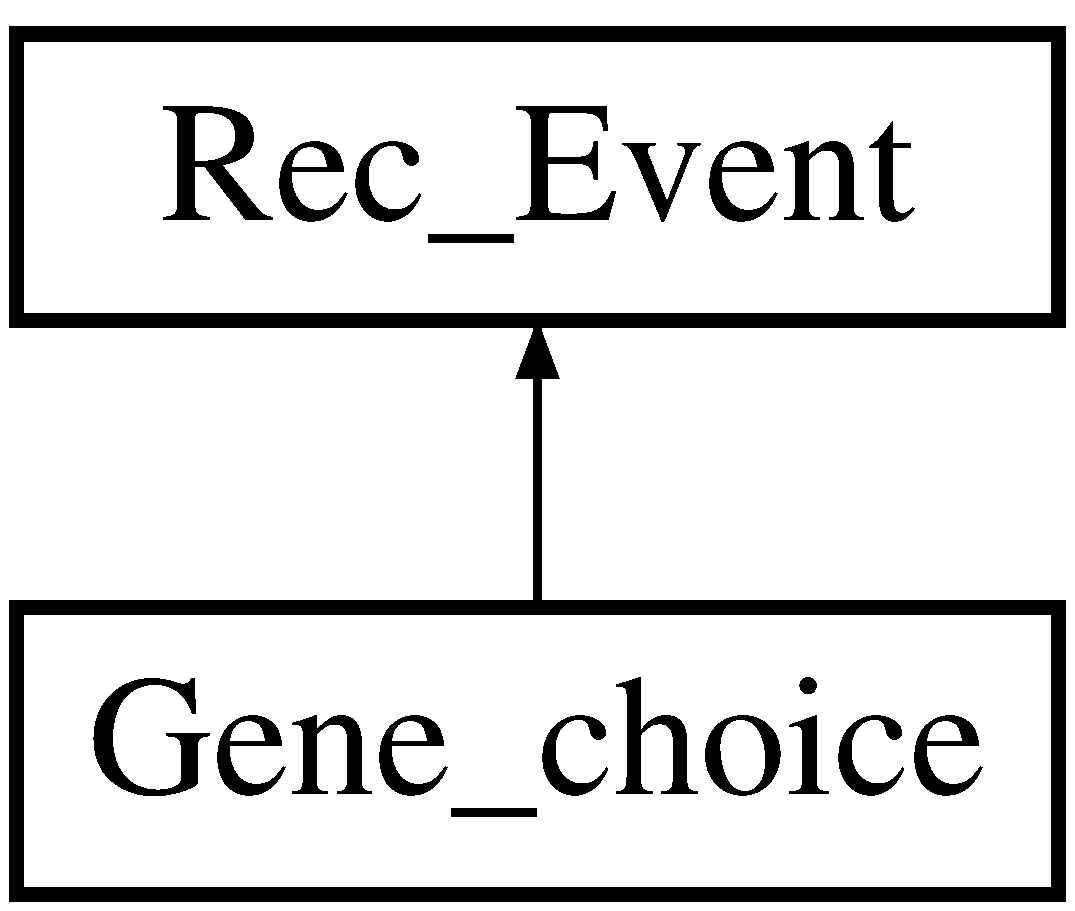
\includegraphics[height=2.000000cm]{df/dae/classGene__choice}
\end{center}
\end{figure}
\subsection*{Public Member Functions}
\begin{DoxyCompactItemize}
\item 
\mbox{\Hypertarget{classGene__choice_aadae79625212bc82c78bce9849e8325a}\label{classGene__choice_aadae79625212bc82c78bce9849e8325a}} 
{\bfseries Gene\+\_\+choice} (Gene\+\_\+class)
\item 
\mbox{\Hypertarget{classGene__choice_a1fcb013e222239211ce0f1137d416157}\label{classGene__choice_a1fcb013e222239211ce0f1137d416157}} 
{\bfseries Gene\+\_\+choice} (Gene\+\_\+class, std\+::unordered\+\_\+map$<$ std\+::string, \hyperlink{structEvent__realization}{Event\+\_\+realization} $>$ \&)
\item 
\mbox{\Hypertarget{classGene__choice_af5558f7c579350c4dc044bd37f26423e}\label{classGene__choice_af5558f7c579350c4dc044bd37f26423e}} 
{\bfseries Gene\+\_\+choice} (Gene\+\_\+class, std\+::vector$<$ std\+::pair$<$ std\+::string, std\+::string $>$$>$)
\item 
\mbox{\Hypertarget{classGene__choice_a04760e99cded10a20cb757de374e2c66}\label{classGene__choice_a04760e99cded10a20cb757de374e2c66}} 
std\+::shared\+\_\+ptr$<$ \hyperlink{classRec__Event}{Rec\+\_\+\+Event} $>$ {\bfseries copy} ()
\item 
void \hyperlink{classGene__choice_ab036f686e32561d4db2aa9eca3be4cf0}{iterate} (double \&, \hyperlink{classEnum__fast__memory__map}{Downstream\+\_\+scenario\+\_\+proba\+\_\+bound\+\_\+map} \&, const std\+::string \&, const \hyperlink{classInt__Str}{Int\+\_\+\+Str} \&, \hyperlink{classEnum__fast__memory__map}{Index\+\_\+map} \&, const std\+::unordered\+\_\+map$<$ Rec\+\_\+\+Event\+\_\+name, std\+::vector$<$ std\+::pair$<$ std\+::shared\+\_\+ptr$<$ const \hyperlink{classRec__Event}{Rec\+\_\+\+Event} $>$, int $>$$>$$>$ \&, std\+::shared\+\_\+ptr$<$ \hyperlink{classRec__Event}{Next\+\_\+event\+\_\+ptr} $>$ \&, Marginal\+\_\+array\+\_\+p \&, const Marginal\+\_\+array\+\_\+p \&, const std\+::unordered\+\_\+map$<$ Gene\+\_\+class, std\+::vector$<$ \hyperlink{structAlignment__data}{Alignment\+\_\+data} $>$$>$ \&, \hyperlink{classEnum__fast__memory__map}{Seq\+\_\+type\+\_\+str\+\_\+p\+\_\+map} \&, \hyperlink{classEnum__fast__memory__dual__key__map}{Seq\+\_\+offsets\+\_\+map} \&, std\+::shared\+\_\+ptr$<$ \hyperlink{classError__rate}{Error\+\_\+rate} $>$ \&, std\+::map$<$ size\+\_\+t, std\+::shared\+\_\+ptr$<$ \hyperlink{classCounter}{Counter} $>$$>$ \&, const std\+::unordered\+\_\+map$<$ std\+::tuple$<$ Event\+\_\+type, Gene\+\_\+class, Seq\+\_\+side $>$, std\+::shared\+\_\+ptr$<$ \hyperlink{classRec__Event}{Rec\+\_\+\+Event} $>$$>$ \&, \hyperlink{classEnum__fast__memory__map}{Safety\+\_\+bool\+\_\+map} \&, \hyperlink{classEnum__fast__memory__map}{Mismatch\+\_\+vectors\+\_\+map} \&, double \&, double \&)
\begin{DoxyCompactList}\small\item\em Evaluate all Event\+\_\+\+Realization of a Rec\+Event for a given sequence. \end{DoxyCompactList}\item 
\mbox{\Hypertarget{classGene__choice_a7b274bb7d2224f66366636cecc487b72}\label{classGene__choice_a7b274bb7d2224f66366636cecc487b72}} 
void {\bfseries add\+\_\+realization} (int)
\item 
\mbox{\Hypertarget{classGene__choice_a77a1eadc4a10c5adfd10b80f3510efbc}\label{classGene__choice_a77a1eadc4a10c5adfd10b80f3510efbc}} 
bool {\bfseries add\+\_\+realization} (std\+::string gene\+\_\+name, std\+::string gene\+\_\+sequence)
\item 
\mbox{\Hypertarget{classGene__choice_a679b1a47747c90b88c7905fbdf5dddc6}\label{classGene__choice_a679b1a47747c90b88c7905fbdf5dddc6}} 
void {\bfseries set\+\_\+genomic\+\_\+templates} (const std\+::vector$<$ std\+::pair$<$ std\+::string, std\+::string $>$$>$ \&)
\item 
\mbox{\Hypertarget{classGene__choice_a5a439725d4a2e1e7b4ebefce7ff5527e}\label{classGene__choice_a5a439725d4a2e1e7b4ebefce7ff5527e}} 
std\+::queue$<$ int $>$ {\bfseries draw\+\_\+random\+\_\+realization} (const Marginal\+\_\+array\+\_\+p \&, std\+::unordered\+\_\+map$<$ Rec\+\_\+\+Event\+\_\+name, int $>$ \&, const std\+::unordered\+\_\+map$<$ Rec\+\_\+\+Event\+\_\+name, std\+::vector$<$ std\+::pair$<$ std\+::shared\+\_\+ptr$<$ const \hyperlink{classRec__Event}{Rec\+\_\+\+Event} $>$, int $>$$>$$>$ \&, std\+::unordered\+\_\+map$<$ Seq\+\_\+type, std\+::string $>$ \&, std\+::mt19937\+\_\+64 \&) const
\item 
\mbox{\Hypertarget{classGene__choice_a9f7c9303d2c0d3a0de6b8098ebf9317b}\label{classGene__choice_a9f7c9303d2c0d3a0de6b8098ebf9317b}} 
void {\bfseries write2txt} (std\+::ofstream \&)
\item 
\mbox{\Hypertarget{classGene__choice_ab76e5a240887c7c8b4b47abe350e52b2}\label{classGene__choice_ab76e5a240887c7c8b4b47abe350e52b2}} 
void {\bfseries initialize\+\_\+event} (std\+::unordered\+\_\+set$<$ Rec\+\_\+\+Event\+\_\+name $>$ \&, const std\+::unordered\+\_\+map$<$ std\+::tuple$<$ Event\+\_\+type, Gene\+\_\+class, Seq\+\_\+side $>$, std\+::shared\+\_\+ptr$<$ \hyperlink{classRec__Event}{Rec\+\_\+\+Event} $>$$>$ \&, const std\+::unordered\+\_\+map$<$ Rec\+\_\+\+Event\+\_\+name, std\+::vector$<$ std\+::pair$<$ std\+::shared\+\_\+ptr$<$ const \hyperlink{classRec__Event}{Rec\+\_\+\+Event} $>$, int $>$$>$$>$ \&, \hyperlink{classEnum__fast__memory__map}{Downstream\+\_\+scenario\+\_\+proba\+\_\+bound\+\_\+map} \&, \hyperlink{classEnum__fast__memory__map}{Seq\+\_\+type\+\_\+str\+\_\+p\+\_\+map} \&, \hyperlink{classEnum__fast__memory__map}{Safety\+\_\+bool\+\_\+map} \&, std\+::shared\+\_\+ptr$<$ \hyperlink{classError__rate}{Error\+\_\+rate} $>$, \hyperlink{classEnum__fast__memory__map}{Mismatch\+\_\+vectors\+\_\+map} \&, \hyperlink{classEnum__fast__memory__dual__key__map}{Seq\+\_\+offsets\+\_\+map} \&, \hyperlink{classEnum__fast__memory__map}{Index\+\_\+map} \&)
\item 
void \hyperlink{classGene__choice_ac1d61da5a319518f24af8da2e1e6435a}{add\+\_\+to\+\_\+marginals} (long double, Marginal\+\_\+array\+\_\+p \&) const
\item 
\mbox{\Hypertarget{classGene__choice_addb3eb932abb73591f123039f06cc4e8}\label{classGene__choice_addb3eb932abb73591f123039f06cc4e8}} 
bool {\bfseries has\+\_\+effect\+\_\+on} (Seq\+\_\+type) const
\item 
\mbox{\Hypertarget{classGene__choice_a6d9d5bb6b3db54ecba7476ad4551f6cc}\label{classGene__choice_a6d9d5bb6b3db54ecba7476ad4551f6cc}} 
void {\bfseries iterate\+\_\+initialize\+\_\+\+Len\+\_\+proba} (Seq\+\_\+type considered\+\_\+junction, std\+::map$<$ int, double $>$ \&length\+\_\+best\+\_\+proba\+\_\+map, std\+::queue$<$ std\+::shared\+\_\+ptr$<$ \hyperlink{classRec__Event}{Rec\+\_\+\+Event} $>$$>$ \&model\+\_\+queue, double \&scenario\+\_\+proba, const Marginal\+\_\+array\+\_\+p \&model\+\_\+parameters\+\_\+point, \hyperlink{classEnum__fast__memory__map}{Index\+\_\+map} \&base\+\_\+index\+\_\+map, \hyperlink{classEnum__fast__memory__map}{Seq\+\_\+type\+\_\+str\+\_\+p\+\_\+map} \&constructed\+\_\+sequences, int \&seq\+\_\+len) const
\item 
\mbox{\Hypertarget{classGene__choice_a916aec7655d44275ffce9f19acee4b4d}\label{classGene__choice_a916aec7655d44275ffce9f19acee4b4d}} 
void {\bfseries initialize\+\_\+\+Len\+\_\+proba\+\_\+bound} (std\+::queue$<$ std\+::shared\+\_\+ptr$<$ \hyperlink{classRec__Event}{Rec\+\_\+\+Event} $>$$>$ \&model\+\_\+queue, const Marginal\+\_\+array\+\_\+p \&model\+\_\+parameters\+\_\+point, \hyperlink{classEnum__fast__memory__map}{Index\+\_\+map} \&base\+\_\+index\+\_\+map)
\end{DoxyCompactItemize}
\subsection*{Friends}
\begin{DoxyCompactItemize}
\item 
\mbox{\Hypertarget{classGene__choice_ad4a26da5a0e142c5135c983af6d042d6}\label{classGene__choice_ad4a26da5a0e142c5135c983af6d042d6}} 
class {\bfseries Coverage\+\_\+err\+\_\+counter}
\item 
\mbox{\Hypertarget{classGene__choice_ad5a47907bf54eec60bc584c426aaca7f}\label{classGene__choice_ad5a47907bf54eec60bc584c426aaca7f}} 
class {\bfseries Hypermutation\+\_\+global\+\_\+errorrate}
\item 
\mbox{\Hypertarget{classGene__choice_a5ff5d89d255ca8ca355c6da8c4be7f68}\label{classGene__choice_a5ff5d89d255ca8ca355c6da8c4be7f68}} 
class {\bfseries Hypermutation\+\_\+full\+\_\+\+Nmer\+\_\+errorrate}
\end{DoxyCompactItemize}
\subsection*{Additional Inherited Members}


\subsection{Detailed Description}
Gene\+Choice recombination event. 

\begin{DoxyAuthor}{Author}
Q.\+Marcou 
\end{DoxyAuthor}
\begin{DoxyVersion}{Version}
1.\+0
\end{DoxyVersion}
Models the gene choice recombination process. The event realizations are explored based on the sequence alignments that were provdided to the inference. Since D gene can be heavily deleted and might not be recognizable by sequence alignments, a special handling of the D gene choice exploring all D positions ranked by their likelihood has been implemented. 

\subsection{Member Function Documentation}
\mbox{\Hypertarget{classGene__choice_ac1d61da5a319518f24af8da2e1e6435a}\label{classGene__choice_ac1d61da5a319518f24af8da2e1e6435a}} 
\index{Gene\+\_\+choice@{Gene\+\_\+choice}!add\+\_\+to\+\_\+marginals@{add\+\_\+to\+\_\+marginals}}
\index{add\+\_\+to\+\_\+marginals@{add\+\_\+to\+\_\+marginals}!Gene\+\_\+choice@{Gene\+\_\+choice}}
\subsubsection{\texorpdfstring{add\+\_\+to\+\_\+marginals()}{add\_to\_marginals()}}
{\footnotesize\ttfamily void Gene\+\_\+choice\+::add\+\_\+to\+\_\+marginals (\begin{DoxyParamCaption}\item[{long double}]{scenario\+\_\+proba,  }\item[{Marginal\+\_\+array\+\_\+p \&}]{updated\+\_\+marginals }\end{DoxyParamCaption}) const\hspace{0.3cm}{\ttfamily [virtual]}}

All add\+\_\+to\+\_\+marginals should take into account the possibility to perform viterbi runs(take only the most likely scenario into account) 

Implements \hyperlink{classRec__Event}{Rec\+\_\+\+Event}.

\mbox{\Hypertarget{classGene__choice_ab036f686e32561d4db2aa9eca3be4cf0}\label{classGene__choice_ab036f686e32561d4db2aa9eca3be4cf0}} 
\index{Gene\+\_\+choice@{Gene\+\_\+choice}!iterate@{iterate}}
\index{iterate@{iterate}!Gene\+\_\+choice@{Gene\+\_\+choice}}
\subsubsection{\texorpdfstring{iterate()}{iterate()}}
{\footnotesize\ttfamily void Gene\+\_\+choice\+::iterate (\begin{DoxyParamCaption}\item[{double \&}]{,  }\item[{\hyperlink{classEnum__fast__memory__map}{Downstream\+\_\+scenario\+\_\+proba\+\_\+bound\+\_\+map} \&}]{,  }\item[{const std\+::string \&}]{,  }\item[{const \hyperlink{classInt__Str}{Int\+\_\+\+Str} \&}]{,  }\item[{\hyperlink{classEnum__fast__memory__map}{Index\+\_\+map} \&}]{,  }\item[{const std\+::unordered\+\_\+map$<$ Rec\+\_\+\+Event\+\_\+name, std\+::vector$<$ std\+::pair$<$ std\+::shared\+\_\+ptr$<$ const \hyperlink{classRec__Event}{Rec\+\_\+\+Event} $>$, int $>$$>$$>$ \&}]{,  }\item[{std\+::shared\+\_\+ptr$<$ \hyperlink{classRec__Event}{Next\+\_\+event\+\_\+ptr} $>$ \&}]{,  }\item[{Marginal\+\_\+array\+\_\+p \&}]{,  }\item[{const Marginal\+\_\+array\+\_\+p \&}]{,  }\item[{const std\+::unordered\+\_\+map$<$ Gene\+\_\+class, std\+::vector$<$ \hyperlink{structAlignment__data}{Alignment\+\_\+data} $>$$>$ \&}]{,  }\item[{\hyperlink{classEnum__fast__memory__map}{Seq\+\_\+type\+\_\+str\+\_\+p\+\_\+map} \&}]{,  }\item[{\hyperlink{classEnum__fast__memory__dual__key__map}{Seq\+\_\+offsets\+\_\+map} \&}]{,  }\item[{std\+::shared\+\_\+ptr$<$ \hyperlink{classError__rate}{Error\+\_\+rate} $>$ \&}]{,  }\item[{std\+::map$<$ size\+\_\+t, std\+::shared\+\_\+ptr$<$ \hyperlink{classCounter}{Counter} $>$$>$ \&}]{,  }\item[{const std\+::unordered\+\_\+map$<$ std\+::tuple$<$ Event\+\_\+type, Gene\+\_\+class, Seq\+\_\+side $>$, std\+::shared\+\_\+ptr$<$ \hyperlink{classRec__Event}{Rec\+\_\+\+Event} $>$$>$ \&}]{,  }\item[{\hyperlink{classEnum__fast__memory__map}{Safety\+\_\+bool\+\_\+map} \&}]{,  }\item[{\hyperlink{classEnum__fast__memory__map}{Mismatch\+\_\+vectors\+\_\+map} \&}]{,  }\item[{double \&}]{,  }\item[{double \&}]{ }\end{DoxyParamCaption})\hspace{0.3cm}{\ttfamily [inline]}, {\ttfamily [virtual]}}



Evaluate all Event\+\_\+\+Realization of a Rec\+Event for a given sequence. 

\begin{DoxyAuthor}{Author}
Q.\+Marcou 
\end{DoxyAuthor}
\begin{DoxyVersion}{Version}
1.\+0 
\end{DoxyVersion}

\begin{DoxyParams}[1]{Parameters}
\mbox{\tt in,out}  & {\em scenario\+\_\+proba} & Probability of the currently explored (incomplete) scenario \\
\hline
\mbox{\tt in,out}  & {\em downstream\+\_\+proba\+\_\+map} & \\
\hline
\mbox{\tt in}  & {\em sequence} & The studied sequence in nucleotide code \\
\hline
\mbox{\tt in}  & {\em int\+\_\+sequence} & The studied sequence in integer code \\
\hline
\mbox{\tt in,out}  & {\em base\+\_\+index\+\_\+map} & Dynamic map recording where probabilities should be read on the marginals. \\
\hline
\mbox{\tt in}  & {\em offset\+\_\+map} & Tells the event by how much indices from the children events should be modified \\
\hline
\mbox{\tt in}  & {\em next\+\_\+event\+\_\+ptr\+\_\+arr} & Indicates the next event to call iterate on \\
\hline
\mbox{\tt in}  & {\em updated\+\_\+marginals\+\_\+point} & Summary marginals on which complete scenario posteriors are recorded \\
\hline
\mbox{\tt in}  & {\em model\+\_\+parameters\+\_\+point} & Current recombination probability distribution \\
\hline
\mbox{\tt in}  & {\em allowed\+\_\+realizations} & The set of genomic templates alignment \\
\hline
\mbox{\tt in,out}  & {\em constructed\+\_\+sequences} & Map containing the (incomplete) scenario\textquotesingle{}s resulting sequence \\
\hline
\mbox{\tt in,out}  & {\em seq\+\_\+offsets} & Map containing the 3\textquotesingle{} and 5\textquotesingle{} offsets of each scenario sequence piece \\
\hline
\mbox{\tt in}  & {\em error\+\_\+rate\+\_\+p} & Pointer to the error model object \\
\hline
\mbox{\tt in}  & {\em counters\+\_\+list} & The list of \hyperlink{classCounter}{Counter} to be counted \\
\hline
\mbox{\tt in}  & {\em events\+\_\+map} & A map containing all events contained in the Model\+\_\+parms, accessible through their type, gene class and side. \\
\hline
\mbox{\tt in,out}  & {\em safety\+\_\+set} & A map indicating whether checks on offsets overlap should be performed \\
\hline
\mbox{\tt in,out}  & {\em mismatches\+\_\+lists} & A map containing the (incomplete) scenario mismatches \\
\hline
\mbox{\tt in}  & {\em seq\+\_\+max\+\_\+prob\+\_\+scenario} & Most likely scenario\textquotesingle{}s probability for the considered sequence \\
\hline
\mbox{\tt in}  & {\em proba\+\_\+threshold\+\_\+factor} & Threshold on probability ratio between most likely scenario and explored scenario\\
\hline
\end{DoxyParams}
\begin{DoxyReturn}{Returns}
void
\end{DoxyReturn}
The iterate method is the heart of I\+GoR\textquotesingle{}s scenario exploration. \hyperlink{classModel__Parms}{Model\+\_\+\+Parms} define an order in which the Rec\+Event should be processed. Upon call of iterate all Event\+Realization of the Rec\+Event are assessed and for each possible realization the iterate method is called recursively for the next event. Inside the iterate method a filtering on too improbable realizations is performed (tree prunning) using the downstream\+\_\+proba\+\_\+map.

The index map is used to read off the probability of the current Rec\+Event Event\+Realization at the correct location given the events parent\textquotesingle{}s realizations. It is further modified to take into account the current event\textquotesingle{}s realization when its children realization probabilities will be read. 

Implements \hyperlink{classRec__Event_a0fea607ec06bdd1a7f5ebb04a96e5253}{Rec\+\_\+\+Event}.



The documentation for this class was generated from the following files\+:\begin{DoxyCompactItemize}
\item 
Genechoice.\+h\item 
Genechoice.\+cpp\end{DoxyCompactItemize}

\hypertarget{classGenModel}{}\section{Gen\+Model Class Reference}
\label{classGenModel}\index{Gen\+Model@{Gen\+Model}}


High level V(\+D)J generative model.  




{\ttfamily \#include $<$Gen\+Model.\+h$>$}

\subsection*{Public Member Functions}
\begin{DoxyCompactItemize}
\item 
\mbox{\Hypertarget{classGenModel_a6f196dae8f76a8042561af9e8b4ce132}\label{classGenModel_a6f196dae8f76a8042561af9e8b4ce132}} 
{\bfseries Gen\+Model} (const \hyperlink{classModel__Parms}{Model\+\_\+\+Parms} \&)
\item 
\mbox{\Hypertarget{classGenModel_aaea2a3f119e50a2011022a63c47021ee}\label{classGenModel_aaea2a3f119e50a2011022a63c47021ee}} 
{\bfseries Gen\+Model} (const \hyperlink{classModel__Parms}{Model\+\_\+\+Parms} \&, const \hyperlink{classModel__marginals}{Model\+\_\+marginals} \&)
\item 
\mbox{\Hypertarget{classGenModel_a7b885073eb010d69a07e1a18b062f330}\label{classGenModel_a7b885073eb010d69a07e1a18b062f330}} 
{\bfseries Gen\+Model} (const \hyperlink{classModel__Parms}{Model\+\_\+\+Parms} \&, const \hyperlink{classModel__marginals}{Model\+\_\+marginals} \&, const std\+::map$<$ size\+\_\+t, std\+::shared\+\_\+ptr$<$ \hyperlink{classCounter}{Counter} $>$$>$ \&)
\item 
\mbox{\Hypertarget{classGenModel_a434080337f08b89ad939da5ff741f261}\label{classGenModel_a434080337f08b89ad939da5ff741f261}} 
bool {\bfseries infer\+\_\+model} (const std\+::vector$<$ std\+::tuple$<$ int, std\+::string, std\+::unordered\+\_\+map$<$ Gene\+\_\+class, std\+::vector$<$ \hyperlink{structAlignment__data}{Alignment\+\_\+data} $>$$>$$>$$>$ \&sequences, const int iterations, const std\+::string path, bool fast\+\_\+iter, double likelihood\+\_\+threshold=1e-\/25, bool viterbi\+\_\+like=false)
\item 
\mbox{\Hypertarget{classGenModel_a80a7b9081e4214185e567c2c998412d6}\label{classGenModel_a80a7b9081e4214185e567c2c998412d6}} 
bool {\bfseries infer\+\_\+model} (const std\+::vector$<$ std\+::tuple$<$ int, std\+::string, std\+::unordered\+\_\+map$<$ Gene\+\_\+class, std\+::vector$<$ \hyperlink{structAlignment__data}{Alignment\+\_\+data} $>$$>$$>$$>$ \&sequences, const int iterations, const std\+::string path, bool fast\+\_\+iter=true, double likelihood\+\_\+threshold=1e-\/25, double proba\+\_\+threshold\+\_\+factor=0.\+001)
\item 
\mbox{\Hypertarget{classGenModel_ac7d5765620fb1f23ee3e72a8d9e950b1}\label{classGenModel_ac7d5765620fb1f23ee3e72a8d9e950b1}} 
bool {\bfseries infer\+\_\+model} (const std\+::vector$<$ std\+::tuple$<$ int, std\+::string, std\+::unordered\+\_\+map$<$ Gene\+\_\+class, std\+::vector$<$ \hyperlink{structAlignment__data}{Alignment\+\_\+data} $>$$>$$>$$>$ \&sequences, const int iterations, const std\+::string path, bool fast\+\_\+iter, double likelihood\+\_\+threshold, bool viterbi\+\_\+like, double proba\+\_\+threshold\+\_\+factor, double mean\+\_\+number\+\_\+seq\+\_\+err\+\_\+thresh=I\+N\+F\+I\+N\+I\+TY)
\item 
std\+::forward\+\_\+list$<$ std\+::pair$<$ std\+::string, std\+::queue$<$ std\+::queue$<$ int $>$ $>$ $>$ $>$ \hyperlink{classGenModel_a72c20c4c6d81b5c464bffad5acd36286}{generate\+\_\+sequences} (int, bool)
\item 
\mbox{\Hypertarget{classGenModel_ac842e68613ca1c9c9602aec9d6741bf8}\label{classGenModel_ac842e68613ca1c9c9602aec9d6741bf8}} 
void {\bfseries generate\+\_\+sequences} (int, bool, std\+::string, std\+::string, std\+::list$<$ std\+::pair$<$ gen\+\_\+seq\+\_\+trans, std\+::shared\+\_\+ptr$<$ void $>$$>$$>$=std\+::list$<$ std\+::pair$<$ gen\+\_\+seq\+\_\+trans, std\+::shared\+\_\+ptr$<$ void $>$$>$$>$(), bool output\+\_\+only\+\_\+func=false, int=-\/1)
\item 
\mbox{\Hypertarget{classGenModel_a4cb4ecc06ce1b9d79d0098ead979dfa5}\label{classGenModel_a4cb4ecc06ce1b9d79d0098ead979dfa5}} 
bool {\bfseries load\+\_\+genmodel} ()
\item 
\mbox{\Hypertarget{classGenModel_a40dd93d13152c53298ba015819376ac8}\label{classGenModel_a40dd93d13152c53298ba015819376ac8}} 
bool {\bfseries write2txt} ()
\item 
\mbox{\Hypertarget{classGenModel_a6f0c770c5bffc14757c7b9c826b8ce77}\label{classGenModel_a6f0c770c5bffc14757c7b9c826b8ce77}} 
bool {\bfseries readtxt} ()
\item 
\mbox{\Hypertarget{classGenModel_a78482004eb1084ec16aed161f35b8110}\label{classGenModel_a78482004eb1084ec16aed161f35b8110}} 
void {\bfseries write\+\_\+seq2txt} (std\+::string, std\+::forward\+\_\+list$<$ std\+::string $>$)
\item 
\mbox{\Hypertarget{classGenModel_ad048697b32b2b1263088f98670f54d4b}\label{classGenModel_ad048697b32b2b1263088f98670f54d4b}} 
void {\bfseries write\+\_\+seq\+\_\+real2txt} (std\+::string, std\+::string, std\+::forward\+\_\+list$<$ std\+::pair$<$ std\+::string, std\+::queue$<$ std\+::queue$<$ int $>$$>$$>$$>$)
\end{DoxyCompactItemize}


\subsection{Detailed Description}
High level V(\+D)J generative model. 

\begin{DoxyAuthor}{Author}
Q.\+Marcou 
\end{DoxyAuthor}
\begin{DoxyVersion}{Version}
1.\+0
\end{DoxyVersion}
Highest level class to model the V(\+D)J recombination and subsequent processes. It contains the model\textquotesingle{}s graph structure (\hyperlink{classModel__Parms}{Model\+\_\+\+Parms}), the associated probability distribution (Model\+\_\+\+Marginals). The \hyperlink{classGenModel}{Gen\+Model} class provides high level functions to perform inference / sequence annotation as well as generating random sequences from the model. 

\subsection{Member Function Documentation}
\mbox{\Hypertarget{classGenModel_a72c20c4c6d81b5c464bffad5acd36286}\label{classGenModel_a72c20c4c6d81b5c464bffad5acd36286}} 
\index{Gen\+Model@{Gen\+Model}!generate\+\_\+sequences@{generate\+\_\+sequences}}
\index{generate\+\_\+sequences@{generate\+\_\+sequences}!Gen\+Model@{Gen\+Model}}
\subsubsection{\texorpdfstring{generate\+\_\+sequences()}{generate\_sequences()}}
{\footnotesize\ttfamily forward\+\_\+list$<$ pair$<$ string, queue$<$ queue$<$ int $>$ $>$ $>$ $>$ Gen\+Model\+::generate\+\_\+sequences (\begin{DoxyParamCaption}\item[{int}]{number\+\_\+seq,  }\item[{bool}]{generate\+\_\+errors }\end{DoxyParamCaption})}

\begin{DoxyRefDesc}{Deprecated}
\item[\hyperlink{deprecated__deprecated000001}{Deprecated}]This function used to store generated sequences in memory, and quickly overloaded it for large number of generated sequences. \end{DoxyRefDesc}


The documentation for this class was generated from the following files\+:\begin{DoxyCompactItemize}
\item 
Gen\+Model.\+h\item 
Gen\+Model.\+cpp\end{DoxyCompactItemize}

\hypertarget{structstd_1_1hash_3_01Event__safety_01_4}{}\section{std\+:\+:hash$<$ Event\+\_\+safety $>$ Struct Template Reference}
\label{structstd_1_1hash_3_01Event__safety_01_4}\index{std\+::hash$<$ Event\+\_\+safety $>$@{std\+::hash$<$ Event\+\_\+safety $>$}}
\subsection*{Public Member Functions}
\begin{DoxyCompactItemize}
\item 
\mbox{\Hypertarget{structstd_1_1hash_3_01Event__safety_01_4_a3b69e1aec0b20037d333d41669467ae4}\label{structstd_1_1hash_3_01Event__safety_01_4_a3b69e1aec0b20037d333d41669467ae4}} 
std\+::size\+\_\+t {\bfseries operator()} (const Event\+\_\+safety ev\+\_\+saf) const
\end{DoxyCompactItemize}


The documentation for this struct was generated from the following file\+:\begin{DoxyCompactItemize}
\item 
Utils.\+h\end{DoxyCompactItemize}

\hypertarget{structstd_1_1hash_3_01Gene__class_01_4}{}\section{std\+:\+:hash$<$ Gene\+\_\+class $>$ Struct Template Reference}
\label{structstd_1_1hash_3_01Gene__class_01_4}\index{std\+::hash$<$ Gene\+\_\+class $>$@{std\+::hash$<$ Gene\+\_\+class $>$}}
\subsection*{Public Member Functions}
\begin{DoxyCompactItemize}
\item 
\mbox{\Hypertarget{structstd_1_1hash_3_01Gene__class_01_4_a5fc3986cae63903a826c947fec65bf53}\label{structstd_1_1hash_3_01Gene__class_01_4_a5fc3986cae63903a826c947fec65bf53}} 
std\+::size\+\_\+t {\bfseries operator()} (const Gene\+\_\+class \&gene) const
\end{DoxyCompactItemize}


The documentation for this struct was generated from the following file\+:\begin{DoxyCompactItemize}
\item 
Utils.\+h\end{DoxyCompactItemize}

\hypertarget{structstd_1_1hash_3_01Int__Str_01_4}{}\section{std\+:\+:hash$<$ Int\+\_\+\+Str $>$ Struct Template Reference}
\label{structstd_1_1hash_3_01Int__Str_01_4}\index{std\+::hash$<$ Int\+\_\+\+Str $>$@{std\+::hash$<$ Int\+\_\+\+Str $>$}}
\subsection*{Public Member Functions}
\begin{DoxyCompactItemize}
\item 
\mbox{\Hypertarget{structstd_1_1hash_3_01Int__Str_01_4_a062dbfce81acd0b62b8aabb675288372}\label{structstd_1_1hash_3_01Int__Str_01_4_a062dbfce81acd0b62b8aabb675288372}} 
std\+::size\+\_\+t {\bfseries operator()} (\hyperlink{classInt__Str}{Int\+\_\+\+Str} const \&int\+\_\+str) const
\end{DoxyCompactItemize}


The documentation for this struct was generated from the following file\+:\begin{DoxyCompactItemize}
\item 
Int\+Str.\+h\end{DoxyCompactItemize}

\hypertarget{structstd_1_1hash_3_01Seq__type_01_4}{}\section{std\+:\+:hash$<$ Seq\+\_\+type $>$ Struct Template Reference}
\label{structstd_1_1hash_3_01Seq__type_01_4}\index{std\+::hash$<$ Seq\+\_\+type $>$@{std\+::hash$<$ Seq\+\_\+type $>$}}
\subsection*{Public Member Functions}
\begin{DoxyCompactItemize}
\item 
\mbox{\Hypertarget{structstd_1_1hash_3_01Seq__type_01_4_af25e2ed5d5ef1774104f39618eb6cd57}\label{structstd_1_1hash_3_01Seq__type_01_4_af25e2ed5d5ef1774104f39618eb6cd57}} 
std\+::size\+\_\+t {\bfseries operator()} (const Seq\+\_\+type \&seq\+\_\+t) const
\end{DoxyCompactItemize}


The documentation for this struct was generated from the following file\+:\begin{DoxyCompactItemize}
\item 
Utils.\+h\end{DoxyCompactItemize}

\hypertarget{structstd_1_1hash_3_01std_1_1pair_3_01Gene__class_00_01Seq__side_01_4_01_4}{}\section{std\+:\+:hash$<$ std\+:\+:pair$<$ Gene\+\_\+class, Seq\+\_\+side $>$ $>$ Struct Template Reference}
\label{structstd_1_1hash_3_01std_1_1pair_3_01Gene__class_00_01Seq__side_01_4_01_4}\index{std\+::hash$<$ std\+::pair$<$ Gene\+\_\+class, Seq\+\_\+side $>$ $>$@{std\+::hash$<$ std\+::pair$<$ Gene\+\_\+class, Seq\+\_\+side $>$ $>$}}
\subsection*{Public Member Functions}
\begin{DoxyCompactItemize}
\item 
\mbox{\Hypertarget{structstd_1_1hash_3_01std_1_1pair_3_01Gene__class_00_01Seq__side_01_4_01_4_add84b6cd1e914b4830036b50688fe4bf}\label{structstd_1_1hash_3_01std_1_1pair_3_01Gene__class_00_01Seq__side_01_4_01_4_add84b6cd1e914b4830036b50688fe4bf}} 
std\+::size\+\_\+t {\bfseries operator()} (const pair$<$ Gene\+\_\+class, Seq\+\_\+side $>$ \&gene\+\_\+pair) const
\end{DoxyCompactItemize}


The documentation for this struct was generated from the following file\+:\begin{DoxyCompactItemize}
\item 
Utils.\+h\end{DoxyCompactItemize}

\hypertarget{structstd_1_1hash_3_01std_1_1pair_3_01Seq__type_00_01Seq__side_01_4_01_4}{}\section{std\+:\+:hash$<$ std\+:\+:pair$<$ Seq\+\_\+type, Seq\+\_\+side $>$ $>$ Struct Template Reference}
\label{structstd_1_1hash_3_01std_1_1pair_3_01Seq__type_00_01Seq__side_01_4_01_4}\index{std\+::hash$<$ std\+::pair$<$ Seq\+\_\+type, Seq\+\_\+side $>$ $>$@{std\+::hash$<$ std\+::pair$<$ Seq\+\_\+type, Seq\+\_\+side $>$ $>$}}
\subsection*{Public Member Functions}
\begin{DoxyCompactItemize}
\item 
\mbox{\Hypertarget{structstd_1_1hash_3_01std_1_1pair_3_01Seq__type_00_01Seq__side_01_4_01_4_a5edefbb35d562192570b5d0acd4523be}\label{structstd_1_1hash_3_01std_1_1pair_3_01Seq__type_00_01Seq__side_01_4_01_4_a5edefbb35d562192570b5d0acd4523be}} 
std\+::size\+\_\+t {\bfseries operator()} (const std\+::pair$<$ Seq\+\_\+type, Seq\+\_\+side $>$ seq\+\_\+pair) const
\end{DoxyCompactItemize}


The documentation for this struct was generated from the following file\+:\begin{DoxyCompactItemize}
\item 
Utils.\+h\end{DoxyCompactItemize}

\hypertarget{structstd_1_1hash_3_01std_1_1tuple_3_01Event__type_00_01Gene__class_00_01Seq__side_01_4_01_4}{}\section{std\+:\+:hash$<$ std\+:\+:tuple$<$ Event\+\_\+type, Gene\+\_\+class, Seq\+\_\+side $>$ $>$ Struct Template Reference}
\label{structstd_1_1hash_3_01std_1_1tuple_3_01Event__type_00_01Gene__class_00_01Seq__side_01_4_01_4}\index{std\+::hash$<$ std\+::tuple$<$ Event\+\_\+type, Gene\+\_\+class, Seq\+\_\+side $>$ $>$@{std\+::hash$<$ std\+::tuple$<$ Event\+\_\+type, Gene\+\_\+class, Seq\+\_\+side $>$ $>$}}
\subsection*{Public Member Functions}
\begin{DoxyCompactItemize}
\item 
\mbox{\Hypertarget{structstd_1_1hash_3_01std_1_1tuple_3_01Event__type_00_01Gene__class_00_01Seq__side_01_4_01_4_a60d78c7445b883d81ba8c8761c51e940}\label{structstd_1_1hash_3_01std_1_1tuple_3_01Event__type_00_01Gene__class_00_01Seq__side_01_4_01_4_a60d78c7445b883d81ba8c8761c51e940}} 
std\+::size\+\_\+t {\bfseries operator()} (const std\+::tuple$<$ Event\+\_\+type, Gene\+\_\+class, Seq\+\_\+side $>$ \&event\+\_\+triplet) const
\end{DoxyCompactItemize}


The documentation for this struct was generated from the following file\+:\begin{DoxyCompactItemize}
\item 
Utils.\+h\end{DoxyCompactItemize}

\hypertarget{classHypermutation__full__Nmer__errorrate}{}\section{Hypermutation\+\_\+full\+\_\+\+Nmer\+\_\+errorrate Class Reference}
\label{classHypermutation__full__Nmer__errorrate}\index{Hypermutation\+\_\+full\+\_\+\+Nmer\+\_\+errorrate@{Hypermutation\+\_\+full\+\_\+\+Nmer\+\_\+errorrate}}


A non-\/additive context dependent hypermutation model.  




{\ttfamily \#include $<$Hypermutationfull\+Nmererrorrate.\+h$>$}

Inheritance diagram for Hypermutation\+\_\+full\+\_\+\+Nmer\+\_\+errorrate\+:\begin{figure}[H]
\begin{center}
\leavevmode
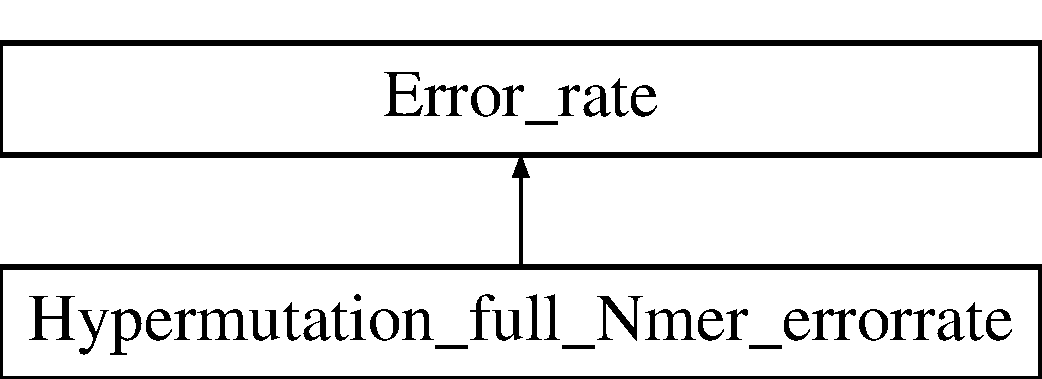
\includegraphics[height=2.000000cm]{dc/de0/classHypermutation__full__Nmer__errorrate}
\end{center}
\end{figure}
\subsection*{Public Member Functions}
\begin{DoxyCompactItemize}
\item 
\mbox{\Hypertarget{classHypermutation__full__Nmer__errorrate_ae5c78aa08882abf2ae207f291bddefc0}\label{classHypermutation__full__Nmer__errorrate_ae5c78aa08882abf2ae207f291bddefc0}} 
{\bfseries Hypermutation\+\_\+full\+\_\+\+Nmer\+\_\+errorrate} (size\+\_\+t, Gene\+\_\+class, Gene\+\_\+class, double, size\+\_\+t=0)
\item 
\mbox{\Hypertarget{classHypermutation__full__Nmer__errorrate_abf30127d93616a5a79a50997248072e5}\label{classHypermutation__full__Nmer__errorrate_abf30127d93616a5a79a50997248072e5}} 
{\bfseries Hypermutation\+\_\+full\+\_\+\+Nmer\+\_\+errorrate} (size\+\_\+t, Gene\+\_\+class, Gene\+\_\+class, std\+::vector$<$ double $>$, size\+\_\+t=0)
\item 
\mbox{\Hypertarget{classHypermutation__full__Nmer__errorrate_ab84a6d5b251ca3768312f12ef1dabb22}\label{classHypermutation__full__Nmer__errorrate_ab84a6d5b251ca3768312f12ef1dabb22}} 
{\bfseries Hypermutation\+\_\+full\+\_\+\+Nmer\+\_\+errorrate} (size\+\_\+t, Gene\+\_\+class, Gene\+\_\+class, double, std\+::string, size\+\_\+t=0)
\item 
\mbox{\Hypertarget{classHypermutation__full__Nmer__errorrate_a5d46938132c4161595c9e8262f88207a}\label{classHypermutation__full__Nmer__errorrate_a5d46938132c4161595c9e8262f88207a}} 
{\bfseries Hypermutation\+\_\+full\+\_\+\+Nmer\+\_\+errorrate} (size\+\_\+t, Gene\+\_\+class, Gene\+\_\+class, std\+::vector$<$ double $>$, std\+::string, size\+\_\+t=0)
\item 
\mbox{\Hypertarget{classHypermutation__full__Nmer__errorrate_a08bda80384e58115d3d391198b02ecca}\label{classHypermutation__full__Nmer__errorrate_a08bda80384e58115d3d391198b02ecca}} 
double {\bfseries compare\+\_\+sequences\+\_\+error\+\_\+prob} (double, const std\+::string \&, \hyperlink{classEnum__fast__memory__map}{Seq\+\_\+type\+\_\+str\+\_\+p\+\_\+map} \&, const \hyperlink{classEnum__fast__memory__dual__key__map}{Seq\+\_\+offsets\+\_\+map} \&, const std\+::unordered\+\_\+map$<$ std\+::tuple$<$ Event\+\_\+type, Gene\+\_\+class, Seq\+\_\+side $>$, std\+::shared\+\_\+ptr$<$ \hyperlink{classRec__Event}{Rec\+\_\+\+Event} $>$$>$ \&, \hyperlink{classEnum__fast__memory__map}{Mismatch\+\_\+vectors\+\_\+map} \&, double \&, double \&)
\item 
\mbox{\Hypertarget{classHypermutation__full__Nmer__errorrate_aad37473c5f4bd2a2c3a661c70dbbbb24}\label{classHypermutation__full__Nmer__errorrate_aad37473c5f4bd2a2c3a661c70dbbbb24}} 
void {\bfseries update} ()
\item 
\mbox{\Hypertarget{classHypermutation__full__Nmer__errorrate_ae3df7b9d6aa44deb4d1b3dd128d7508a}\label{classHypermutation__full__Nmer__errorrate_ae3df7b9d6aa44deb4d1b3dd128d7508a}} 
void {\bfseries initialize} (const std\+::unordered\+\_\+map$<$ std\+::tuple$<$ Event\+\_\+type, Gene\+\_\+class, Seq\+\_\+side $>$, std\+::shared\+\_\+ptr$<$ \hyperlink{classRec__Event}{Rec\+\_\+\+Event} $>$$>$ \&)
\item 
\mbox{\Hypertarget{classHypermutation__full__Nmer__errorrate_a512eb3cacde1857d68f55fdf9affed40}\label{classHypermutation__full__Nmer__errorrate_a512eb3cacde1857d68f55fdf9affed40}} 
void {\bfseries add\+\_\+to\+\_\+norm\+\_\+counter} ()
\item 
\mbox{\Hypertarget{classHypermutation__full__Nmer__errorrate_a94319d843d6064a37e20f9bdc33d7114}\label{classHypermutation__full__Nmer__errorrate_a94319d843d6064a37e20f9bdc33d7114}} 
void {\bfseries clean\+\_\+seq\+\_\+counters} ()
\item 
\mbox{\Hypertarget{classHypermutation__full__Nmer__errorrate_aa1f6aa8e6a736d4ab71a12868e1783e6}\label{classHypermutation__full__Nmer__errorrate_aa1f6aa8e6a736d4ab71a12868e1783e6}} 
void {\bfseries clean\+\_\+all\+\_\+counters} ()
\item 
\mbox{\Hypertarget{classHypermutation__full__Nmer__errorrate_a7f57702455adec179237d5cc3a9d6893}\label{classHypermutation__full__Nmer__errorrate_a7f57702455adec179237d5cc3a9d6893}} 
void {\bfseries write2txt} (std\+::ofstream \&)
\item 
\mbox{\Hypertarget{classHypermutation__full__Nmer__errorrate_a5821a0586ea2b9a793876d3c69a57379}\label{classHypermutation__full__Nmer__errorrate_a5821a0586ea2b9a793876d3c69a57379}} 
void {\bfseries set\+\_\+output\+\_\+\+Nmer\+\_\+stream} (std\+::string)
\item 
\mbox{\Hypertarget{classHypermutation__full__Nmer__errorrate_ad08335fef57c57d8b12762682c7c08fe}\label{classHypermutation__full__Nmer__errorrate_ad08335fef57c57d8b12762682c7c08fe}} 
std\+::shared\+\_\+ptr$<$ \hyperlink{classError__rate}{Error\+\_\+rate} $>$ {\bfseries copy} () const
\item 
\mbox{\Hypertarget{classHypermutation__full__Nmer__errorrate_aee43af5e346e59dcc01c732ccaae69fb}\label{classHypermutation__full__Nmer__errorrate_aee43af5e346e59dcc01c732ccaae69fb}} 
std\+::string {\bfseries type} () const
\item 
\mbox{\Hypertarget{classHypermutation__full__Nmer__errorrate_a1a7706da6d16fafe2e8846774f8ccf01}\label{classHypermutation__full__Nmer__errorrate_a1a7706da6d16fafe2e8846774f8ccf01}} 
\hyperlink{classHypermutation__full__Nmer__errorrate}{Hypermutation\+\_\+full\+\_\+\+Nmer\+\_\+errorrate} \& {\bfseries operator+=} (\hyperlink{classHypermutation__full__Nmer__errorrate}{Hypermutation\+\_\+full\+\_\+\+Nmer\+\_\+errorrate})
\item 
\mbox{\Hypertarget{classHypermutation__full__Nmer__errorrate_ae5e6673a5f849a842fd85c2aac873a06}\label{classHypermutation__full__Nmer__errorrate_ae5e6673a5f849a842fd85c2aac873a06}} 
\hyperlink{classError__rate}{Error\+\_\+rate} $\ast$ {\bfseries add\+\_\+checked} (\hyperlink{classError__rate}{Error\+\_\+rate} $\ast$)
\item 
\mbox{\Hypertarget{classHypermutation__full__Nmer__errorrate_a033630f63b43fc18b5db550fac246e6b}\label{classHypermutation__full__Nmer__errorrate_a033630f63b43fc18b5db550fac246e6b}} 
const double \& {\bfseries get\+\_\+err\+\_\+rate\+\_\+upper\+\_\+bound} (size\+\_\+t, size\+\_\+t)
\item 
\mbox{\Hypertarget{classHypermutation__full__Nmer__errorrate_a09ef2ea013441efdb25067f5e6e87c5c}\label{classHypermutation__full__Nmer__errorrate_a09ef2ea013441efdb25067f5e6e87c5c}} 
void {\bfseries build\+\_\+upper\+\_\+bound\+\_\+matrix} (size\+\_\+t, size\+\_\+t)
\item 
\mbox{\Hypertarget{classHypermutation__full__Nmer__errorrate_a84ebde8adf499035b5c6036032787da1}\label{classHypermutation__full__Nmer__errorrate_a84ebde8adf499035b5c6036032787da1}} 
int {\bfseries get\+\_\+number\+\_\+non\+\_\+zero\+\_\+likelihood\+\_\+seqs} () const
\item 
\mbox{\Hypertarget{classHypermutation__full__Nmer__errorrate_abfa7df0d953e746cdcade2d7689844d4}\label{classHypermutation__full__Nmer__errorrate_abfa7df0d953e746cdcade2d7689844d4}} 
std\+::queue$<$ int $>$ {\bfseries generate\+\_\+errors} (std\+::string \&, std\+::mt19937\+\_\+64 \&) const
\item 
\mbox{\Hypertarget{classHypermutation__full__Nmer__errorrate_a963811f5ccad25311471048896ebe7e8}\label{classHypermutation__full__Nmer__errorrate_a963811f5ccad25311471048896ebe7e8}} 
uint64\+\_\+t {\bfseries generate\+\_\+random\+\_\+mutation\+\_\+probas} (double, double)
\end{DoxyCompactItemize}
\subsection*{Additional Inherited Members}


\subsection{Detailed Description}
A non-\/additive context dependent hypermutation model. 

\begin{DoxyAuthor}{Author}
Q.\+Marcou 
\end{DoxyAuthor}
\begin{DoxyVersion}{Version}
1.\+0
\end{DoxyVersion}
A specialization of the Error\+Rate class. Implements a context dependent hypermutation/error model with tunable context size. A different mutation probability is recorded for each context of size N, leading to 4$^\wedge$N parameters. This model is inspired from the S5F mutability model. The identity of the resulting nucleotide after mutation is assumed to follow a uniform distribution. 

The documentation for this class was generated from the following files\+:\begin{DoxyCompactItemize}
\item 
Hypermutationfull\+Nmererrorrate.\+h\item 
Hypermutationfull\+Nmererrorrate.\+cpp\end{DoxyCompactItemize}

\hypertarget{classHypermutation__global__errorrate}{}\section{Hypermutation\+\_\+global\+\_\+errorrate Class Reference}
\label{classHypermutation__global__errorrate}\index{Hypermutation\+\_\+global\+\_\+errorrate@{Hypermutation\+\_\+global\+\_\+errorrate}}


An additive (independent site) context dependent hypermutation model.  




{\ttfamily \#include $<$Hypermutationglobalerrorrate.\+h$>$}

Inheritance diagram for Hypermutation\+\_\+global\+\_\+errorrate\+:\begin{figure}[H]
\begin{center}
\leavevmode
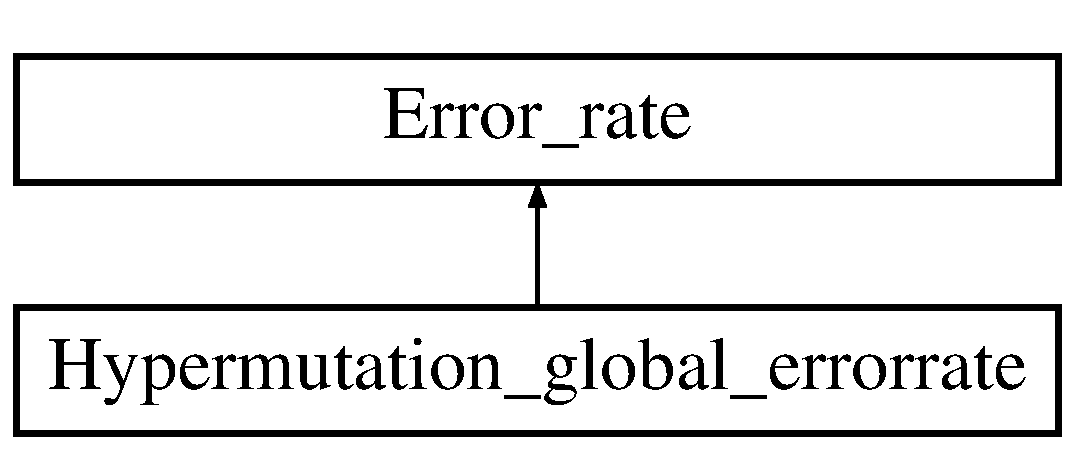
\includegraphics[height=2.000000cm]{d3/da5/classHypermutation__global__errorrate}
\end{center}
\end{figure}
\subsection*{Public Member Functions}
\begin{DoxyCompactItemize}
\item 
\mbox{\Hypertarget{classHypermutation__global__errorrate_aa99aa2d1031715691a0400609870fd12}\label{classHypermutation__global__errorrate_aa99aa2d1031715691a0400609870fd12}} 
{\bfseries Hypermutation\+\_\+global\+\_\+errorrate} (size\+\_\+t, Gene\+\_\+class, Gene\+\_\+class, double)
\item 
\mbox{\Hypertarget{classHypermutation__global__errorrate_a8446c82e50941957b918d5ffeefe54a2}\label{classHypermutation__global__errorrate_a8446c82e50941957b918d5ffeefe54a2}} 
{\bfseries Hypermutation\+\_\+global\+\_\+errorrate} (size\+\_\+t, Gene\+\_\+class, Gene\+\_\+class, double, std\+::vector$<$ double $>$)
\item 
\mbox{\Hypertarget{classHypermutation__global__errorrate_ac10eac00b3cbf526c11a3ac492a25e7d}\label{classHypermutation__global__errorrate_ac10eac00b3cbf526c11a3ac492a25e7d}} 
{\bfseries Hypermutation\+\_\+global\+\_\+errorrate} (size\+\_\+t, Gene\+\_\+class, Gene\+\_\+class, double, std\+::string)
\item 
\mbox{\Hypertarget{classHypermutation__global__errorrate_acb730ba80bd1c9e439b90350fc16a3a3}\label{classHypermutation__global__errorrate_acb730ba80bd1c9e439b90350fc16a3a3}} 
{\bfseries Hypermutation\+\_\+global\+\_\+errorrate} (size\+\_\+t, Gene\+\_\+class, Gene\+\_\+class, double, std\+::vector$<$ double $>$, std\+::string)
\item 
\mbox{\Hypertarget{classHypermutation__global__errorrate_a755458d801d03daef2f4b4f76a84df07}\label{classHypermutation__global__errorrate_a755458d801d03daef2f4b4f76a84df07}} 
double {\bfseries compare\+\_\+sequences\+\_\+error\+\_\+prob} (double, const std\+::string \&, \hyperlink{classEnum__fast__memory__map}{Seq\+\_\+type\+\_\+str\+\_\+p\+\_\+map} \&, const \hyperlink{classEnum__fast__memory__dual__key__map}{Seq\+\_\+offsets\+\_\+map} \&, const std\+::unordered\+\_\+map$<$ std\+::tuple$<$ Event\+\_\+type, Gene\+\_\+class, Seq\+\_\+side $>$, std\+::shared\+\_\+ptr$<$ \hyperlink{classRec__Event}{Rec\+\_\+\+Event} $>$$>$ \&, \hyperlink{classEnum__fast__memory__map}{Mismatch\+\_\+vectors\+\_\+map} \&, double \&, double \&)
\item 
\mbox{\Hypertarget{classHypermutation__global__errorrate_a6374b1499163375fd8b5bf76661e1230}\label{classHypermutation__global__errorrate_a6374b1499163375fd8b5bf76661e1230}} 
void {\bfseries update} ()
\item 
\mbox{\Hypertarget{classHypermutation__global__errorrate_aee8570ae02a34a718b1f0b8e8d5957f2}\label{classHypermutation__global__errorrate_aee8570ae02a34a718b1f0b8e8d5957f2}} 
void {\bfseries initialize} (const std\+::unordered\+\_\+map$<$ std\+::tuple$<$ Event\+\_\+type, Gene\+\_\+class, Seq\+\_\+side $>$, std\+::shared\+\_\+ptr$<$ \hyperlink{classRec__Event}{Rec\+\_\+\+Event} $>$$>$ \&)
\item 
\mbox{\Hypertarget{classHypermutation__global__errorrate_aa304b68d918690ef6a7332d5fc1294ef}\label{classHypermutation__global__errorrate_aa304b68d918690ef6a7332d5fc1294ef}} 
void {\bfseries add\+\_\+to\+\_\+norm\+\_\+counter} ()
\item 
\mbox{\Hypertarget{classHypermutation__global__errorrate_a5dd25d49b49187c25b88d3c4c6f90d14}\label{classHypermutation__global__errorrate_a5dd25d49b49187c25b88d3c4c6f90d14}} 
void {\bfseries clean\+\_\+seq\+\_\+counters} ()
\item 
\mbox{\Hypertarget{classHypermutation__global__errorrate_a66cc36b05f2e918e50467e624fdc5641}\label{classHypermutation__global__errorrate_a66cc36b05f2e918e50467e624fdc5641}} 
void {\bfseries clean\+\_\+all\+\_\+counters} ()
\item 
\mbox{\Hypertarget{classHypermutation__global__errorrate_a0fc0c054d923559b7e153921aff66369}\label{classHypermutation__global__errorrate_a0fc0c054d923559b7e153921aff66369}} 
void {\bfseries write2txt} (std\+::ofstream \&)
\item 
\mbox{\Hypertarget{classHypermutation__global__errorrate_ae3a5cce3c4791bd76f6bae05794604e2}\label{classHypermutation__global__errorrate_ae3a5cce3c4791bd76f6bae05794604e2}} 
void {\bfseries set\+\_\+output\+\_\+\+Nmer\+\_\+stream} (std\+::string)
\item 
\mbox{\Hypertarget{classHypermutation__global__errorrate_a5c4c403d7aefa5129cef992753d4dcce}\label{classHypermutation__global__errorrate_a5c4c403d7aefa5129cef992753d4dcce}} 
std\+::shared\+\_\+ptr$<$ \hyperlink{classError__rate}{Error\+\_\+rate} $>$ {\bfseries copy} () const
\item 
\mbox{\Hypertarget{classHypermutation__global__errorrate_a985e0277ffe8003caa5b5dcbc2c1dc80}\label{classHypermutation__global__errorrate_a985e0277ffe8003caa5b5dcbc2c1dc80}} 
std\+::string {\bfseries type} () const
\item 
\mbox{\Hypertarget{classHypermutation__global__errorrate_ae9cb6d261b6d46b5f903913debe32334}\label{classHypermutation__global__errorrate_ae9cb6d261b6d46b5f903913debe32334}} 
\hyperlink{classHypermutation__global__errorrate}{Hypermutation\+\_\+global\+\_\+errorrate} \& {\bfseries operator+=} (\hyperlink{classHypermutation__global__errorrate}{Hypermutation\+\_\+global\+\_\+errorrate})
\item 
\mbox{\Hypertarget{classHypermutation__global__errorrate_a55637ff82bc7c8c313520c6666194b99}\label{classHypermutation__global__errorrate_a55637ff82bc7c8c313520c6666194b99}} 
\hyperlink{classError__rate}{Error\+\_\+rate} $\ast$ {\bfseries add\+\_\+checked} (\hyperlink{classError__rate}{Error\+\_\+rate} $\ast$)
\item 
\mbox{\Hypertarget{classHypermutation__global__errorrate_ae99d42204a7dd7315582150f4d474353}\label{classHypermutation__global__errorrate_ae99d42204a7dd7315582150f4d474353}} 
const double \& {\bfseries get\+\_\+err\+\_\+rate\+\_\+upper\+\_\+bound} (size\+\_\+t, size\+\_\+t)
\item 
\mbox{\Hypertarget{classHypermutation__global__errorrate_ace4d25eb33bddf01dbf1e771f8997b5d}\label{classHypermutation__global__errorrate_ace4d25eb33bddf01dbf1e771f8997b5d}} 
void {\bfseries build\+\_\+upper\+\_\+bound\+\_\+matrix} (size\+\_\+t, size\+\_\+t)
\item 
\mbox{\Hypertarget{classHypermutation__global__errorrate_a7ae06e4aa431aefc2386a74939778c10}\label{classHypermutation__global__errorrate_a7ae06e4aa431aefc2386a74939778c10}} 
int {\bfseries get\+\_\+number\+\_\+non\+\_\+zero\+\_\+likelihood\+\_\+seqs} () const
\item 
\mbox{\Hypertarget{classHypermutation__global__errorrate_a4783b1ad113de7c77712c996ff0a1b3c}\label{classHypermutation__global__errorrate_a4783b1ad113de7c77712c996ff0a1b3c}} 
std\+::queue$<$ int $>$ {\bfseries generate\+\_\+errors} (std\+::string \&, std\+::mt19937\+\_\+64 \&) const
\item 
\mbox{\Hypertarget{classHypermutation__global__errorrate_a10b75cea037da01947037a74b86a5653}\label{classHypermutation__global__errorrate_a10b75cea037da01947037a74b86a5653}} 
uint64\+\_\+t {\bfseries generate\+\_\+random\+\_\+contributions} (double)
\end{DoxyCompactItemize}
\subsection*{Additional Inherited Members}


\subsection{Detailed Description}
An additive (independent site) context dependent hypermutation model. 

\begin{DoxyAuthor}{Author}
Q.\+Marcou 
\end{DoxyAuthor}
\begin{DoxyVersion}{Version}
1.\+0
\end{DoxyVersion}
A specialization of the Error\+Rate class. Implements a context dependent hypermutation/error model with tunable context size. Nucleotide from the context are assumed to contribute independently to the mutability of the context through an additive logarithmic score. Such a model contains only 3\+N+1 parameters and allows to probe large context sizes. The identity of the resulting nucleotide after mutation is assumed to follow a uniform distribution. 

The documentation for this class was generated from the following files\+:\begin{DoxyCompactItemize}
\item 
Hypermutationglobalerrorrate.\+h\item 
Hypermutationglobalerrorrate.\+cpp\end{DoxyCompactItemize}

\hypertarget{classInsertion}{}\section{Insertion Class Reference}
\label{classInsertion}\index{Insertion@{Insertion}}


\hyperlink{classInsertion}{Insertion} recombination events.  




{\ttfamily \#include $<$Insertion.\+h$>$}

Inheritance diagram for Insertion\+:\begin{figure}[H]
\begin{center}
\leavevmode
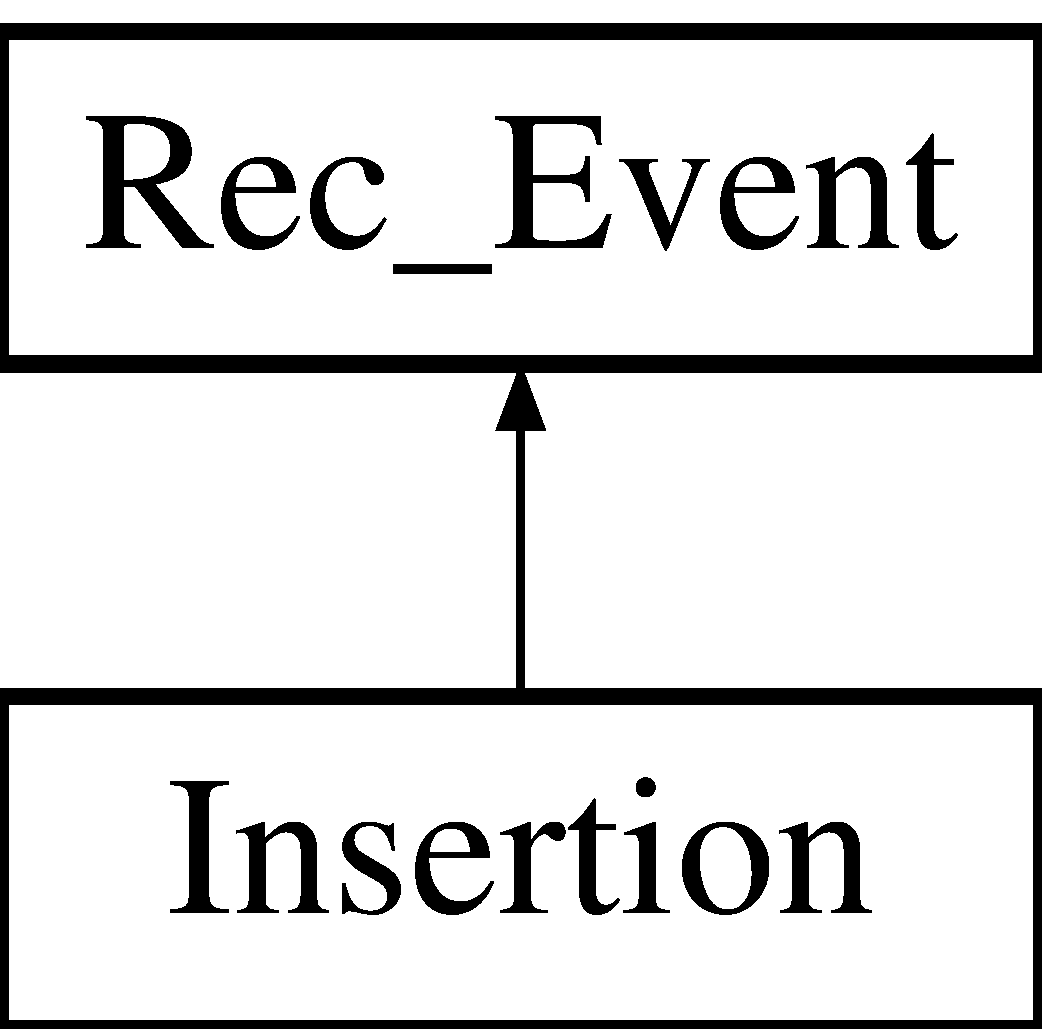
\includegraphics[height=2.000000cm]{d1/d70/classInsertion}
\end{center}
\end{figure}
\subsection*{Public Member Functions}
\begin{DoxyCompactItemize}
\item 
\mbox{\Hypertarget{classInsertion_a0d34760832ea7f19cbac094a242d0e28}\label{classInsertion_a0d34760832ea7f19cbac094a242d0e28}} 
{\bfseries Insertion} (Gene\+\_\+class, std\+::pair$<$ int, int $>$)
\item 
\mbox{\Hypertarget{classInsertion_a0fac0c59a950d2b9a0f4665dea103b5f}\label{classInsertion_a0fac0c59a950d2b9a0f4665dea103b5f}} 
{\bfseries Insertion} (Gene\+\_\+class, std\+::forward\+\_\+list$<$ int $>$)
\item 
\mbox{\Hypertarget{classInsertion_ad50ab30acaa070dafc9856804cee7191}\label{classInsertion_ad50ab30acaa070dafc9856804cee7191}} 
{\bfseries Insertion} (Gene\+\_\+class)
\item 
\mbox{\Hypertarget{classInsertion_a21d1cf32f7cb2505ace6560499af6ff0}\label{classInsertion_a21d1cf32f7cb2505ace6560499af6ff0}} 
{\bfseries Insertion} (Gene\+\_\+class, std\+::unordered\+\_\+map$<$ std\+::string, \hyperlink{structEvent__realization}{Event\+\_\+realization} $>$ \&)
\item 
\mbox{\Hypertarget{classInsertion_a4d3b461170165250720e8a237c56be07}\label{classInsertion_a4d3b461170165250720e8a237c56be07}} 
std\+::shared\+\_\+ptr$<$ \hyperlink{classRec__Event}{Rec\+\_\+\+Event} $>$ {\bfseries copy} ()
\item 
void \hyperlink{classInsertion_a9c0f15989a298d7ddf7311c432f995b9}{iterate} (double \&, \hyperlink{classEnum__fast__memory__map}{Downstream\+\_\+scenario\+\_\+proba\+\_\+bound\+\_\+map} \&, const std\+::string \&, const \hyperlink{classInt__Str}{Int\+\_\+\+Str} \&, \hyperlink{classEnum__fast__memory__map}{Index\+\_\+map} \&, const std\+::unordered\+\_\+map$<$ Rec\+\_\+\+Event\+\_\+name, std\+::vector$<$ std\+::pair$<$ std\+::shared\+\_\+ptr$<$ const \hyperlink{classRec__Event}{Rec\+\_\+\+Event} $>$, int $>$$>$$>$ \&, std\+::shared\+\_\+ptr$<$ \hyperlink{classRec__Event}{Next\+\_\+event\+\_\+ptr} $>$ \&, Marginal\+\_\+array\+\_\+p \&, const Marginal\+\_\+array\+\_\+p \&, const std\+::unordered\+\_\+map$<$ Gene\+\_\+class, std\+::vector$<$ \hyperlink{structAlignment__data}{Alignment\+\_\+data} $>$$>$ \&, \hyperlink{classEnum__fast__memory__map}{Seq\+\_\+type\+\_\+str\+\_\+p\+\_\+map} \&, \hyperlink{classEnum__fast__memory__dual__key__map}{Seq\+\_\+offsets\+\_\+map} \&, std\+::shared\+\_\+ptr$<$ \hyperlink{classError__rate}{Error\+\_\+rate} $>$ \&, std\+::map$<$ size\+\_\+t, std\+::shared\+\_\+ptr$<$ \hyperlink{classCounter}{Counter} $>$$>$ \&, const std\+::unordered\+\_\+map$<$ std\+::tuple$<$ Event\+\_\+type, Gene\+\_\+class, Seq\+\_\+side $>$, std\+::shared\+\_\+ptr$<$ \hyperlink{classRec__Event}{Rec\+\_\+\+Event} $>$$>$ \&, \hyperlink{classEnum__fast__memory__map}{Safety\+\_\+bool\+\_\+map} \&, \hyperlink{classEnum__fast__memory__map}{Mismatch\+\_\+vectors\+\_\+map} \&, double \&, double \&)
\begin{DoxyCompactList}\small\item\em Evaluate all Event\+\_\+\+Realization of a Rec\+Event for a given sequence. \end{DoxyCompactList}\item 
\mbox{\Hypertarget{classInsertion_abb12662317d803931ca241d68fdfeb58}\label{classInsertion_abb12662317d803931ca241d68fdfeb58}} 
bool {\bfseries add\+\_\+realization} (int)
\item 
\mbox{\Hypertarget{classInsertion_a3411f67c94b8c44b5238c48ec8f9d035}\label{classInsertion_a3411f67c94b8c44b5238c48ec8f9d035}} 
std\+::queue$<$ int $>$ {\bfseries draw\+\_\+random\+\_\+realization} (const Marginal\+\_\+array\+\_\+p \&, std\+::unordered\+\_\+map$<$ Rec\+\_\+\+Event\+\_\+name, int $>$ \&, const std\+::unordered\+\_\+map$<$ Rec\+\_\+\+Event\+\_\+name, std\+::vector$<$ std\+::pair$<$ std\+::shared\+\_\+ptr$<$ const \hyperlink{classRec__Event}{Rec\+\_\+\+Event} $>$, int $>$$>$$>$ \&, std\+::unordered\+\_\+map$<$ Seq\+\_\+type, std\+::string $>$ \&, std\+::mt19937\+\_\+64 \&) const
\item 
\mbox{\Hypertarget{classInsertion_a30b42a3588251fa54d4c59da67493ed9}\label{classInsertion_a30b42a3588251fa54d4c59da67493ed9}} 
void {\bfseries write2txt} (std\+::ofstream \&)
\item 
\mbox{\Hypertarget{classInsertion_a249374ebfac39b6f413af9d240bf69f2}\label{classInsertion_a249374ebfac39b6f413af9d240bf69f2}} 
void {\bfseries initialize\+\_\+event} (std\+::unordered\+\_\+set$<$ Rec\+\_\+\+Event\+\_\+name $>$ \&, const std\+::unordered\+\_\+map$<$ std\+::tuple$<$ Event\+\_\+type, Gene\+\_\+class, Seq\+\_\+side $>$, std\+::shared\+\_\+ptr$<$ \hyperlink{classRec__Event}{Rec\+\_\+\+Event} $>$$>$ \&, const std\+::unordered\+\_\+map$<$ Rec\+\_\+\+Event\+\_\+name, std\+::vector$<$ std\+::pair$<$ std\+::shared\+\_\+ptr$<$ const \hyperlink{classRec__Event}{Rec\+\_\+\+Event} $>$, int $>$$>$$>$ \&, \hyperlink{classEnum__fast__memory__map}{Downstream\+\_\+scenario\+\_\+proba\+\_\+bound\+\_\+map} \&, \hyperlink{classEnum__fast__memory__map}{Seq\+\_\+type\+\_\+str\+\_\+p\+\_\+map} \&, \hyperlink{classEnum__fast__memory__map}{Safety\+\_\+bool\+\_\+map} \&, std\+::shared\+\_\+ptr$<$ \hyperlink{classError__rate}{Error\+\_\+rate} $>$, \hyperlink{classEnum__fast__memory__map}{Mismatch\+\_\+vectors\+\_\+map} \&, \hyperlink{classEnum__fast__memory__dual__key__map}{Seq\+\_\+offsets\+\_\+map} \&, \hyperlink{classEnum__fast__memory__map}{Index\+\_\+map} \&)
\item 
\mbox{\Hypertarget{classInsertion_a139905cff68908afdc55ee9fabafb191}\label{classInsertion_a139905cff68908afdc55ee9fabafb191}} 
void {\bfseries add\+\_\+to\+\_\+marginals} (long double, Marginal\+\_\+array\+\_\+p \&) const
\item 
\mbox{\Hypertarget{classInsertion_a5c38b8caabad0eda4f948410fd863a37}\label{classInsertion_a5c38b8caabad0eda4f948410fd863a37}} 
void {\bfseries set\+\_\+crude\+\_\+upper\+\_\+bound\+\_\+proba} (size\+\_\+t, size\+\_\+t, Marginal\+\_\+array\+\_\+p \&)
\item 
\mbox{\Hypertarget{classInsertion_aa23f4e5196c4993419f0dbe73142704c}\label{classInsertion_aa23f4e5196c4993419f0dbe73142704c}} 
void {\bfseries initialize\+\_\+crude\+\_\+scenario\+\_\+proba\+\_\+bound} (double \&, std\+::forward\+\_\+list$<$ double $\ast$$>$ \&, const std\+::unordered\+\_\+map$<$ std\+::tuple$<$ Event\+\_\+type, Gene\+\_\+class, Seq\+\_\+side $>$, std\+::shared\+\_\+ptr$<$ \hyperlink{classRec__Event}{Rec\+\_\+\+Event} $>$$>$ \&)
\item 
\mbox{\Hypertarget{classInsertion_ab050d5c2cc7a609c0ab519f9af7a3eca}\label{classInsertion_ab050d5c2cc7a609c0ab519f9af7a3eca}} 
bool {\bfseries has\+\_\+effect\+\_\+on} (Seq\+\_\+type) const
\item 
\mbox{\Hypertarget{classInsertion_a220705a85efcbca8085e31495d6cefdb}\label{classInsertion_a220705a85efcbca8085e31495d6cefdb}} 
void {\bfseries iterate\+\_\+initialize\+\_\+\+Len\+\_\+proba} (Seq\+\_\+type considered\+\_\+junction, std\+::map$<$ int, double $>$ \&length\+\_\+best\+\_\+proba\+\_\+map, std\+::queue$<$ std\+::shared\+\_\+ptr$<$ \hyperlink{classRec__Event}{Rec\+\_\+\+Event} $>$$>$ \&model\+\_\+queue, double \&scenario\+\_\+proba, const Marginal\+\_\+array\+\_\+p \&model\+\_\+parameters\+\_\+point, \hyperlink{classEnum__fast__memory__map}{Index\+\_\+map} \&base\+\_\+index\+\_\+map, \hyperlink{classEnum__fast__memory__map}{Seq\+\_\+type\+\_\+str\+\_\+p\+\_\+map} \&constructed\+\_\+sequences, int \&seq\+\_\+len) const
\item 
\mbox{\Hypertarget{classInsertion_a3e0b4b03bdfe363c630f7b5012165650}\label{classInsertion_a3e0b4b03bdfe363c630f7b5012165650}} 
void {\bfseries initialize\+\_\+\+Len\+\_\+proba\+\_\+bound} (std\+::queue$<$ std\+::shared\+\_\+ptr$<$ \hyperlink{classRec__Event}{Rec\+\_\+\+Event} $>$$>$ \&model\+\_\+queue, const Marginal\+\_\+array\+\_\+p \&model\+\_\+parameters\+\_\+point, \hyperlink{classEnum__fast__memory__map}{Index\+\_\+map} \&base\+\_\+index\+\_\+map)
\end{DoxyCompactItemize}
\subsection*{Additional Inherited Members}


\subsection{Detailed Description}
\hyperlink{classInsertion}{Insertion} recombination events. 

\begin{DoxyAuthor}{Author}
Q.\+Marcou 
\end{DoxyAuthor}
\begin{DoxyVersion}{Version}
1.\+0
\end{DoxyVersion}
The \hyperlink{classInsertion}{Insertion} Rec\+Event models the distribution of junctional insertion length during the V(\+D)J recombination process. 

\subsection{Member Function Documentation}
\mbox{\Hypertarget{classInsertion_a9c0f15989a298d7ddf7311c432f995b9}\label{classInsertion_a9c0f15989a298d7ddf7311c432f995b9}} 
\index{Insertion@{Insertion}!iterate@{iterate}}
\index{iterate@{iterate}!Insertion@{Insertion}}
\subsubsection{\texorpdfstring{iterate()}{iterate()}}
{\footnotesize\ttfamily void Insertion\+::iterate (\begin{DoxyParamCaption}\item[{double \&}]{,  }\item[{\hyperlink{classEnum__fast__memory__map}{Downstream\+\_\+scenario\+\_\+proba\+\_\+bound\+\_\+map} \&}]{,  }\item[{const std\+::string \&}]{,  }\item[{const \hyperlink{classInt__Str}{Int\+\_\+\+Str} \&}]{,  }\item[{\hyperlink{classEnum__fast__memory__map}{Index\+\_\+map} \&}]{,  }\item[{const std\+::unordered\+\_\+map$<$ Rec\+\_\+\+Event\+\_\+name, std\+::vector$<$ std\+::pair$<$ std\+::shared\+\_\+ptr$<$ const \hyperlink{classRec__Event}{Rec\+\_\+\+Event} $>$, int $>$$>$$>$ \&}]{,  }\item[{std\+::shared\+\_\+ptr$<$ \hyperlink{classRec__Event}{Next\+\_\+event\+\_\+ptr} $>$ \&}]{,  }\item[{Marginal\+\_\+array\+\_\+p \&}]{,  }\item[{const Marginal\+\_\+array\+\_\+p \&}]{,  }\item[{const std\+::unordered\+\_\+map$<$ Gene\+\_\+class, std\+::vector$<$ \hyperlink{structAlignment__data}{Alignment\+\_\+data} $>$$>$ \&}]{,  }\item[{\hyperlink{classEnum__fast__memory__map}{Seq\+\_\+type\+\_\+str\+\_\+p\+\_\+map} \&}]{,  }\item[{\hyperlink{classEnum__fast__memory__dual__key__map}{Seq\+\_\+offsets\+\_\+map} \&}]{,  }\item[{std\+::shared\+\_\+ptr$<$ \hyperlink{classError__rate}{Error\+\_\+rate} $>$ \&}]{,  }\item[{std\+::map$<$ size\+\_\+t, std\+::shared\+\_\+ptr$<$ \hyperlink{classCounter}{Counter} $>$$>$ \&}]{,  }\item[{const std\+::unordered\+\_\+map$<$ std\+::tuple$<$ Event\+\_\+type, Gene\+\_\+class, Seq\+\_\+side $>$, std\+::shared\+\_\+ptr$<$ \hyperlink{classRec__Event}{Rec\+\_\+\+Event} $>$$>$ \&}]{,  }\item[{\hyperlink{classEnum__fast__memory__map}{Safety\+\_\+bool\+\_\+map} \&}]{,  }\item[{\hyperlink{classEnum__fast__memory__map}{Mismatch\+\_\+vectors\+\_\+map} \&}]{,  }\item[{double \&}]{,  }\item[{double \&}]{ }\end{DoxyParamCaption})\hspace{0.3cm}{\ttfamily [inline]}, {\ttfamily [virtual]}}



Evaluate all Event\+\_\+\+Realization of a Rec\+Event for a given sequence. 

\begin{DoxyAuthor}{Author}
Q.\+Marcou 
\end{DoxyAuthor}
\begin{DoxyVersion}{Version}
1.\+0 
\end{DoxyVersion}

\begin{DoxyParams}[1]{Parameters}
\mbox{\tt in,out}  & {\em scenario\+\_\+proba} & Probability of the currently explored (incomplete) scenario \\
\hline
\mbox{\tt in,out}  & {\em downstream\+\_\+proba\+\_\+map} & \\
\hline
\mbox{\tt in}  & {\em sequence} & The studied sequence in nucleotide code \\
\hline
\mbox{\tt in}  & {\em int\+\_\+sequence} & The studied sequence in integer code \\
\hline
\mbox{\tt in,out}  & {\em base\+\_\+index\+\_\+map} & Dynamic map recording where probabilities should be read on the marginals. \\
\hline
\mbox{\tt in}  & {\em offset\+\_\+map} & Tells the event by how much indices from the children events should be modified \\
\hline
\mbox{\tt in}  & {\em next\+\_\+event\+\_\+ptr\+\_\+arr} & Indicates the next event to call iterate on \\
\hline
\mbox{\tt in}  & {\em updated\+\_\+marginals\+\_\+point} & Summary marginals on which complete scenario posteriors are recorded \\
\hline
\mbox{\tt in}  & {\em model\+\_\+parameters\+\_\+point} & Current recombination probability distribution \\
\hline
\mbox{\tt in}  & {\em allowed\+\_\+realizations} & The set of genomic templates alignment \\
\hline
\mbox{\tt in,out}  & {\em constructed\+\_\+sequences} & Map containing the (incomplete) scenario\textquotesingle{}s resulting sequence \\
\hline
\mbox{\tt in,out}  & {\em seq\+\_\+offsets} & Map containing the 3\textquotesingle{} and 5\textquotesingle{} offsets of each scenario sequence piece \\
\hline
\mbox{\tt in}  & {\em error\+\_\+rate\+\_\+p} & Pointer to the error model object \\
\hline
\mbox{\tt in}  & {\em counters\+\_\+list} & The list of \hyperlink{classCounter}{Counter} to be counted \\
\hline
\mbox{\tt in}  & {\em events\+\_\+map} & A map containing all events contained in the Model\+\_\+parms, accessible through their type, gene class and side. \\
\hline
\mbox{\tt in,out}  & {\em safety\+\_\+set} & A map indicating whether checks on offsets overlap should be performed \\
\hline
\mbox{\tt in,out}  & {\em mismatches\+\_\+lists} & A map containing the (incomplete) scenario mismatches \\
\hline
\mbox{\tt in}  & {\em seq\+\_\+max\+\_\+prob\+\_\+scenario} & Most likely scenario\textquotesingle{}s probability for the considered sequence \\
\hline
\mbox{\tt in}  & {\em proba\+\_\+threshold\+\_\+factor} & Threshold on probability ratio between most likely scenario and explored scenario\\
\hline
\end{DoxyParams}
\begin{DoxyReturn}{Returns}
void
\end{DoxyReturn}
The iterate method is the heart of I\+GoR\textquotesingle{}s scenario exploration. \hyperlink{classModel__Parms}{Model\+\_\+\+Parms} define an order in which the Rec\+Event should be processed. Upon call of iterate all Event\+Realization of the Rec\+Event are assessed and for each possible realization the iterate method is called recursively for the next event. Inside the iterate method a filtering on too improbable realizations is performed (tree prunning) using the downstream\+\_\+proba\+\_\+map.

The index map is used to read off the probability of the current Rec\+Event Event\+Realization at the correct location given the events parent\textquotesingle{}s realizations. It is further modified to take into account the current event\textquotesingle{}s realization when its children realization probabilities will be read. 

Implements \hyperlink{classRec__Event_a0fea607ec06bdd1a7f5ebb04a96e5253}{Rec\+\_\+\+Event}.



The documentation for this class was generated from the following files\+:\begin{DoxyCompactItemize}
\item 
Insertion.\+h\item 
Insertion.\+cpp\end{DoxyCompactItemize}

\hypertarget{classInt__Str}{}\section{Int\+\_\+\+Str Class Reference}
\label{classInt__Str}\index{Int\+\_\+\+Str@{Int\+\_\+\+Str}}
Inheritance diagram for Int\+\_\+\+Str\+:\begin{figure}[H]
\begin{center}
\leavevmode
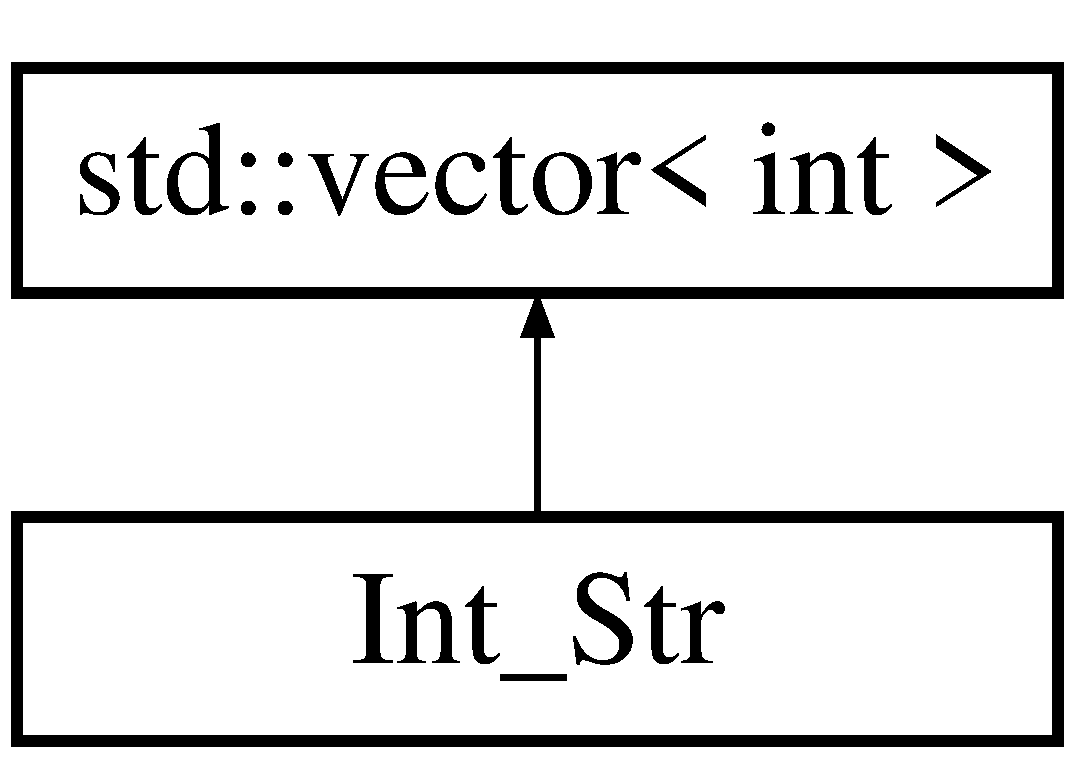
\includegraphics[height=2.000000cm]{df/d59/classInt__Str}
\end{center}
\end{figure}
\subsection*{Public Member Functions}
\begin{DoxyCompactItemize}
\item 
\mbox{\Hypertarget{classInt__Str_a60811d3005bed5b04f07d9e76725585f}\label{classInt__Str_a60811d3005bed5b04f07d9e76725585f}} 
\hyperlink{classInt__Str}{Int\+\_\+\+Str} \& {\bfseries operator+=} (const \hyperlink{classInt__Str}{Int\+\_\+\+Str} \&)
\item 
\mbox{\Hypertarget{classInt__Str_a59a0385a61b301237ce2867534a874d3}\label{classInt__Str_a59a0385a61b301237ce2867534a874d3}} 
\hyperlink{classInt__Str}{Int\+\_\+\+Str} \& {\bfseries operator+=} (const int \&)
\item 
\mbox{\Hypertarget{classInt__Str_a479979830665bac8db3faaa6bbc5d757}\label{classInt__Str_a479979830665bac8db3faaa6bbc5d757}} 
\hyperlink{classInt__Str}{Int\+\_\+\+Str} \& {\bfseries operator+=} (int \&\&)
\item 
\mbox{\Hypertarget{classInt__Str_ae8ab9c74d87a9d57aa05d307595f28ed}\label{classInt__Str_ae8ab9c74d87a9d57aa05d307595f28ed}} 
\hyperlink{classInt__Str}{Int\+\_\+\+Str} \& {\bfseries append} (const \hyperlink{classInt__Str}{Int\+\_\+\+Str} \&)
\item 
\mbox{\Hypertarget{classInt__Str_a40f839f59804aebc4465a07790a14145}\label{classInt__Str_a40f839f59804aebc4465a07790a14145}} 
\hyperlink{classInt__Str}{Int\+\_\+\+Str} \& {\bfseries append} (const int \&)
\item 
\mbox{\Hypertarget{classInt__Str_a9c5eac2de96578033443396b1e5096b8}\label{classInt__Str_a9c5eac2de96578033443396b1e5096b8}} 
\hyperlink{classInt__Str}{Int\+\_\+\+Str} {\bfseries operator+} (const \hyperlink{classInt__Str}{Int\+\_\+\+Str} \&) const
\item 
\mbox{\Hypertarget{classInt__Str_ac3464ca7854d86178a90cfa72aeaa064}\label{classInt__Str_ac3464ca7854d86178a90cfa72aeaa064}} 
\hyperlink{classInt__Str}{Int\+\_\+\+Str} {\bfseries operator+} (const int \&) const
\item 
\mbox{\Hypertarget{classInt__Str_aeba1b1ef0ff0302da41547bfeaada690}\label{classInt__Str_aeba1b1ef0ff0302da41547bfeaada690}} 
\hyperlink{classInt__Str}{Int\+\_\+\+Str} {\bfseries operator+} (int) const
\item 
\mbox{\Hypertarget{classInt__Str_afdda294e03fc043c89efd9bbaa130fee}\label{classInt__Str_afdda294e03fc043c89efd9bbaa130fee}} 
\hyperlink{classInt__Str}{Int\+\_\+\+Str} {\bfseries substr} (std\+::size\+\_\+t pos=0, std\+::size\+\_\+t len=npos) const
\item 
\mbox{\Hypertarget{classInt__Str_a229a4463cc501ed64f0796513341fa64}\label{classInt__Str_a229a4463cc501ed64f0796513341fa64}} 
\hyperlink{classInt__Str}{Int\+\_\+\+Str} \& {\bfseries erase} (std\+::size\+\_\+t pos, std\+::size\+\_\+t len)
\end{DoxyCompactItemize}
\subsection*{Static Public Attributes}
\begin{DoxyCompactItemize}
\item 
\mbox{\Hypertarget{classInt__Str_ae168eec8cfc26ee125a8daf7ea2b434b}\label{classInt__Str_ae168eec8cfc26ee125a8daf7ea2b434b}} 
static const std\+::size\+\_\+t {\bfseries npos} = -\/1
\end{DoxyCompactItemize}


The documentation for this class was generated from the following files\+:\begin{DoxyCompactItemize}
\item 
Int\+Str.\+h\item 
Int\+Str.\+cpp\end{DoxyCompactItemize}

\hypertarget{structinverse__offset__comparator}{}\section{inverse\+\_\+offset\+\_\+comparator Struct Reference}
\label{structinverse__offset__comparator}\index{inverse\+\_\+offset\+\_\+comparator@{inverse\+\_\+offset\+\_\+comparator}}
\subsection*{Public Member Functions}
\begin{DoxyCompactItemize}
\item 
\mbox{\Hypertarget{structinverse__offset__comparator_afa8f3857c10adb3cd7f7cdb4b0cedc64}\label{structinverse__offset__comparator_afa8f3857c10adb3cd7f7cdb4b0cedc64}} 
bool {\bfseries operator()} (const std\+::pair$<$ std\+::shared\+\_\+ptr$<$ const \hyperlink{classRec__Event}{Rec\+\_\+\+Event} $>$, int $>$ \&inv\+\_\+offset\+\_\+1, const std\+::pair$<$ std\+::shared\+\_\+ptr$<$ const \hyperlink{classRec__Event}{Rec\+\_\+\+Event} $>$, int $>$ \&inv\+\_\+offset\+\_\+2)
\end{DoxyCompactItemize}


The documentation for this struct was generated from the following file\+:\begin{DoxyCompactItemize}
\item 
Utils.\+h\end{DoxyCompactItemize}

\hypertarget{structMatrix}{}\section{Matrix$<$ T $>$ Struct Template Reference}
\label{structMatrix}\index{Matrix$<$ T $>$@{Matrix$<$ T $>$}}
\subsection*{Public Member Functions}
\begin{DoxyCompactItemize}
\item 
\mbox{\Hypertarget{structMatrix_ab214150a26c19a3f66fba2a7dab86d04}\label{structMatrix_ab214150a26c19a3f66fba2a7dab86d04}} 
{\bfseries Matrix} (int m, int n)
\item 
\mbox{\Hypertarget{structMatrix_a235ed010302613a018fffc144f3e6fc6}\label{structMatrix_a235ed010302613a018fffc144f3e6fc6}} 
{\bfseries Matrix} (int m, int n, T arr\mbox{[}$\,$\mbox{]})
\item 
\mbox{\Hypertarget{structMatrix_ae68125e7246979d0f2103cef913c3135}\label{structMatrix_ae68125e7246979d0f2103cef913c3135}} 
{\bfseries Matrix} (int m, int n, std\+::vector$<$ T $>$ vect)
\item 
\mbox{\Hypertarget{structMatrix_a1012080b9cf91044d58c11f5a49c8230}\label{structMatrix_a1012080b9cf91044d58c11f5a49c8230}} 
{\bfseries Matrix} (const \hyperlink{structMatrix}{Matrix}$<$ T $>$ \&other)
\item 
\mbox{\Hypertarget{structMatrix_ab688e0d1d2c4ad2cb04262f3a056d902}\label{structMatrix_ab688e0d1d2c4ad2cb04262f3a056d902}} 
\hyperlink{structMatrix}{Matrix}$<$ T $>$ \& {\bfseries operator=} (const \hyperlink{structMatrix}{Matrix} \&other)
\item 
\mbox{\Hypertarget{structMatrix_a1a09c4488e6db5901b7f6c5de327d8bf}\label{structMatrix_a1a09c4488e6db5901b7f6c5de327d8bf}} 
T \& {\bfseries operator()} (const int \&i, const int \&j)
\item 
\mbox{\Hypertarget{structMatrix_ac4d46c6bf2be24bf4bcea7ae47c5e814}\label{structMatrix_ac4d46c6bf2be24bf4bcea7ae47c5e814}} 
const T \& {\bfseries operator()} (const int \&i, const int \&j) const
\item 
\mbox{\Hypertarget{structMatrix_adb3acce57a0e471129700f61479322eb}\label{structMatrix_adb3acce57a0e471129700f61479322eb}} 
T {\bfseries get\+\_\+field} (const int \&i, const int \&j) const
\item 
\mbox{\Hypertarget{structMatrix_a9aaa59e7e0355a6d2eeed105f5314b72}\label{structMatrix_a9aaa59e7e0355a6d2eeed105f5314b72}} 
const int \& {\bfseries get\+\_\+n\+\_\+rows} () const
\item 
\mbox{\Hypertarget{structMatrix_acf8cc1fcc08d41a9eb68055b5feb99b4}\label{structMatrix_acf8cc1fcc08d41a9eb68055b5feb99b4}} 
const int \& {\bfseries get\+\_\+n\+\_\+cols} () const
\end{DoxyCompactItemize}


The documentation for this struct was generated from the following file\+:\begin{DoxyCompactItemize}
\item 
Utils.\+h\end{DoxyCompactItemize}

\hypertarget{classModel__marginals}{}\section{Model\+\_\+marginals Class Reference}
\label{classModel__marginals}\index{Model\+\_\+marginals@{Model\+\_\+marginals}}


Encapsulates the marginal probabilities/posterior frequency for each recombination event\textquotesingle{}s realization.  




{\ttfamily \#include $<$Model\+\_\+marginals.\+h$>$}

\subsection*{Public Member Functions}
\begin{DoxyCompactItemize}
\item 
\mbox{\Hypertarget{classModel__marginals_af39c167e148333d7ef0fbb7e3671e4e6}\label{classModel__marginals_af39c167e148333d7ef0fbb7e3671e4e6}} 
{\bfseries Model\+\_\+marginals} (const \hyperlink{classModel__Parms}{Model\+\_\+\+Parms} \&)
\item 
\mbox{\Hypertarget{classModel__marginals_a8940e4e8b183b0a9cc7678dc1c3aac69}\label{classModel__marginals_a8940e4e8b183b0a9cc7678dc1c3aac69}} 
{\bfseries Model\+\_\+marginals} (const \hyperlink{classModel__marginals}{Model\+\_\+marginals} \&)
\item 
\mbox{\Hypertarget{classModel__marginals_abc7cf626d915e7a6a9805b3d2a9e6ddf}\label{classModel__marginals_abc7cf626d915e7a6a9805b3d2a9e6ddf}} 
size\+\_\+t {\bfseries compute\+\_\+size} (const \hyperlink{classModel__Parms}{Model\+\_\+\+Parms} \&)
\item 
\mbox{\Hypertarget{classModel__marginals_a97ee1d30aa7638a1a1c3e4362ded1fe4}\label{classModel__marginals_a97ee1d30aa7638a1a1c3e4362ded1fe4}} 
size\+\_\+t {\bfseries get\+\_\+event\+\_\+size} (std\+::shared\+\_\+ptr$<$ const \hyperlink{classRec__Event}{Rec\+\_\+\+Event} $>$, const \hyperlink{classModel__Parms}{Model\+\_\+\+Parms} \&) const
\item 
\mbox{\Hypertarget{classModel__marginals_ae4ef378bbec817842572b5538e95899e}\label{classModel__marginals_ae4ef378bbec817842572b5538e95899e}} 
std\+::pair$<$ std\+::list$<$ std\+::pair$<$ Rec\+\_\+\+Event\+\_\+name, size\+\_\+t $>$ $>$, std\+::shared\+\_\+ptr$<$ long double $>$ $>$ {\bfseries compute\+\_\+event\+\_\+marginal\+\_\+probability} (Rec\+\_\+\+Event\+\_\+name, const \hyperlink{classModel__Parms}{Model\+\_\+\+Parms} \&) const
\item 
\mbox{\Hypertarget{classModel__marginals_a2e60c477a567ee76de8f0e7ec6929364}\label{classModel__marginals_a2e60c477a567ee76de8f0e7ec6929364}} 
std\+::pair$<$ std\+::list$<$ std\+::pair$<$ Rec\+\_\+\+Event\+\_\+name, size\+\_\+t $>$ $>$, std\+::shared\+\_\+ptr$<$ long double $>$ $>$ {\bfseries compute\+\_\+event\+\_\+marginal\+\_\+probability} (Rec\+\_\+\+Event\+\_\+name, const std\+::set$<$ Rec\+\_\+\+Event\+\_\+name $>$ \&, const \hyperlink{classModel__Parms}{Model\+\_\+\+Parms} \&) const
\item 
\mbox{\Hypertarget{classModel__marginals_a9791d1f5adb5a336b02b39129618990a}\label{classModel__marginals_a9791d1f5adb5a336b02b39129618990a}} 
\hyperlink{classModel__marginals}{Model\+\_\+marginals} \& {\bfseries operator=} (const \hyperlink{classModel__marginals}{Model\+\_\+marginals} \&)
\item 
\mbox{\Hypertarget{classModel__marginals_a2dd9431c456a5f3d74b3882cb0754daf}\label{classModel__marginals_a2dd9431c456a5f3d74b3882cb0754daf}} 
\hyperlink{classModel__marginals}{Model\+\_\+marginals} \& {\bfseries operator+=} (\hyperlink{classModel__marginals}{Model\+\_\+marginals})
\item 
\mbox{\Hypertarget{classModel__marginals_aff98fb8317f93d4cac83b1c0e95139dd}\label{classModel__marginals_aff98fb8317f93d4cac83b1c0e95139dd}} 
\hyperlink{classModel__marginals}{Model\+\_\+marginals} \& {\bfseries operator-\/=} (\hyperlink{classModel__marginals}{Model\+\_\+marginals})
\item 
\mbox{\Hypertarget{classModel__marginals_a349fc9203c44d78b412128f182edf3be}\label{classModel__marginals_a349fc9203c44d78b412128f182edf3be}} 
\hyperlink{classModel__marginals}{Model\+\_\+marginals} {\bfseries operator+} (\hyperlink{classModel__marginals}{Model\+\_\+marginals})
\item 
\mbox{\Hypertarget{classModel__marginals_aa5f6720c88c804180bfcd3e433efb7ad}\label{classModel__marginals_aa5f6720c88c804180bfcd3e433efb7ad}} 
\hyperlink{classModel__marginals}{Model\+\_\+marginals} {\bfseries operator-\/} (\hyperlink{classModel__marginals}{Model\+\_\+marginals})
\item 
\mbox{\Hypertarget{classModel__marginals_afcfcba336f58b08e37074556b82650e8}\label{classModel__marginals_afcfcba336f58b08e37074556b82650e8}} 
void {\bfseries normalize} (std\+::unordered\+\_\+map$<$ Rec\+\_\+\+Event\+\_\+name, std\+::list$<$ std\+::pair$<$ std\+::shared\+\_\+ptr$<$ const \hyperlink{classRec__Event}{Rec\+\_\+\+Event} $>$, int $>$$>$$>$, std\+::unordered\+\_\+map$<$ Rec\+\_\+\+Event\+\_\+name, int $>$, std\+::queue$<$ std\+::shared\+\_\+ptr$<$ \hyperlink{classRec__Event}{Rec\+\_\+\+Event} $>$$>$)
\item 
\mbox{\Hypertarget{classModel__marginals_a2481b2c5512f11270c0e551a7acbaaea}\label{classModel__marginals_a2481b2c5512f11270c0e551a7acbaaea}} 
void {\bfseries uniform\+\_\+initialize} (const \hyperlink{classModel__Parms}{Model\+\_\+\+Parms} \&)
\item 
\mbox{\Hypertarget{classModel__marginals_aaa03a2e34510c9287522f97cd8bf8fd5}\label{classModel__marginals_aaa03a2e34510c9287522f97cd8bf8fd5}} 
void {\bfseries null\+\_\+initialize} ()
\item 
\mbox{\Hypertarget{classModel__marginals_a5256654ecde63273624344f5d97b4b66}\label{classModel__marginals_a5256654ecde63273624344f5d97b4b66}} 
void {\bfseries random\+\_\+initialize} (const \hyperlink{classModel__Parms}{Model\+\_\+\+Parms} \&)
\item 
\mbox{\Hypertarget{classModel__marginals_ab19249f2424bec29b470005ba4c79d70}\label{classModel__marginals_ab19249f2424bec29b470005ba4c79d70}} 
void {\bfseries flatten} (std\+::shared\+\_\+ptr$<$ const \hyperlink{classRec__Event}{Rec\+\_\+\+Event} $>$, const \hyperlink{classModel__Parms}{Model\+\_\+\+Parms} \&)
\item 
void \hyperlink{classModel__marginals_a44da8b738a7dd0f2a7d0d85176b17728}{set\+\_\+realization\+\_\+proba} (std\+::string, std\+::shared\+\_\+ptr$<$ const \hyperlink{classRec__Event}{Rec\+\_\+\+Event} $>$, double, const \hyperlink{classModel__Parms}{Model\+\_\+\+Parms} \&)
\item 
\mbox{\Hypertarget{classModel__marginals_a05b3802a19702fac7e269a7e90668d54}\label{classModel__marginals_a05b3802a19702fac7e269a7e90668d54}} 
void {\bfseries add\+\_\+pseudo\+\_\+counts} (double)
\item 
\mbox{\Hypertarget{classModel__marginals_a9c8f981dcd6b790712d7be4cc60cae94}\label{classModel__marginals_a9c8f981dcd6b790712d7be4cc60cae94}} 
bool {\bfseries add\+\_\+to\+\_\+marginals} (double event\+\_\+proba, std\+::list$<$ std\+::shared\+\_\+ptr$<$ \hyperlink{classRec__Event}{Rec\+\_\+\+Event} $>$$>$, \hyperlink{classModel__Parms}{Model\+\_\+\+Parms})
\item 
\mbox{\Hypertarget{classModel__marginals_a5690e62b06935cfcfee53f4529fc4924}\label{classModel__marginals_a5690e62b06935cfcfee53f4529fc4924}} 
void {\bfseries copy\+\_\+fixed\+\_\+events\+\_\+marginals} (const \hyperlink{classModel__marginals}{Model\+\_\+marginals} \&, const \hyperlink{classModel__Parms}{Model\+\_\+\+Parms} \&, const std\+::unordered\+\_\+map$<$ Rec\+\_\+\+Event\+\_\+name, int $>$ \&)
\item 
\mbox{\Hypertarget{classModel__marginals_ab91df6fa06531adbd7c8cbd96e3b6937}\label{classModel__marginals_ab91df6fa06531adbd7c8cbd96e3b6937}} 
std\+::unordered\+\_\+map$<$ Rec\+\_\+\+Event\+\_\+name, std\+::vector$<$ std\+::pair$<$ std\+::shared\+\_\+ptr$<$ const \hyperlink{classRec__Event}{Rec\+\_\+\+Event} $>$, int $>$ $>$ $>$ {\bfseries get\+\_\+offsets\+\_\+map} (const \hyperlink{classModel__Parms}{Model\+\_\+\+Parms} \&) const
\item 
\mbox{\Hypertarget{classModel__marginals_a45ec257dfbd3b2d1f6ebab4417c2ca17}\label{classModel__marginals_a45ec257dfbd3b2d1f6ebab4417c2ca17}} 
std\+::unordered\+\_\+map$<$ Rec\+\_\+\+Event\+\_\+name, std\+::vector$<$ std\+::pair$<$ std\+::shared\+\_\+ptr$<$ const \hyperlink{classRec__Event}{Rec\+\_\+\+Event} $>$, int $>$ $>$ $>$ {\bfseries get\+\_\+offsets\+\_\+map} (const \hyperlink{classModel__Parms}{Model\+\_\+\+Parms} \&, std\+::queue$<$ std\+::shared\+\_\+ptr$<$ \hyperlink{classRec__Event}{Rec\+\_\+\+Event} $>$$>$) const
\item 
\mbox{\Hypertarget{classModel__marginals_a56f6071a319eb5fa1a0b82f6903335e5}\label{classModel__marginals_a56f6071a319eb5fa1a0b82f6903335e5}} 
std\+::unordered\+\_\+map$<$ Rec\+\_\+\+Event\+\_\+name, std\+::list$<$ std\+::pair$<$ std\+::shared\+\_\+ptr$<$ const \hyperlink{classRec__Event}{Rec\+\_\+\+Event} $>$, int $>$ $>$ $>$ {\bfseries get\+\_\+inverse\+\_\+offset\+\_\+map} (const \hyperlink{classModel__Parms}{Model\+\_\+\+Parms} \&) const
\item 
\mbox{\Hypertarget{classModel__marginals_af68b0128712b8c23471524c84798fa4e}\label{classModel__marginals_af68b0128712b8c23471524c84798fa4e}} 
std\+::unordered\+\_\+map$<$ Rec\+\_\+\+Event\+\_\+name, std\+::list$<$ std\+::pair$<$ std\+::shared\+\_\+ptr$<$ const \hyperlink{classRec__Event}{Rec\+\_\+\+Event} $>$, int $>$ $>$ $>$ {\bfseries get\+\_\+inverse\+\_\+offset\+\_\+map} (const \hyperlink{classModel__Parms}{Model\+\_\+\+Parms} \&, std\+::queue$<$ std\+::shared\+\_\+ptr$<$ \hyperlink{classRec__Event}{Rec\+\_\+\+Event} $>$$>$) const
\item 
\mbox{\Hypertarget{classModel__marginals_a0a9c2b56928b735cbcd4fb5e84022f87}\label{classModel__marginals_a0a9c2b56928b735cbcd4fb5e84022f87}} 
std\+::unordered\+\_\+map$<$ Rec\+\_\+\+Event\+\_\+name, int $>$ {\bfseries get\+\_\+index\+\_\+map} (const \hyperlink{classModel__Parms}{Model\+\_\+\+Parms} \&) const
\item 
\mbox{\Hypertarget{classModel__marginals_a09cd3221fd813558ec2fa765532e3511}\label{classModel__marginals_a09cd3221fd813558ec2fa765532e3511}} 
std\+::unordered\+\_\+map$<$ Rec\+\_\+\+Event\+\_\+name, int $>$ {\bfseries get\+\_\+index\+\_\+map} (const \hyperlink{classModel__Parms}{Model\+\_\+\+Parms} \&, std\+::queue$<$ std\+::shared\+\_\+ptr$<$ \hyperlink{classRec__Event}{Rec\+\_\+\+Event} $>$$>$) const
\item 
\mbox{\Hypertarget{classModel__marginals_ae623523ce214d69fbedb702b372fb125}\label{classModel__marginals_ae623523ce214d69fbedb702b372fb125}} 
void {\bfseries write2txt} (std\+::string, const \hyperlink{classModel__Parms}{Model\+\_\+\+Parms} \&)
\item 
\mbox{\Hypertarget{classModel__marginals_a9bc9a3c5737201aa95098f0b45ea0396}\label{classModel__marginals_a9bc9a3c5737201aa95098f0b45ea0396}} 
void {\bfseries txt2marginals} (std\+::string, const \hyperlink{classModel__Parms}{Model\+\_\+\+Parms} \&)
\item 
\mbox{\Hypertarget{classModel__marginals_a4bf67274ef4dea0896c5fe30a9a8d79d}\label{classModel__marginals_a4bf67274ef4dea0896c5fe30a9a8d79d}} 
\hyperlink{classModel__marginals}{Model\+\_\+marginals} {\bfseries empty\+\_\+copy} ()
\item 
\mbox{\Hypertarget{classModel__marginals_a05f948c58f8b091194245f853364d8c5}\label{classModel__marginals_a05f948c58f8b091194245f853364d8c5}} 
\hyperlink{classModel__marginals}{Model\+\_\+marginals} \& {\bfseries invert\+\_\+edge} (Rec\+\_\+\+Event\+\_\+name, Rec\+\_\+\+Event\+\_\+name, \hyperlink{classModel__Parms}{Model\+\_\+\+Parms} \&)
\item 
\mbox{\Hypertarget{classModel__marginals_aefa541992abc69151818921a22bba39a}\label{classModel__marginals_aefa541992abc69151818921a22bba39a}} 
size\+\_\+t {\bfseries get\+\_\+length} () const
\end{DoxyCompactItemize}
\subsection*{Public Attributes}
\begin{DoxyCompactItemize}
\item 
\mbox{\Hypertarget{classModel__marginals_a1736cfe21de1850972f94a42cebfd593}\label{classModel__marginals_a1736cfe21de1850972f94a42cebfd593}} 
std\+::string {\bfseries debug\+\_\+marg\+\_\+name}
\item 
\mbox{\Hypertarget{classModel__marginals_a918c349bdf1ff0b8da608bd2aa813a2c}\label{classModel__marginals_a918c349bdf1ff0b8da608bd2aa813a2c}} 
std\+::unique\+\_\+ptr$<$ long double \mbox{[}$\,$\mbox{]}$>$ {\bfseries marginal\+\_\+array\+\_\+smart\+\_\+p}
\end{DoxyCompactItemize}


\subsection{Detailed Description}
Encapsulates the marginal probabilities/posterior frequency for each recombination event\textquotesingle{}s realization. 

\begin{DoxyAuthor}{Author}
Q.\+Marcou 
\end{DoxyAuthor}
\begin{DoxyVersion}{Version}
1.\+0
\end{DoxyVersion}
Model\+\_\+\+Marginals central component is a giant array containing all the marginal probabilities (or posterior frequencies during the inference) for each event realization. The class supplies various methods to navigate into this array and as well methods handling normalization and other various transformation. 

\subsection{Member Function Documentation}
\mbox{\Hypertarget{classModel__marginals_a44da8b738a7dd0f2a7d0d85176b17728}\label{classModel__marginals_a44da8b738a7dd0f2a7d0d85176b17728}} 
\index{Model\+\_\+marginals@{Model\+\_\+marginals}!set\+\_\+realization\+\_\+proba@{set\+\_\+realization\+\_\+proba}}
\index{set\+\_\+realization\+\_\+proba@{set\+\_\+realization\+\_\+proba}!Model\+\_\+marginals@{Model\+\_\+marginals}}
\subsubsection{\texorpdfstring{set\+\_\+realization\+\_\+proba()}{set\_realization\_proba()}}
{\footnotesize\ttfamily void Model\+\_\+marginals\+::set\+\_\+realization\+\_\+proba (\begin{DoxyParamCaption}\item[{std\+::string}]{,  }\item[{std\+::shared\+\_\+ptr$<$ const \hyperlink{classRec__Event}{Rec\+\_\+\+Event} $>$}]{,  }\item[{double}]{,  }\item[{const \hyperlink{classModel__Parms}{Model\+\_\+\+Parms} \&}]{ }\end{DoxyParamCaption})}

Sets the realization probability to the given value Note that the value will be set for all conditional dependences

//\+T\+O\+DO recode this in order to be able to set several realizations probas at the same time //\+F\+I\+X\+ME if the supplied new value is 1.\+0 there will be a zero division issue (this could be fixed by fixing all others to 0 instead of trying to set the supplied one to 1) 

The documentation for this class was generated from the following files\+:\begin{DoxyCompactItemize}
\item 
Model\+\_\+marginals.\+h\item 
Model\+\_\+marginals.\+cpp\end{DoxyCompactItemize}

\hypertarget{classModel__Parms}{}\section{Model\+\_\+\+Parms Class Reference}
\label{classModel__Parms}\index{Model\+\_\+\+Parms@{Model\+\_\+\+Parms}}


Implements I\+GoR\textquotesingle{}s Bayesian Network structure.  




{\ttfamily \#include $<$Model\+\_\+\+Parms.\+h$>$}

\subsection*{Public Member Functions}
\begin{DoxyCompactItemize}
\item 
\mbox{\Hypertarget{classModel__Parms_ac4f3da8649c2fe192428eb5ee06f750e}\label{classModel__Parms_ac4f3da8649c2fe192428eb5ee06f750e}} 
{\bfseries Model\+\_\+\+Parms} (std\+::list$<$ std\+::shared\+\_\+ptr$<$ \hyperlink{classRec__Event}{Rec\+\_\+\+Event} $>$$>$ event\+\_\+list)
\item 
\mbox{\Hypertarget{classModel__Parms_addb5234c48577ff55c8109b7eac39f90}\label{classModel__Parms_addb5234c48577ff55c8109b7eac39f90}} 
{\bfseries Model\+\_\+\+Parms} (const \hyperlink{classModel__Parms}{Model\+\_\+\+Parms} \&)
\item 
\mbox{\Hypertarget{classModel__Parms_af2e0e7e78112ab006df73263c030a8a2}\label{classModel__Parms_af2e0e7e78112ab006df73263c030a8a2}} 
std\+::list$<$ std\+::shared\+\_\+ptr$<$ \hyperlink{classRec__Event}{Rec\+\_\+\+Event} $>$ $>$ {\bfseries get\+\_\+children} (\hyperlink{classRec__Event}{Rec\+\_\+\+Event} $\ast$) const
\item 
\mbox{\Hypertarget{classModel__Parms_aca4f6ee88cb9b1e698fedd3568ed2d42}\label{classModel__Parms_aca4f6ee88cb9b1e698fedd3568ed2d42}} 
std\+::list$<$ std\+::shared\+\_\+ptr$<$ \hyperlink{classRec__Event}{Rec\+\_\+\+Event} $>$ $>$ {\bfseries get\+\_\+children} (std\+::shared\+\_\+ptr$<$ \hyperlink{classRec__Event}{Rec\+\_\+\+Event} $>$) const
\item 
\mbox{\Hypertarget{classModel__Parms_a7155a456f861e9dd637559cde8e02629}\label{classModel__Parms_a7155a456f861e9dd637559cde8e02629}} 
std\+::list$<$ std\+::shared\+\_\+ptr$<$ \hyperlink{classRec__Event}{Rec\+\_\+\+Event} $>$ $>$ {\bfseries get\+\_\+children} (Rec\+\_\+\+Event\+\_\+name) const
\item 
\mbox{\Hypertarget{classModel__Parms_a86aa613ae499f4dc488988b1d94190ef}\label{classModel__Parms_a86aa613ae499f4dc488988b1d94190ef}} 
std\+::list$<$ std\+::shared\+\_\+ptr$<$ \hyperlink{classRec__Event}{Rec\+\_\+\+Event} $>$ $>$ {\bfseries get\+\_\+parents} (\hyperlink{classRec__Event}{Rec\+\_\+\+Event} $\ast$) const
\item 
\mbox{\Hypertarget{classModel__Parms_a1ee88017afe923c018f37b7b81d89e51}\label{classModel__Parms_a1ee88017afe923c018f37b7b81d89e51}} 
std\+::list$<$ std\+::shared\+\_\+ptr$<$ \hyperlink{classRec__Event}{Rec\+\_\+\+Event} $>$ $>$ {\bfseries get\+\_\+parents} (std\+::shared\+\_\+ptr$<$ \hyperlink{classRec__Event}{Rec\+\_\+\+Event} $>$) const
\item 
\mbox{\Hypertarget{classModel__Parms_a40eb3cd76edd547e0773b9e5693f188f}\label{classModel__Parms_a40eb3cd76edd547e0773b9e5693f188f}} 
std\+::list$<$ std\+::shared\+\_\+ptr$<$ \hyperlink{classRec__Event}{Rec\+\_\+\+Event} $>$ $>$ {\bfseries get\+\_\+parents} (Rec\+\_\+\+Event\+\_\+name) const
\item 
\mbox{\Hypertarget{classModel__Parms_a0b3fa455ad128a66a3641b2ae9094382}\label{classModel__Parms_a0b3fa455ad128a66a3641b2ae9094382}} 
std\+::list$<$ std\+::shared\+\_\+ptr$<$ \hyperlink{classRec__Event}{Rec\+\_\+\+Event} $>$ $>$ {\bfseries get\+\_\+ancestors} (\hyperlink{classRec__Event}{Rec\+\_\+\+Event} $\ast$) const
\item 
\mbox{\Hypertarget{classModel__Parms_a94924dccdfe120c924ae4e52923fb3cb}\label{classModel__Parms_a94924dccdfe120c924ae4e52923fb3cb}} 
std\+::list$<$ std\+::shared\+\_\+ptr$<$ \hyperlink{classRec__Event}{Rec\+\_\+\+Event} $>$ $>$ {\bfseries get\+\_\+ancestors} (std\+::shared\+\_\+ptr$<$ \hyperlink{classRec__Event}{Rec\+\_\+\+Event} $>$) const
\item 
std\+::list$<$ std\+::shared\+\_\+ptr$<$ \hyperlink{classRec__Event}{Rec\+\_\+\+Event} $>$ $>$ \hyperlink{classModel__Parms_a01c910fc4e11151fbfba2a65a681e8f9}{get\+\_\+ancestors} (Rec\+\_\+\+Event\+\_\+name) const
\begin{DoxyCompactList}\small\item\em Get all ancestors of the supplied event. \end{DoxyCompactList}\item 
\mbox{\Hypertarget{classModel__Parms_a59b1b99380a528442237afb6caa6b359}\label{classModel__Parms_a59b1b99380a528442237afb6caa6b359}} 
bool {\bfseries add\+\_\+edge} (\hyperlink{classRec__Event}{Rec\+\_\+\+Event} $\ast$, \hyperlink{classRec__Event}{Rec\+\_\+\+Event} $\ast$)
\item 
\mbox{\Hypertarget{classModel__Parms_a11cf943348d51a2fcf41cd188d894176}\label{classModel__Parms_a11cf943348d51a2fcf41cd188d894176}} 
bool {\bfseries add\+\_\+edge} (std\+::shared\+\_\+ptr$<$ \hyperlink{classRec__Event}{Rec\+\_\+\+Event} $>$, std\+::shared\+\_\+ptr$<$ \hyperlink{classRec__Event}{Rec\+\_\+\+Event} $>$)
\item 
\mbox{\Hypertarget{classModel__Parms_ae8db22179d7fb8d3a6dee3d33b44ca0a}\label{classModel__Parms_ae8db22179d7fb8d3a6dee3d33b44ca0a}} 
bool {\bfseries add\+\_\+edge} (Rec\+\_\+\+Event\+\_\+name, Rec\+\_\+\+Event\+\_\+name)
\item 
\mbox{\Hypertarget{classModel__Parms_a153aa9084de841aff8ac9a831e950ad5}\label{classModel__Parms_a153aa9084de841aff8ac9a831e950ad5}} 
bool {\bfseries remove\+\_\+edge} (\hyperlink{classRec__Event}{Rec\+\_\+\+Event} $\ast$, \hyperlink{classRec__Event}{Rec\+\_\+\+Event} $\ast$)
\item 
\mbox{\Hypertarget{classModel__Parms_ab9d1dcee5701f56d8416d3aa33d929c0}\label{classModel__Parms_ab9d1dcee5701f56d8416d3aa33d929c0}} 
bool {\bfseries remove\+\_\+edge} (std\+::shared\+\_\+ptr$<$ \hyperlink{classRec__Event}{Rec\+\_\+\+Event} $>$, std\+::shared\+\_\+ptr$<$ \hyperlink{classRec__Event}{Rec\+\_\+\+Event} $>$)
\item 
\mbox{\Hypertarget{classModel__Parms_a369c0b392bfc057c1c3efcc83e7b4b26}\label{classModel__Parms_a369c0b392bfc057c1c3efcc83e7b4b26}} 
bool {\bfseries remove\+\_\+edge} (Rec\+\_\+\+Event\+\_\+name, Rec\+\_\+\+Event\+\_\+name)
\item 
\mbox{\Hypertarget{classModel__Parms_a6073c8f6311a4446d42b682b84d2ecec}\label{classModel__Parms_a6073c8f6311a4446d42b682b84d2ecec}} 
void {\bfseries invert\+\_\+edge} (\hyperlink{classRec__Event}{Rec\+\_\+\+Event} $\ast$, \hyperlink{classRec__Event}{Rec\+\_\+\+Event} $\ast$)
\item 
\mbox{\Hypertarget{classModel__Parms_aca84c4e807243145648a6452dd82a868}\label{classModel__Parms_aca84c4e807243145648a6452dd82a868}} 
void {\bfseries invert\+\_\+edge} (std\+::shared\+\_\+ptr$<$ \hyperlink{classRec__Event}{Rec\+\_\+\+Event} $>$, std\+::shared\+\_\+ptr$<$ \hyperlink{classRec__Event}{Rec\+\_\+\+Event} $>$)
\item 
\mbox{\Hypertarget{classModel__Parms_a18088567a179092eb130e7f3c8a5bc01}\label{classModel__Parms_a18088567a179092eb130e7f3c8a5bc01}} 
void {\bfseries invert\+\_\+edge} (Rec\+\_\+\+Event\+\_\+name, Rec\+\_\+\+Event\+\_\+name)
\item 
\mbox{\Hypertarget{classModel__Parms_a0e2b4a894a13e02696df646365172ba7}\label{classModel__Parms_a0e2b4a894a13e02696df646365172ba7}} 
bool {\bfseries has\+\_\+edge} (\hyperlink{classRec__Event}{Rec\+\_\+\+Event} $\ast$, \hyperlink{classRec__Event}{Rec\+\_\+\+Event} $\ast$) const
\item 
\mbox{\Hypertarget{classModel__Parms_a398f2942f3fc372b4c9a91cf0fd372d4}\label{classModel__Parms_a398f2942f3fc372b4c9a91cf0fd372d4}} 
bool {\bfseries has\+\_\+edge} (std\+::shared\+\_\+ptr$<$ \hyperlink{classRec__Event}{Rec\+\_\+\+Event} $>$, std\+::shared\+\_\+ptr$<$ \hyperlink{classRec__Event}{Rec\+\_\+\+Event} $>$) const
\item 
\mbox{\Hypertarget{classModel__Parms_ac0c51016846248f8f69cbc1a0142a39e}\label{classModel__Parms_ac0c51016846248f8f69cbc1a0142a39e}} 
bool {\bfseries has\+\_\+edge} (Rec\+\_\+\+Event\+\_\+name, Rec\+\_\+\+Event\+\_\+name) const
\item 
\mbox{\Hypertarget{classModel__Parms_abab9bfd283db8005a9176b3edc55dac1}\label{classModel__Parms_abab9bfd283db8005a9176b3edc55dac1}} 
std\+::list$<$ std\+::shared\+\_\+ptr$<$ \hyperlink{classRec__Event}{Rec\+\_\+\+Event} $>$ $>$ {\bfseries get\+\_\+roots} () const
\item 
\mbox{\Hypertarget{classModel__Parms_a940ea182140c8622ebaea8c011357b12}\label{classModel__Parms_a940ea182140c8622ebaea8c011357b12}} 
bool {\bfseries add\+\_\+event} (std\+::shared\+\_\+ptr$<$ \hyperlink{classRec__Event}{Rec\+\_\+\+Event} $>$)
\item 
\mbox{\Hypertarget{classModel__Parms_a1d1b7427a012f3a4ec73103a5891150d}\label{classModel__Parms_a1d1b7427a012f3a4ec73103a5891150d}} 
bool {\bfseries add\+\_\+event} (\hyperlink{classRec__Event}{Rec\+\_\+\+Event} $\ast$)
\item 
\mbox{\Hypertarget{classModel__Parms_a2751229768122ec169138d8a1b3dd9bc}\label{classModel__Parms_a2751229768122ec169138d8a1b3dd9bc}} 
std\+::queue$<$ std\+::shared\+\_\+ptr$<$ \hyperlink{classRec__Event}{Rec\+\_\+\+Event} $>$ $>$ {\bfseries get\+\_\+model\+\_\+queue} () const
\item 
\mbox{\Hypertarget{classModel__Parms_a8211a247ec1daaf456e2d6d8851fb452}\label{classModel__Parms_a8211a247ec1daaf456e2d6d8851fb452}} 
std\+::shared\+\_\+ptr$<$ \hyperlink{classRec__Event}{Rec\+\_\+\+Event} $>$ {\bfseries get\+\_\+event\+\_\+pointer} (const Rec\+\_\+\+Event\+\_\+name \&) const
\item 
\mbox{\Hypertarget{classModel__Parms_a1c53a9d1f12e67b3381f6b0dc682c7d5}\label{classModel__Parms_a1c53a9d1f12e67b3381f6b0dc682c7d5}} 
std\+::shared\+\_\+ptr$<$ \hyperlink{classRec__Event}{Rec\+\_\+\+Event} $>$ {\bfseries get\+\_\+event\+\_\+pointer} (const std\+::string \&, bool by\+\_\+nickname) const
\item 
\mbox{\Hypertarget{classModel__Parms_a8cf0634b051622d2b20a13425f9ce0ce}\label{classModel__Parms_a8cf0634b051622d2b20a13425f9ce0ce}} 
void {\bfseries update\+\_\+edge\+\_\+event\+\_\+name} (Rec\+\_\+\+Event\+\_\+name, Rec\+\_\+\+Event\+\_\+name)
\item 
\mbox{\Hypertarget{classModel__Parms_aef5dadc120d0bb8c752d1b95b3f78282}\label{classModel__Parms_aef5dadc120d0bb8c752d1b95b3f78282}} 
void {\bfseries write\+\_\+model\+\_\+parms} (std\+::string)
\item 
\mbox{\Hypertarget{classModel__Parms_a13abf2de6e1e7a54b9abdbeee7dac1fc}\label{classModel__Parms_a13abf2de6e1e7a54b9abdbeee7dac1fc}} 
void {\bfseries read\+\_\+model\+\_\+parms} (std\+::string)
\item 
\mbox{\Hypertarget{classModel__Parms_a8b5f3fdedcdd179c9aef8b3ea72adfde}\label{classModel__Parms_a8b5f3fdedcdd179c9aef8b3ea72adfde}} 
void {\bfseries set\+\_\+fixed\+\_\+all\+\_\+events} (bool)
\item 
\mbox{\Hypertarget{classModel__Parms_a932066fcc6e498ad0840edc9717ba707}\label{classModel__Parms_a932066fcc6e498ad0840edc9717ba707}} 
std\+::list$<$ std\+::shared\+\_\+ptr$<$ \hyperlink{classRec__Event}{Rec\+\_\+\+Event} $>$ $>$ {\bfseries get\+\_\+event\+\_\+list} () const
\item 
\mbox{\Hypertarget{classModel__Parms_a57cf0b6d54c708cb631d82073a88b94b}\label{classModel__Parms_a57cf0b6d54c708cb631d82073a88b94b}} 
std\+::unordered\+\_\+map$<$ Rec\+\_\+\+Event\+\_\+name, \hyperlink{structAdjacency__list}{Adjacency\+\_\+list} $>$ {\bfseries get\+\_\+edges} () const
\item 
\mbox{\Hypertarget{classModel__Parms_aa119e86fc5efb59fcaa34714713424d2}\label{classModel__Parms_aa119e86fc5efb59fcaa34714713424d2}} 
const std\+::unordered\+\_\+map$<$ std\+::tuple$<$ Event\+\_\+type, Gene\+\_\+class, Seq\+\_\+side $>$, std\+::shared\+\_\+ptr$<$ \hyperlink{classRec__Event}{Rec\+\_\+\+Event} $>$ $>$ {\bfseries get\+\_\+events\+\_\+map} () const
\item 
\mbox{\Hypertarget{classModel__Parms_acdea46f93da680af2333e020b1addf0a}\label{classModel__Parms_acdea46f93da680af2333e020b1addf0a}} 
std\+::unordered\+\_\+map$<$ std\+::tuple$<$ Event\+\_\+type, Gene\+\_\+class, Seq\+\_\+side $>$, std\+::shared\+\_\+ptr$<$ \hyperlink{classRec__Event}{Rec\+\_\+\+Event} $>$ $>$ {\bfseries get\+\_\+events\+\_\+map} ()
\item 
\mbox{\Hypertarget{classModel__Parms_a1657f1ad89a3f4b8e23a202c6229463a}\label{classModel__Parms_a1657f1ad89a3f4b8e23a202c6229463a}} 
void {\bfseries set\+\_\+error\+\_\+ratep} (\hyperlink{classError__rate}{Error\+\_\+rate} $\ast$Er\+\_\+r)
\item 
\mbox{\Hypertarget{classModel__Parms_acafaeeac35d0bf44fa44e59381f6b490}\label{classModel__Parms_acafaeeac35d0bf44fa44e59381f6b490}} 
void {\bfseries set\+\_\+error\+\_\+ratep} (std\+::shared\+\_\+ptr$<$ \hyperlink{classError__rate}{Error\+\_\+rate} $>$ Er\+\_\+r)
\item 
\mbox{\Hypertarget{classModel__Parms_a5dab98783e734a12b28a4f7c3c479f95}\label{classModel__Parms_a5dab98783e734a12b28a4f7c3c479f95}} 
std\+::shared\+\_\+ptr$<$ \hyperlink{classError__rate}{Error\+\_\+rate} $>$ {\bfseries get\+\_\+err\+\_\+rate\+\_\+p} ()
\end{DoxyCompactItemize}


\subsection{Detailed Description}
Implements I\+GoR\textquotesingle{}s Bayesian Network structure. 

\begin{DoxyAuthor}{Author}
Q.\+Marcou 
\end{DoxyAuthor}
\begin{DoxyVersion}{Version}
1.\+0
\end{DoxyVersion}
Implements I\+GoR\textquotesingle{}s Bayesian Network structure through an acyclic directed graph. Together with the recombination model topology it also contains the error model. This class implements various methods to extract information from the graph structure such as the order in which Rec\+Events must be processed provided the topological constraints. 

\subsection{Member Function Documentation}
\mbox{\Hypertarget{classModel__Parms_a01c910fc4e11151fbfba2a65a681e8f9}\label{classModel__Parms_a01c910fc4e11151fbfba2a65a681e8f9}} 
\index{Model\+\_\+\+Parms@{Model\+\_\+\+Parms}!get\+\_\+ancestors@{get\+\_\+ancestors}}
\index{get\+\_\+ancestors@{get\+\_\+ancestors}!Model\+\_\+\+Parms@{Model\+\_\+\+Parms}}
\subsubsection{\texorpdfstring{get\+\_\+ancestors()}{get\_ancestors()}}
{\footnotesize\ttfamily list$<$ shared\+\_\+ptr$<$ \hyperlink{classRec__Event}{Rec\+\_\+\+Event} $>$ $>$ Model\+\_\+\+Parms\+::get\+\_\+ancestors (\begin{DoxyParamCaption}\item[{Rec\+\_\+\+Event\+\_\+name}]{event\+\_\+name }\end{DoxyParamCaption}) const}



Get all ancestors of the supplied event. 

\begin{DoxyAuthor}{Author}
Q.\+Marcou 
\end{DoxyAuthor}
\begin{DoxyVersion}{Version}
1.\+0 
\end{DoxyVersion}

\begin{DoxyParams}[1]{Parameters}
\mbox{\tt in}  & {\em event\+\_\+name} & The event whom we seek the ancestors \\
\hline
\end{DoxyParams}
\begin{DoxyReturn}{Returns}
The list of the event ancestors
\end{DoxyReturn}
Get all ancestors of the supplied event. Ancestors are all events higher than the considered event in the genealogy and with link of any degree to it 

The documentation for this class was generated from the following files\+:\begin{DoxyCompactItemize}
\item 
Model\+\_\+\+Parms.\+h\item 
Model\+\_\+\+Parms.\+cpp\end{DoxyCompactItemize}

\hypertarget{structnull__delete}{}\section{null\+\_\+delete$<$ T $>$ Struct Template Reference}
\label{structnull__delete}\index{null\+\_\+delete$<$ T $>$@{null\+\_\+delete$<$ T $>$}}


Declare a \hyperlink{structnull__delete}{null\+\_\+delete} function.  




{\ttfamily \#include $<$Utils.\+h$>$}

\subsection*{Public Member Functions}
\begin{DoxyCompactItemize}
\item 
\mbox{\Hypertarget{structnull__delete_aa8e9a2cfdcb8be0a53922e862d1d41b2}\label{structnull__delete_aa8e9a2cfdcb8be0a53922e862d1d41b2}} 
void {\bfseries operator()} (T $\ast$\&)
\end{DoxyCompactItemize}


\subsection{Detailed Description}
\subsubsection*{template$<$class T$>$\newline
struct null\+\_\+delete$<$ T $>$}

Declare a \hyperlink{structnull__delete}{null\+\_\+delete} function. 

\begin{DoxyAuthor}{Author}
Q.\+Marcou This function is not performing any task, it\textquotesingle{}s purpose is to supply a \char`\"{}null\+\_\+delete\char`\"{} function to prevent shared pointer objects created when passing \hyperlink{classRec__Event}{Rec\+\_\+\+Event} or \hyperlink{classError__rate}{Error\+\_\+rate} objects pointers to model\+\_\+parms to be destroyed when the model\+\_\+parms object is destroyed itself and the rec\+\_\+event and error\+\_\+rate objects might still be of used (and if not prevent from a segfault error by trying to delete them twice) 
\end{DoxyAuthor}


The documentation for this struct was generated from the following file\+:\begin{DoxyCompactItemize}
\item 
Utils.\+h\end{DoxyCompactItemize}

\hypertarget{structoffset__comp}{}\section{offset\+\_\+comp Struct Reference}
\label{structoffset__comp}\index{offset\+\_\+comp@{offset\+\_\+comp}}
\subsection*{Public Member Functions}
\begin{DoxyCompactItemize}
\item 
\mbox{\Hypertarget{structoffset__comp_a1da7d270adf54740df0205ff50aa8ae9}\label{structoffset__comp_a1da7d270adf54740df0205ff50aa8ae9}} 
bool {\bfseries operator()} (const std\+::pair$<$ std\+::shared\+\_\+ptr$<$ const \hyperlink{classRec__Event}{Rec\+\_\+\+Event} $>$, int $>$ pair\+\_\+1, const std\+::pair$<$ std\+::shared\+\_\+ptr$<$ const \hyperlink{classRec__Event}{Rec\+\_\+\+Event} $>$, int $>$ pair\+\_\+2)
\end{DoxyCompactItemize}


The documentation for this struct was generated from the following file\+:\begin{DoxyCompactItemize}
\item 
Model\+\_\+marginals.\+h\end{DoxyCompactItemize}

\hypertarget{classPgen__counter}{}\section{Pgen\+\_\+counter Class Reference}
\label{classPgen__counter}\index{Pgen\+\_\+counter@{Pgen\+\_\+counter}}


Estimates sequences generation probability.  




{\ttfamily \#include $<$Pgencounter.\+h$>$}

Inheritance diagram for Pgen\+\_\+counter\+:\begin{figure}[H]
\begin{center}
\leavevmode
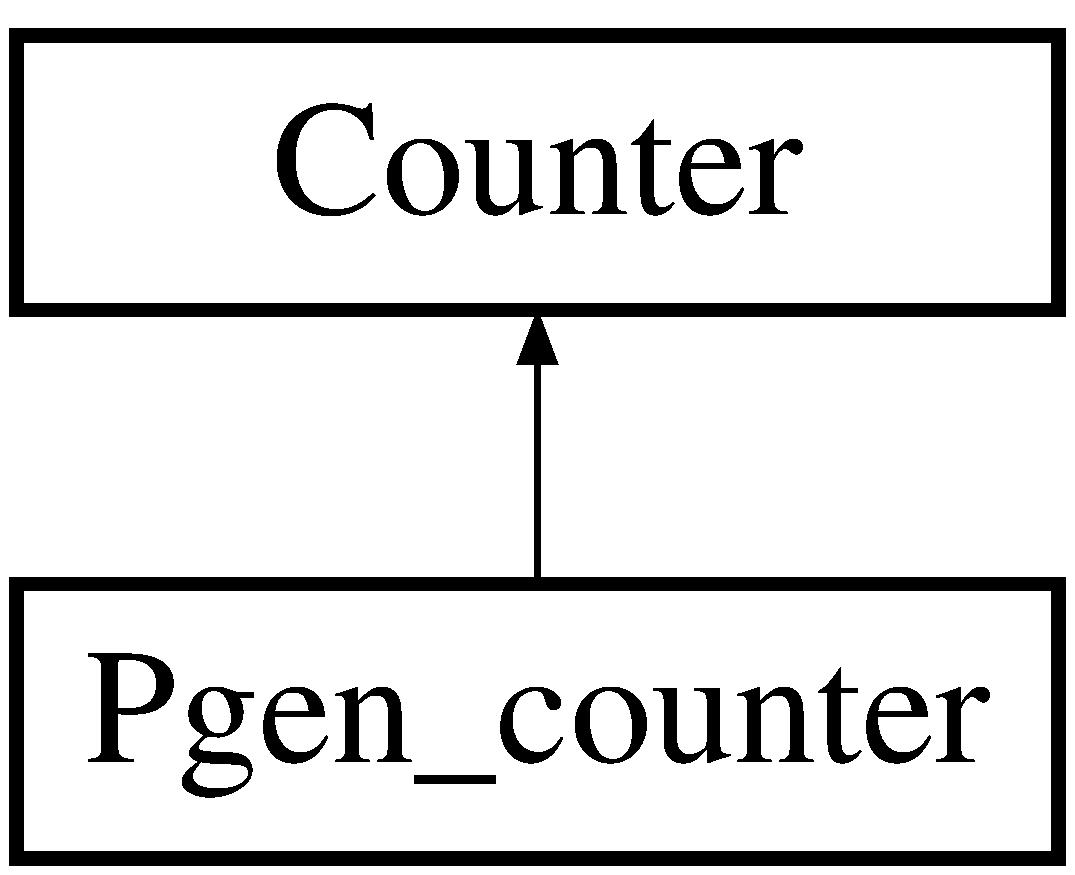
\includegraphics[height=2.000000cm]{d4/d57/classPgen__counter}
\end{center}
\end{figure}
\subsection*{Public Member Functions}
\begin{DoxyCompactItemize}
\item 
\mbox{\Hypertarget{classPgen__counter_a0c26a5a933018df8c7ceb94213004798}\label{classPgen__counter_a0c26a5a933018df8c7ceb94213004798}} 
{\bfseries Pgen\+\_\+counter} (std\+::string)
\item 
\mbox{\Hypertarget{classPgen__counter_a3291dde0930c68737fd791a2f1b2cc43}\label{classPgen__counter_a3291dde0930c68737fd791a2f1b2cc43}} 
{\bfseries Pgen\+\_\+counter} (std\+::string, bool, bool do\+\_\+output\+\_\+sequences=false)
\item 
\mbox{\Hypertarget{classPgen__counter_a6bc278117c83c8f797578c8b448f77cf}\label{classPgen__counter_a6bc278117c83c8f797578c8b448f77cf}} 
std\+::string {\bfseries type} () const
\item 
\mbox{\Hypertarget{classPgen__counter_a31b44277309564af777f79954438c8f1}\label{classPgen__counter_a31b44277309564af777f79954438c8f1}} 
void {\bfseries initialize\+\_\+counter} (const \hyperlink{classModel__Parms}{Model\+\_\+\+Parms} \&, const \hyperlink{classModel__marginals}{Model\+\_\+marginals} \&)
\item 
\mbox{\Hypertarget{classPgen__counter_a903fd5aed510d1f467ccda5fcf173a9a}\label{classPgen__counter_a903fd5aed510d1f467ccda5fcf173a9a}} 
void {\bfseries count\+\_\+scenario} (long double, double, const std\+::string \&, \hyperlink{classEnum__fast__memory__map}{Seq\+\_\+type\+\_\+str\+\_\+p\+\_\+map} \&, const \hyperlink{classEnum__fast__memory__dual__key__map}{Seq\+\_\+offsets\+\_\+map} \&, const std\+::unordered\+\_\+map$<$ std\+::tuple$<$ Event\+\_\+type, Gene\+\_\+class, Seq\+\_\+side $>$, std\+::shared\+\_\+ptr$<$ \hyperlink{classRec__Event}{Rec\+\_\+\+Event} $>$$>$ \&, \hyperlink{classEnum__fast__memory__map}{Mismatch\+\_\+vectors\+\_\+map} \&)
\item 
\mbox{\Hypertarget{classPgen__counter_a1884670498536b560eb019cb1514eba3}\label{classPgen__counter_a1884670498536b560eb019cb1514eba3}} 
void {\bfseries dump\+\_\+sequence\+\_\+data} (int, int)
\item 
\mbox{\Hypertarget{classPgen__counter_ade768bb6a0f87b139d7b5ae817ccb86d}\label{classPgen__counter_ade768bb6a0f87b139d7b5ae817ccb86d}} 
void {\bfseries add\+\_\+checked} (std\+::shared\+\_\+ptr$<$ \hyperlink{classCounter}{Counter} $>$)
\item 
\mbox{\Hypertarget{classPgen__counter_a2a2646dc8be803621c881038c8c34e11}\label{classPgen__counter_a2a2646dc8be803621c881038c8c34e11}} 
std\+::shared\+\_\+ptr$<$ \hyperlink{classCounter}{Counter} $>$ {\bfseries copy} () const
\end{DoxyCompactItemize}
\subsection*{Additional Inherited Members}


\subsection{Detailed Description}
Estimates sequences generation probability. 

\begin{DoxyAuthor}{Author}
Q.\+Marcou 
\end{DoxyAuthor}
\begin{DoxyVersion}{Version}
1.\+0
\end{DoxyVersion}
This \hyperlink{classCounter}{Counter} implements an estimator for the generation probability of evaluated sequences. Alternatively the counter can record the probability of generation of putative ancestor (unmutated/error free) sequences and their associated posterior probability. 

The documentation for this class was generated from the following files\+:\begin{DoxyCompactItemize}
\item 
Pgencounter.\+h\item 
Pgencounter.\+cpp\end{DoxyCompactItemize}

\hypertarget{classRec__Event}{}\section{Rec\+\_\+\+Event Class Reference}
\label{classRec__Event}\index{Rec\+\_\+\+Event@{Rec\+\_\+\+Event}}


Recombination event class (I\+GoR\textquotesingle{}s graph nodes)  




{\ttfamily \#include $<$Rec\+\_\+\+Event.\+h$>$}

Inheritance diagram for Rec\+\_\+\+Event\+:\begin{figure}[H]
\begin{center}
\leavevmode
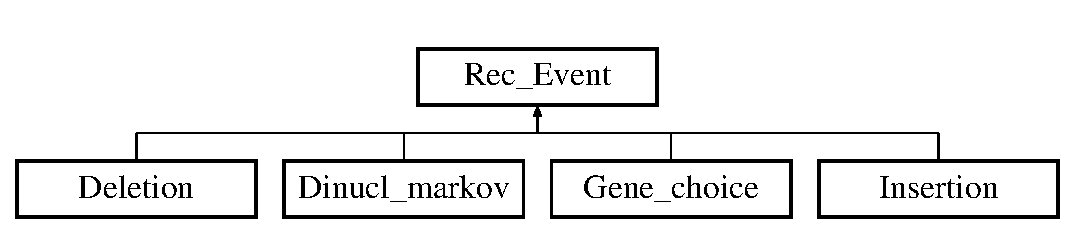
\includegraphics[height=2.000000cm]{dc/d20/classRec__Event}
\end{center}
\end{figure}
\subsection*{Public Member Functions}
\begin{DoxyCompactItemize}
\item 
\mbox{\Hypertarget{classRec__Event_a60eeeab16f772a796612ff3a74953b86}\label{classRec__Event_a60eeeab16f772a796612ff3a74953b86}} 
{\bfseries Rec\+\_\+\+Event} (Gene\+\_\+class, Seq\+\_\+side)
\item 
\mbox{\Hypertarget{classRec__Event_a13358de891bf06f564ed8848a364fffd}\label{classRec__Event_a13358de891bf06f564ed8848a364fffd}} 
{\bfseries Rec\+\_\+\+Event} (Gene\+\_\+class, Seq\+\_\+side, std\+::unordered\+\_\+map$<$ std\+::string, \hyperlink{structEvent__realization}{Event\+\_\+realization} $>$ \&)
\item 
\mbox{\Hypertarget{classRec__Event_ad4726690ef39967d2e2996f84d452f80}\label{classRec__Event_ad4726690ef39967d2e2996f84d452f80}} 
virtual std\+::shared\+\_\+ptr$<$ \hyperlink{classRec__Event}{Rec\+\_\+\+Event} $>$ {\bfseries copy} ()=0
\item 
\mbox{\Hypertarget{classRec__Event_a6786fc194b49fd7fd66a041f523b5fd8}\label{classRec__Event_a6786fc194b49fd7fd66a041f523b5fd8}} 
virtual int {\bfseries size} () const
\item 
virtual void \hyperlink{classRec__Event_a0fea607ec06bdd1a7f5ebb04a96e5253}{iterate} (double \&, \hyperlink{classEnum__fast__memory__map}{Downstream\+\_\+scenario\+\_\+proba\+\_\+bound\+\_\+map} \&, const std\+::string \&, const \hyperlink{classInt__Str}{Int\+\_\+\+Str} \&, \hyperlink{classEnum__fast__memory__map}{Index\+\_\+map} \&, const std\+::unordered\+\_\+map$<$ Rec\+\_\+\+Event\+\_\+name, std\+::vector$<$ std\+::pair$<$ std\+::shared\+\_\+ptr$<$ const \hyperlink{classRec__Event}{Rec\+\_\+\+Event} $>$, int $>$$>$$>$ \&, std\+::shared\+\_\+ptr$<$ \hyperlink{classRec__Event}{Next\+\_\+event\+\_\+ptr} $>$ \&, Marginal\+\_\+array\+\_\+p \&, const Marginal\+\_\+array\+\_\+p \&, const std\+::unordered\+\_\+map$<$ Gene\+\_\+class, std\+::vector$<$ \hyperlink{structAlignment__data}{Alignment\+\_\+data} $>$$>$ \&, \hyperlink{classEnum__fast__memory__map}{Seq\+\_\+type\+\_\+str\+\_\+p\+\_\+map} \&, \hyperlink{classEnum__fast__memory__dual__key__map}{Seq\+\_\+offsets\+\_\+map} \&, std\+::shared\+\_\+ptr$<$ \hyperlink{classError__rate}{Error\+\_\+rate} $>$ \&, std\+::map$<$ size\+\_\+t, std\+::shared\+\_\+ptr$<$ \hyperlink{classCounter}{Counter} $>$$>$ \&, const std\+::unordered\+\_\+map$<$ std\+::tuple$<$ Event\+\_\+type, Gene\+\_\+class, Seq\+\_\+side $>$, std\+::shared\+\_\+ptr$<$ \hyperlink{classRec__Event}{Rec\+\_\+\+Event} $>$$>$ \&, \hyperlink{classEnum__fast__memory__map}{Safety\+\_\+bool\+\_\+map} \&, \hyperlink{classEnum__fast__memory__map}{Mismatch\+\_\+vectors\+\_\+map} \&, double \&, double \&)=0
\begin{DoxyCompactList}\small\item\em Evaluate all Event\+\_\+\+Realization of a Rec\+Event for a given sequence. \end{DoxyCompactList}\item 
\mbox{\Hypertarget{classRec__Event_af256a2c82def78d75d41bc05e490da2f}\label{classRec__Event_af256a2c82def78d75d41bc05e490da2f}} 
bool {\bfseries set\+\_\+priority} (int)
\item 
\mbox{\Hypertarget{classRec__Event_ac835ea2ddf76b1a7741c4ed9bd156d2d}\label{classRec__Event_ac835ea2ddf76b1a7741c4ed9bd156d2d}} 
const Gene\+\_\+class {\bfseries get\+\_\+class} () const
\item 
\mbox{\Hypertarget{classRec__Event_a812462a0bb3d7b64589751ca005d9e38}\label{classRec__Event_a812462a0bb3d7b64589751ca005d9e38}} 
const Seq\+\_\+side {\bfseries get\+\_\+side} () const
\item 
\mbox{\Hypertarget{classRec__Event_ad4aa300c8b318c97934cbc87eb8d8145}\label{classRec__Event_ad4aa300c8b318c97934cbc87eb8d8145}} 
const std\+::unordered\+\_\+map$<$ std\+::string, \hyperlink{structEvent__realization}{Event\+\_\+realization} $>$ {\bfseries get\+\_\+realizations\+\_\+map} () const
\item 
\mbox{\Hypertarget{classRec__Event_ad4e1e82af3720042818e75344b68cd2d}\label{classRec__Event_ad4e1e82af3720042818e75344b68cd2d}} 
const int {\bfseries get\+\_\+priority} () const
\item 
\mbox{\Hypertarget{classRec__Event_a62d9a81d21710e36b890e3eb09e94969}\label{classRec__Event_a62d9a81d21710e36b890e3eb09e94969}} 
const Rec\+\_\+\+Event\+\_\+name {\bfseries get\+\_\+name} () const
\item 
\mbox{\Hypertarget{classRec__Event_a03d808075b0c4c3bf8cf2a1a0dfae326}\label{classRec__Event_a03d808075b0c4c3bf8cf2a1a0dfae326}} 
const std\+::string {\bfseries get\+\_\+nickname} () const
\item 
\mbox{\Hypertarget{classRec__Event_a0e512b4561e24468d257538eb02c71d3}\label{classRec__Event_a0e512b4561e24468d257538eb02c71d3}} 
void {\bfseries set\+\_\+nickname} (std\+::string name)
\item 
\mbox{\Hypertarget{classRec__Event_adda54fe71dcdacbacdd6115d4cc8af29}\label{classRec__Event_adda54fe71dcdacbacdd6115d4cc8af29}} 
Event\+\_\+type {\bfseries get\+\_\+type} () const
\item 
\mbox{\Hypertarget{classRec__Event_a0bb7fc872df04fc1c6710b608aa0b151}\label{classRec__Event_a0bb7fc872df04fc1c6710b608aa0b151}} 
int {\bfseries get\+\_\+len\+\_\+max} () const
\item 
\mbox{\Hypertarget{classRec__Event_af7df26b7168c20987a04db57fbe254f2}\label{classRec__Event_af7df26b7168c20987a04db57fbe254f2}} 
int {\bfseries get\+\_\+len\+\_\+min} () const
\item 
\mbox{\Hypertarget{classRec__Event_a28825288bde180aeba218c977ccabcfc}\label{classRec__Event_a28825288bde180aeba218c977ccabcfc}} 
bool {\bfseries operator==} (const \hyperlink{classRec__Event}{Rec\+\_\+\+Event} \&) const
\item 
\mbox{\Hypertarget{classRec__Event_a953dcbb13b233c32aa0613a849440445}\label{classRec__Event_a953dcbb13b233c32aa0613a849440445}} 
void {\bfseries update\+\_\+event\+\_\+name} ()
\item 
\mbox{\Hypertarget{classRec__Event_a8e6172c6c95a21fc90e8bbe4e2f6c46d}\label{classRec__Event_a8e6172c6c95a21fc90e8bbe4e2f6c46d}} 
virtual std\+::queue$<$ int $>$ {\bfseries draw\+\_\+random\+\_\+realization} (const Marginal\+\_\+array\+\_\+p \&, std\+::unordered\+\_\+map$<$ Rec\+\_\+\+Event\+\_\+name, int $>$ \&, const std\+::unordered\+\_\+map$<$ Rec\+\_\+\+Event\+\_\+name, std\+::vector$<$ std\+::pair$<$ std\+::shared\+\_\+ptr$<$ const \hyperlink{classRec__Event}{Rec\+\_\+\+Event} $>$, int $>$$>$$>$ \&, std\+::unordered\+\_\+map$<$ Seq\+\_\+type, std\+::string $>$ \&, std\+::mt19937\+\_\+64 \&) const =0
\item 
\mbox{\Hypertarget{classRec__Event_a48b16d4001f7b3fc6ad318fa91b24a37}\label{classRec__Event_a48b16d4001f7b3fc6ad318fa91b24a37}} 
virtual void {\bfseries write2txt} (std\+::ofstream \&)=0
\item 
\mbox{\Hypertarget{classRec__Event_ad44e71ab8c6451b52ed74efe8e141271}\label{classRec__Event_ad44e71ab8c6451b52ed74efe8e141271}} 
virtual void {\bfseries ind\+\_\+normalize} (Marginal\+\_\+array\+\_\+p \&, size\+\_\+t) const
\item 
\mbox{\Hypertarget{classRec__Event_a2b60dba9d85fce50fae2c0498c1725a0}\label{classRec__Event_a2b60dba9d85fce50fae2c0498c1725a0}} 
virtual void {\bfseries initialize\+\_\+event} (std\+::unordered\+\_\+set$<$ Rec\+\_\+\+Event\+\_\+name $>$ \&, const std\+::unordered\+\_\+map$<$ std\+::tuple$<$ Event\+\_\+type, Gene\+\_\+class, Seq\+\_\+side $>$, std\+::shared\+\_\+ptr$<$ \hyperlink{classRec__Event}{Rec\+\_\+\+Event} $>$$>$ \&, const std\+::unordered\+\_\+map$<$ Rec\+\_\+\+Event\+\_\+name, std\+::vector$<$ std\+::pair$<$ std\+::shared\+\_\+ptr$<$ const \hyperlink{classRec__Event}{Rec\+\_\+\+Event} $>$, int $>$$>$$>$ \&, \hyperlink{classEnum__fast__memory__map}{Downstream\+\_\+scenario\+\_\+proba\+\_\+bound\+\_\+map} \&, \hyperlink{classEnum__fast__memory__map}{Seq\+\_\+type\+\_\+str\+\_\+p\+\_\+map} \&, \hyperlink{classEnum__fast__memory__map}{Safety\+\_\+bool\+\_\+map} \&, std\+::shared\+\_\+ptr$<$ \hyperlink{classError__rate}{Error\+\_\+rate} $>$, \hyperlink{classEnum__fast__memory__map}{Mismatch\+\_\+vectors\+\_\+map} \&, \hyperlink{classEnum__fast__memory__dual__key__map}{Seq\+\_\+offsets\+\_\+map} \&, \hyperlink{classEnum__fast__memory__map}{Index\+\_\+map} \&)
\item 
\mbox{\Hypertarget{classRec__Event_ad1df9fff876350910e4085f67ba33ea2}\label{classRec__Event_ad1df9fff876350910e4085f67ba33ea2}} 
virtual void {\bfseries initialize\+\_\+crude\+\_\+scenario\+\_\+proba\+\_\+bound} (double \&, std\+::forward\+\_\+list$<$ double $\ast$$>$ \&, const std\+::unordered\+\_\+map$<$ std\+::tuple$<$ Event\+\_\+type, Gene\+\_\+class, Seq\+\_\+side $>$, std\+::shared\+\_\+ptr$<$ \hyperlink{classRec__Event}{Rec\+\_\+\+Event} $>$$>$ \&)
\item 
\mbox{\Hypertarget{classRec__Event_a16ba99854c015c6ae915814edba74b89}\label{classRec__Event_a16ba99854c015c6ae915814edba74b89}} 
virtual void {\bfseries add\+\_\+to\+\_\+marginals} (long double, Marginal\+\_\+array\+\_\+p \&) const =0
\item 
\mbox{\Hypertarget{classRec__Event_ac279e3c17ccd88ad7c64d2962da762fe}\label{classRec__Event_ac279e3c17ccd88ad7c64d2962da762fe}} 
virtual void {\bfseries set\+\_\+crude\+\_\+upper\+\_\+bound\+\_\+proba} (size\+\_\+t, size\+\_\+t, Marginal\+\_\+array\+\_\+p \&)
\item 
\mbox{\Hypertarget{classRec__Event_a0e31d0c1ee79f16b3e6232fa854730db}\label{classRec__Event_a0e31d0c1ee79f16b3e6232fa854730db}} 
void {\bfseries set\+\_\+upper\+\_\+bound\+\_\+proba} (double)
\item 
\mbox{\Hypertarget{classRec__Event_a52c29bfae989da81330569b45c6f5d81}\label{classRec__Event_a52c29bfae989da81330569b45c6f5d81}} 
double {\bfseries get\+\_\+upper\+\_\+bound\+\_\+proba} () const
\item 
virtual void \hyperlink{classRec__Event_a6b5b41f5d35969c61ba5fc90895203c3}{update\+\_\+event\+\_\+internal\+\_\+probas} (const Marginal\+\_\+array\+\_\+p \&, const std\+::unordered\+\_\+map$<$ Rec\+\_\+\+Event\+\_\+name, int $>$ \&)
\item 
\mbox{\Hypertarget{classRec__Event_a47dab56164c703538f2ce214e88a80f6}\label{classRec__Event_a47dab56164c703538f2ce214e88a80f6}} 
void {\bfseries set\+\_\+event\+\_\+identifier} (size\+\_\+t)
\item 
\mbox{\Hypertarget{classRec__Event_af6798049fbccee092bdd076b0db2c0a8}\label{classRec__Event_af6798049fbccee092bdd076b0db2c0a8}} 
int {\bfseries get\+\_\+event\+\_\+identifier} () const
\item 
\mbox{\Hypertarget{classRec__Event_aa5239e0c8d49b37c3e11e6d9554f47af}\label{classRec__Event_aa5239e0c8d49b37c3e11e6d9554f47af}} 
void {\bfseries set\+\_\+event\+\_\+marginal\+\_\+size} (size\+\_\+t ev\+\_\+size)
\item 
\mbox{\Hypertarget{classRec__Event_a191288063285122d7ce0bca6347bb469}\label{classRec__Event_a191288063285122d7ce0bca6347bb469}} 
bool {\bfseries is\+\_\+updated} () const
\item 
\mbox{\Hypertarget{classRec__Event_a1bd0021e7474ce38b0ff128a54e17634}\label{classRec__Event_a1bd0021e7474ce38b0ff128a54e17634}} 
void {\bfseries fix} (bool fix\+\_\+status)
\item 
\mbox{\Hypertarget{classRec__Event_a97f8b79a1d651b577ebebb8343dd0e4f}\label{classRec__Event_a97f8b79a1d651b577ebebb8343dd0e4f}} 
bool {\bfseries is\+\_\+fixed} () const
\item 
\mbox{\Hypertarget{classRec__Event_ad5c903886cabd9b5099ce3f9fca75721}\label{classRec__Event_ad5c903886cabd9b5099ce3f9fca75721}} 
void {\bfseries set\+\_\+viterbi\+\_\+run} (bool viterbi\+\_\+like)
\item 
\mbox{\Hypertarget{classRec__Event_aff100a79e69ebcf09302c9a6dd95e945}\label{classRec__Event_aff100a79e69ebcf09302c9a6dd95e945}} 
virtual double $\ast$ {\bfseries get\+\_\+updated\+\_\+ptr} ()
\item 
\mbox{\Hypertarget{classRec__Event_a0048d764ba437539343d7e5c7a3ab4bc}\label{classRec__Event_a0048d764ba437539343d7e5c7a3ab4bc}} 
void {\bfseries compute\+\_\+crude\+\_\+upper\+\_\+bound\+\_\+scenario\+\_\+proba} (double \&)
\item 
\mbox{\Hypertarget{classRec__Event_aa99c6c645054931943d9efe514684378}\label{classRec__Event_aa99c6c645054931943d9efe514684378}} 
const std\+::vector$<$ int $>$ \& {\bfseries get\+\_\+current\+\_\+realizations\+\_\+index\+\_\+vec} () const
\item 
\mbox{\Hypertarget{classRec__Event_ae241781e2135e31568bcd795af58588e}\label{classRec__Event_ae241781e2135e31568bcd795af58588e}} 
virtual bool {\bfseries has\+\_\+effect\+\_\+on} (Seq\+\_\+type) const =0
\item 
\mbox{\Hypertarget{classRec__Event_a12142d5ac5b5a0b19fe1bc32619247c9}\label{classRec__Event_a12142d5ac5b5a0b19fe1bc32619247c9}} 
void {\bfseries iterate\+\_\+initialize\+\_\+\+Len\+\_\+proba\+\_\+wrap\+\_\+up} (Seq\+\_\+type considered\+\_\+junction, std\+::map$<$ int, double $>$ \&length\+\_\+best\+\_\+proba\+\_\+map, std\+::queue$<$ std\+::shared\+\_\+ptr$<$ \hyperlink{classRec__Event}{Rec\+\_\+\+Event} $>$$>$ model\+\_\+queue, double scenario\+\_\+proba, const Marginal\+\_\+array\+\_\+p \&model\+\_\+parameters\+\_\+point, \hyperlink{classEnum__fast__memory__map}{Index\+\_\+map} \&base\+\_\+index\+\_\+map, \hyperlink{classEnum__fast__memory__map}{Seq\+\_\+type\+\_\+str\+\_\+p\+\_\+map} \&constructed\+\_\+sequences, int seq\+\_\+len) const
\item 
\mbox{\Hypertarget{classRec__Event_a49debedd11dbd2692cb8dbff233e4641}\label{classRec__Event_a49debedd11dbd2692cb8dbff233e4641}} 
virtual void {\bfseries iterate\+\_\+initialize\+\_\+\+Len\+\_\+proba} (Seq\+\_\+type considered\+\_\+junction, std\+::map$<$ int, double $>$ \&length\+\_\+best\+\_\+proba\+\_\+map, std\+::queue$<$ std\+::shared\+\_\+ptr$<$ \hyperlink{classRec__Event}{Rec\+\_\+\+Event} $>$$>$ \&model\+\_\+queue, double \&scenario\+\_\+proba, const Marginal\+\_\+array\+\_\+p \&model\+\_\+parameters\+\_\+point, \hyperlink{classEnum__fast__memory__map}{Index\+\_\+map} \&base\+\_\+index\+\_\+map, \hyperlink{classEnum__fast__memory__map}{Seq\+\_\+type\+\_\+str\+\_\+p\+\_\+map} \&constructed\+\_\+sequences, int \&seq\+\_\+len) const =0
\item 
\mbox{\Hypertarget{classRec__Event_a767dee38e8ddd93a328258d1394e00fc}\label{classRec__Event_a767dee38e8ddd93a328258d1394e00fc}} 
void {\bfseries iterate\+\_\+initialize\+\_\+\+Len\+\_\+proba} (Seq\+\_\+type considered\+\_\+junction, std\+::map$<$ int, double $>$ \&length\+\_\+best\+\_\+proba\+\_\+map, std\+::queue$<$ std\+::shared\+\_\+ptr$<$ \hyperlink{classRec__Event}{Rec\+\_\+\+Event} $>$$>$ \&model\+\_\+queue, double \&scenario\+\_\+proba, const Marginal\+\_\+array\+\_\+p \&model\+\_\+parameters\+\_\+point, \hyperlink{classEnum__fast__memory__map}{Index\+\_\+map} \&base\+\_\+index\+\_\+map, \hyperlink{classEnum__fast__memory__map}{Seq\+\_\+type\+\_\+str\+\_\+p\+\_\+map} \&constructed\+\_\+sequences) const
\item 
\mbox{\Hypertarget{classRec__Event_a82875bc17562b09142250db7f65844f2}\label{classRec__Event_a82875bc17562b09142250db7f65844f2}} 
virtual void {\bfseries initialize\+\_\+\+Len\+\_\+proba\+\_\+bound} (std\+::queue$<$ std\+::shared\+\_\+ptr$<$ \hyperlink{classRec__Event}{Rec\+\_\+\+Event} $>$$>$ \&model\+\_\+queue, const Marginal\+\_\+array\+\_\+p \&model\+\_\+parameters\+\_\+point, \hyperlink{classEnum__fast__memory__map}{Index\+\_\+map} \&base\+\_\+index\+\_\+map)=0
\end{DoxyCompactItemize}
\subsection*{Protected Member Functions}
\begin{DoxyCompactItemize}
\item 
\mbox{\Hypertarget{classRec__Event_ae55f294d71bd8f52cec13d318515b799}\label{classRec__Event_ae55f294d71bd8f52cec13d318515b799}} 
int {\bfseries compare\+\_\+sequences} (std\+::string, std\+::string)
\item 
\mbox{\Hypertarget{classRec__Event_a3aa2d2d685646b82cc04e25d3395e9ab}\label{classRec__Event_a3aa2d2d685646b82cc04e25d3395e9ab}} 
void {\bfseries add\+\_\+realization} (const \hyperlink{structEvent__realization}{Event\+\_\+realization} \&)
\item 
\mbox{\Hypertarget{classRec__Event_a0922f15959f097b4e1f1f4ef00c48d48}\label{classRec__Event_a0922f15959f097b4e1f1f4ef00c48d48}} 
void {\bfseries iterate\+\_\+wrap\+\_\+up} (double \&scenario\+\_\+proba, \hyperlink{classEnum__fast__memory__map}{Downstream\+\_\+scenario\+\_\+proba\+\_\+bound\+\_\+map} \&downstream\+\_\+proba\+\_\+map, const std\+::string \&sequence, const \hyperlink{classInt__Str}{Int\+\_\+\+Str} \&int\+\_\+sequence, \hyperlink{classEnum__fast__memory__map}{Index\+\_\+map} \&index\+\_\+map, const std\+::unordered\+\_\+map$<$ Rec\+\_\+\+Event\+\_\+name, std\+::vector$<$ std\+::pair$<$ std\+::shared\+\_\+ptr$<$ const \hyperlink{classRec__Event}{Rec\+\_\+\+Event} $>$, int $>$$>$$>$ \&offset\+\_\+map, std\+::shared\+\_\+ptr$<$ \hyperlink{classRec__Event}{Next\+\_\+event\+\_\+ptr} $>$ \&next\+\_\+event\+\_\+ptr\+\_\+arr, Marginal\+\_\+array\+\_\+p \&updated\+\_\+marginal\+\_\+array\+\_\+p, const Marginal\+\_\+array\+\_\+p \&model\+\_\+parameters\+\_\+point, const std\+::unordered\+\_\+map$<$ Gene\+\_\+class, std\+::vector$<$ \hyperlink{structAlignment__data}{Alignment\+\_\+data} $>$$>$ \&allowed\+\_\+realizations, \hyperlink{classEnum__fast__memory__map}{Seq\+\_\+type\+\_\+str\+\_\+p\+\_\+map} \&constructed\+\_\+sequences, \hyperlink{classEnum__fast__memory__dual__key__map}{Seq\+\_\+offsets\+\_\+map} \&seq\+\_\+offsets, std\+::shared\+\_\+ptr$<$ \hyperlink{classError__rate}{Error\+\_\+rate} $>$ \&error\+\_\+rate\+\_\+p, std\+::map$<$ size\+\_\+t, std\+::shared\+\_\+ptr$<$ \hyperlink{classCounter}{Counter} $>$$>$ \&counters\+\_\+list, const std\+::unordered\+\_\+map$<$ std\+::tuple$<$ Event\+\_\+type, Gene\+\_\+class, Seq\+\_\+side $>$, std\+::shared\+\_\+ptr$<$ \hyperlink{classRec__Event}{Rec\+\_\+\+Event} $>$$>$ \&events\+\_\+map, \hyperlink{classEnum__fast__memory__map}{Safety\+\_\+bool\+\_\+map} \&safety\+\_\+set, \hyperlink{classEnum__fast__memory__map}{Mismatch\+\_\+vectors\+\_\+map} \&mismatches\+\_\+lists, double \&seq\+\_\+max\+\_\+prob\+\_\+scenario, double \&proba\+\_\+threshold\+\_\+factor)
\end{DoxyCompactItemize}
\subsection*{Protected Attributes}
\begin{DoxyCompactItemize}
\item 
\mbox{\Hypertarget{classRec__Event_a07fc418d22098c2926653834fa0436c5}\label{classRec__Event_a07fc418d22098c2926653834fa0436c5}} 
std\+::unordered\+\_\+map$<$ std\+::string, \hyperlink{structEvent__realization}{Event\+\_\+realization} $>$ {\bfseries event\+\_\+realizations}
\item 
\mbox{\Hypertarget{classRec__Event_abd0cbac0857932ab119236558ca8fff2}\label{classRec__Event_abd0cbac0857932ab119236558ca8fff2}} 
int {\bfseries priority}
\item 
\mbox{\Hypertarget{classRec__Event_a484c20b2089a38fe1b265c8d01e6111e}\label{classRec__Event_a484c20b2089a38fe1b265c8d01e6111e}} 
Gene\+\_\+class {\bfseries event\+\_\+class}
\item 
\mbox{\Hypertarget{classRec__Event_a39522384697c7db8d3798d58e84740f1}\label{classRec__Event_a39522384697c7db8d3798d58e84740f1}} 
Seq\+\_\+side {\bfseries event\+\_\+side}
\item 
\mbox{\Hypertarget{classRec__Event_a4884eb9d3d3d08fb90e04e94dda014c4}\label{classRec__Event_a4884eb9d3d3d08fb90e04e94dda014c4}} 
Rec\+\_\+\+Event\+\_\+name {\bfseries name}
\item 
\mbox{\Hypertarget{classRec__Event_ad7a94cea0adcd33d96138b52520d3645}\label{classRec__Event_ad7a94cea0adcd33d96138b52520d3645}} 
std\+::string {\bfseries nickname}
\item 
\mbox{\Hypertarget{classRec__Event_ac90c7ca13ec2652ff60b6d8955608156}\label{classRec__Event_ac90c7ca13ec2652ff60b6d8955608156}} 
int {\bfseries len\+\_\+min}
\item 
\mbox{\Hypertarget{classRec__Event_a737c3083cf8b51493afbd81f4b77f32f}\label{classRec__Event_a737c3083cf8b51493afbd81f4b77f32f}} 
int {\bfseries len\+\_\+max}
\item 
\mbox{\Hypertarget{classRec__Event_a0c88bea7d614edcbc669e31f327bc526}\label{classRec__Event_a0c88bea7d614edcbc669e31f327bc526}} 
Event\+\_\+type {\bfseries type}
\item 
\mbox{\Hypertarget{classRec__Event_af2001da20d37833fde0796a925dd6a76}\label{classRec__Event_af2001da20d37833fde0796a925dd6a76}} 
int {\bfseries event\+\_\+index}
\item 
\mbox{\Hypertarget{classRec__Event_af6cfd37096cac09c44dc03284b8bbf37}\label{classRec__Event_af6cfd37096cac09c44dc03284b8bbf37}} 
std\+::forward\+\_\+list$<$ std\+::tuple$<$ int, int, int $>$ $>$ {\bfseries memory\+\_\+and\+\_\+offsets}
\item 
\mbox{\Hypertarget{classRec__Event_a4fbeb3694cf3a3ef3097ec2af5e96f3c}\label{classRec__Event_a4fbeb3694cf3a3ef3097ec2af5e96f3c}} 
bool {\bfseries updated}
\item 
\mbox{\Hypertarget{classRec__Event_a877417ca96bc33491b73ef9f60c8f9eb}\label{classRec__Event_a877417ca96bc33491b73ef9f60c8f9eb}} 
bool {\bfseries viterbi\+\_\+run}
\item 
\mbox{\Hypertarget{classRec__Event_a835244ce395c153efca8e5b9dff73f06}\label{classRec__Event_a835244ce395c153efca8e5b9dff73f06}} 
bool {\bfseries initialized}
\item 
\mbox{\Hypertarget{classRec__Event_ae18d91f49ea6652853f9c620a3cf2005}\label{classRec__Event_ae18d91f49ea6652853f9c620a3cf2005}} 
size\+\_\+t {\bfseries event\+\_\+marginal\+\_\+size}
\item 
\mbox{\Hypertarget{classRec__Event_a337f07555611e2d37b962e5e8d4915a6}\label{classRec__Event_a337f07555611e2d37b962e5e8d4915a6}} 
bool {\bfseries fixed}
\item 
\mbox{\Hypertarget{classRec__Event_a6ce94f7d653f284678bb31462257579e}\label{classRec__Event_a6ce94f7d653f284678bb31462257579e}} 
double {\bfseries event\+\_\+upper\+\_\+bound\+\_\+proba}
\item 
\mbox{\Hypertarget{classRec__Event_a6631657503c1b5cd5e6b55cef3bb2c55}\label{classRec__Event_a6631657503c1b5cd5e6b55cef3bb2c55}} 
double {\bfseries scenario\+\_\+downstream\+\_\+upper\+\_\+bound\+\_\+proba}
\item 
\mbox{\Hypertarget{classRec__Event_a3ed5d1bcf4a2ca83aebb2e81c0d9a06b}\label{classRec__Event_a3ed5d1bcf4a2ca83aebb2e81c0d9a06b}} 
double {\bfseries scenario\+\_\+upper\+\_\+bound\+\_\+proba}
\item 
\mbox{\Hypertarget{classRec__Event_a23ef7bc59131d34ace470c9bea042e66}\label{classRec__Event_a23ef7bc59131d34ace470c9bea042e66}} 
std\+::forward\+\_\+list$<$ double $\ast$ $>$ {\bfseries updated\+\_\+proba\+\_\+bounds\+\_\+list}
\item 
\mbox{\Hypertarget{classRec__Event_a38998c66aa7e4b29284f4c8f35cabbc6}\label{classRec__Event_a38998c66aa7e4b29284f4c8f35cabbc6}} 
std\+::vector$<$ int $>$ {\bfseries current\+\_\+realizations\+\_\+index\+\_\+vec}
\item 
\mbox{\Hypertarget{classRec__Event_a57f8109e6fdbee1590cd1a6ddf62242a}\label{classRec__Event_a57f8109e6fdbee1590cd1a6ddf62242a}} 
const int $\ast$ {\bfseries current\+\_\+realization\+\_\+index}
\item 
\mbox{\Hypertarget{classRec__Event_afaac2c8eb6698209ab356b892e379000}\label{classRec__Event_afaac2c8eb6698209ab356b892e379000}} 
int {\bfseries current\+\_\+downstream\+\_\+proba\+\_\+memory\+\_\+layers} \mbox{[}6\mbox{]}
\end{DoxyCompactItemize}


\subsection{Detailed Description}
Recombination event class (I\+GoR\textquotesingle{}s graph nodes) 

\begin{DoxyAuthor}{Author}
Q.\+Marcou 
\end{DoxyAuthor}
\begin{DoxyVersion}{Version}
1.\+0
\end{DoxyVersion}
This class implements the recombination event object. Rec\+\_\+\+Events are the nodes in I\+GoR\textquotesingle{}s Bayesian Network structure. This is a purely abstract class and cannot be instanciated as is, only classes deriving from it and implementing the purely abstract methods can be.

Rec\+\_\+\+Events contain the different \hyperlink{structEvent__realization}{Event\+\_\+realization} associated to it in a hashmap.

The Rec\+Events design is key to the way I\+GoR explore all possible scenarios (through the iterate method) and generate sequences (through the draw\+\_\+random\+\_\+realization) 

\subsection{Member Function Documentation}
\mbox{\Hypertarget{classRec__Event_a0fea607ec06bdd1a7f5ebb04a96e5253}\label{classRec__Event_a0fea607ec06bdd1a7f5ebb04a96e5253}} 
\index{Rec\+\_\+\+Event@{Rec\+\_\+\+Event}!iterate@{iterate}}
\index{iterate@{iterate}!Rec\+\_\+\+Event@{Rec\+\_\+\+Event}}
\subsubsection{\texorpdfstring{iterate()}{iterate()}}
{\footnotesize\ttfamily virtual void Rec\+\_\+\+Event\+::iterate (\begin{DoxyParamCaption}\item[{double \&}]{,  }\item[{\hyperlink{classEnum__fast__memory__map}{Downstream\+\_\+scenario\+\_\+proba\+\_\+bound\+\_\+map} \&}]{,  }\item[{const std\+::string \&}]{,  }\item[{const \hyperlink{classInt__Str}{Int\+\_\+\+Str} \&}]{,  }\item[{\hyperlink{classEnum__fast__memory__map}{Index\+\_\+map} \&}]{,  }\item[{const std\+::unordered\+\_\+map$<$ Rec\+\_\+\+Event\+\_\+name, std\+::vector$<$ std\+::pair$<$ std\+::shared\+\_\+ptr$<$ const \hyperlink{classRec__Event}{Rec\+\_\+\+Event} $>$, int $>$$>$$>$ \&}]{,  }\item[{std\+::shared\+\_\+ptr$<$ \hyperlink{classRec__Event}{Next\+\_\+event\+\_\+ptr} $>$ \&}]{,  }\item[{Marginal\+\_\+array\+\_\+p \&}]{,  }\item[{const Marginal\+\_\+array\+\_\+p \&}]{,  }\item[{const std\+::unordered\+\_\+map$<$ Gene\+\_\+class, std\+::vector$<$ \hyperlink{structAlignment__data}{Alignment\+\_\+data} $>$$>$ \&}]{,  }\item[{\hyperlink{classEnum__fast__memory__map}{Seq\+\_\+type\+\_\+str\+\_\+p\+\_\+map} \&}]{,  }\item[{\hyperlink{classEnum__fast__memory__dual__key__map}{Seq\+\_\+offsets\+\_\+map} \&}]{,  }\item[{std\+::shared\+\_\+ptr$<$ \hyperlink{classError__rate}{Error\+\_\+rate} $>$ \&}]{,  }\item[{std\+::map$<$ size\+\_\+t, std\+::shared\+\_\+ptr$<$ \hyperlink{classCounter}{Counter} $>$$>$ \&}]{,  }\item[{const std\+::unordered\+\_\+map$<$ std\+::tuple$<$ Event\+\_\+type, Gene\+\_\+class, Seq\+\_\+side $>$, std\+::shared\+\_\+ptr$<$ \hyperlink{classRec__Event}{Rec\+\_\+\+Event} $>$$>$ \&}]{,  }\item[{\hyperlink{classEnum__fast__memory__map}{Safety\+\_\+bool\+\_\+map} \&}]{,  }\item[{\hyperlink{classEnum__fast__memory__map}{Mismatch\+\_\+vectors\+\_\+map} \&}]{,  }\item[{double \&}]{,  }\item[{double \&}]{ }\end{DoxyParamCaption})\hspace{0.3cm}{\ttfamily [pure virtual]}}



Evaluate all Event\+\_\+\+Realization of a Rec\+Event for a given sequence. 

\begin{DoxyAuthor}{Author}
Q.\+Marcou 
\end{DoxyAuthor}
\begin{DoxyVersion}{Version}
1.\+0 
\end{DoxyVersion}

\begin{DoxyParams}[1]{Parameters}
\mbox{\tt in,out}  & {\em scenario\+\_\+proba} & Probability of the currently explored (incomplete) scenario \\
\hline
\mbox{\tt in,out}  & {\em downstream\+\_\+proba\+\_\+map} & \\
\hline
\mbox{\tt in}  & {\em sequence} & The studied sequence in nucleotide code \\
\hline
\mbox{\tt in}  & {\em int\+\_\+sequence} & The studied sequence in integer code \\
\hline
\mbox{\tt in,out}  & {\em base\+\_\+index\+\_\+map} & Dynamic map recording where probabilities should be read on the marginals. \\
\hline
\mbox{\tt in}  & {\em offset\+\_\+map} & Tells the event by how much indices from the children events should be modified \\
\hline
\mbox{\tt in}  & {\em next\+\_\+event\+\_\+ptr\+\_\+arr} & Indicates the next event to call iterate on \\
\hline
\mbox{\tt in}  & {\em updated\+\_\+marginals\+\_\+point} & Summary marginals on which complete scenario posteriors are recorded \\
\hline
\mbox{\tt in}  & {\em model\+\_\+parameters\+\_\+point} & Current recombination probability distribution \\
\hline
\mbox{\tt in}  & {\em allowed\+\_\+realizations} & The set of genomic templates alignment \\
\hline
\mbox{\tt in,out}  & {\em constructed\+\_\+sequences} & Map containing the (incomplete) scenario\textquotesingle{}s resulting sequence \\
\hline
\mbox{\tt in,out}  & {\em seq\+\_\+offsets} & Map containing the 3\textquotesingle{} and 5\textquotesingle{} offsets of each scenario sequence piece \\
\hline
\mbox{\tt in}  & {\em error\+\_\+rate\+\_\+p} & Pointer to the error model object \\
\hline
\mbox{\tt in}  & {\em counters\+\_\+list} & The list of \hyperlink{classCounter}{Counter} to be counted \\
\hline
\mbox{\tt in}  & {\em events\+\_\+map} & A map containing all events contained in the Model\+\_\+parms, accessible through their type, gene class and side. \\
\hline
\mbox{\tt in,out}  & {\em safety\+\_\+set} & A map indicating whether checks on offsets overlap should be performed \\
\hline
\mbox{\tt in,out}  & {\em mismatches\+\_\+lists} & A map containing the (incomplete) scenario mismatches \\
\hline
\mbox{\tt in}  & {\em seq\+\_\+max\+\_\+prob\+\_\+scenario} & Most likely scenario\textquotesingle{}s probability for the considered sequence \\
\hline
\mbox{\tt in}  & {\em proba\+\_\+threshold\+\_\+factor} & Threshold on probability ratio between most likely scenario and explored scenario\\
\hline
\end{DoxyParams}
\begin{DoxyReturn}{Returns}
void
\end{DoxyReturn}
The iterate method is the heart of I\+GoR\textquotesingle{}s scenario exploration. \hyperlink{classModel__Parms}{Model\+\_\+\+Parms} define an order in which the Rec\+Event should be processed. Upon call of iterate all Event\+Realization of the Rec\+Event are assessed and for each possible realization the iterate method is called recursively for the next event. Inside the iterate method a filtering on too improbable realizations is performed (tree prunning) using the downstream\+\_\+proba\+\_\+map.

The index map is used to read off the probability of the current Rec\+Event Event\+Realization at the correct location given the events parent\textquotesingle{}s realizations. It is further modified to take into account the current event\textquotesingle{}s realization when its children realization probabilities will be read. 

Implemented in \hyperlink{classDeletion_a2479968a06062e87027f8acef2631211}{Deletion}, \hyperlink{classDinucl__markov_ace49d0da113be7d77ad0d4c3b8152c3d}{Dinucl\+\_\+markov}, \hyperlink{classGene__choice_ab036f686e32561d4db2aa9eca3be4cf0}{Gene\+\_\+choice}, and \hyperlink{classInsertion_a9c0f15989a298d7ddf7311c432f995b9}{Insertion}.

\mbox{\Hypertarget{classRec__Event_a6b5b41f5d35969c61ba5fc90895203c3}\label{classRec__Event_a6b5b41f5d35969c61ba5fc90895203c3}} 
\index{Rec\+\_\+\+Event@{Rec\+\_\+\+Event}!update\+\_\+event\+\_\+internal\+\_\+probas@{update\+\_\+event\+\_\+internal\+\_\+probas}}
\index{update\+\_\+event\+\_\+internal\+\_\+probas@{update\+\_\+event\+\_\+internal\+\_\+probas}!Rec\+\_\+\+Event@{Rec\+\_\+\+Event}}
\subsubsection{\texorpdfstring{update\+\_\+event\+\_\+internal\+\_\+probas()}{update\_event\_internal\_probas()}}
{\footnotesize\ttfamily void Rec\+\_\+\+Event\+::update\+\_\+event\+\_\+internal\+\_\+probas (\begin{DoxyParamCaption}\item[{const Marginal\+\_\+array\+\_\+p \&}]{,  }\item[{const std\+::unordered\+\_\+map$<$ Rec\+\_\+\+Event\+\_\+name, int $>$ \&}]{ }\end{DoxyParamCaption})\hspace{0.3cm}{\ttfamily [virtual]}}

Does nothing since in general events will not need to perform any operation on the marginal probabilities 

Reimplemented in \hyperlink{classDinucl__markov_a8da33acb0a389a0a4c845a69c11b173c}{Dinucl\+\_\+markov}.



The documentation for this class was generated from the following files\+:\begin{DoxyCompactItemize}
\item 
Rec\+\_\+\+Event.\+h\item 
Rec\+\_\+\+Event.\+cpp\end{DoxyCompactItemize}

\hypertarget{classSingle__error__rate}{}\section{Single\+\_\+error\+\_\+rate Class Reference}
\label{classSingle__error__rate}\index{Single\+\_\+error\+\_\+rate@{Single\+\_\+error\+\_\+rate}}


Independent single nucleotide error model.  




{\ttfamily \#include $<$Singleerrorrate.\+h$>$}

Inheritance diagram for Single\+\_\+error\+\_\+rate\+:\begin{figure}[H]
\begin{center}
\leavevmode
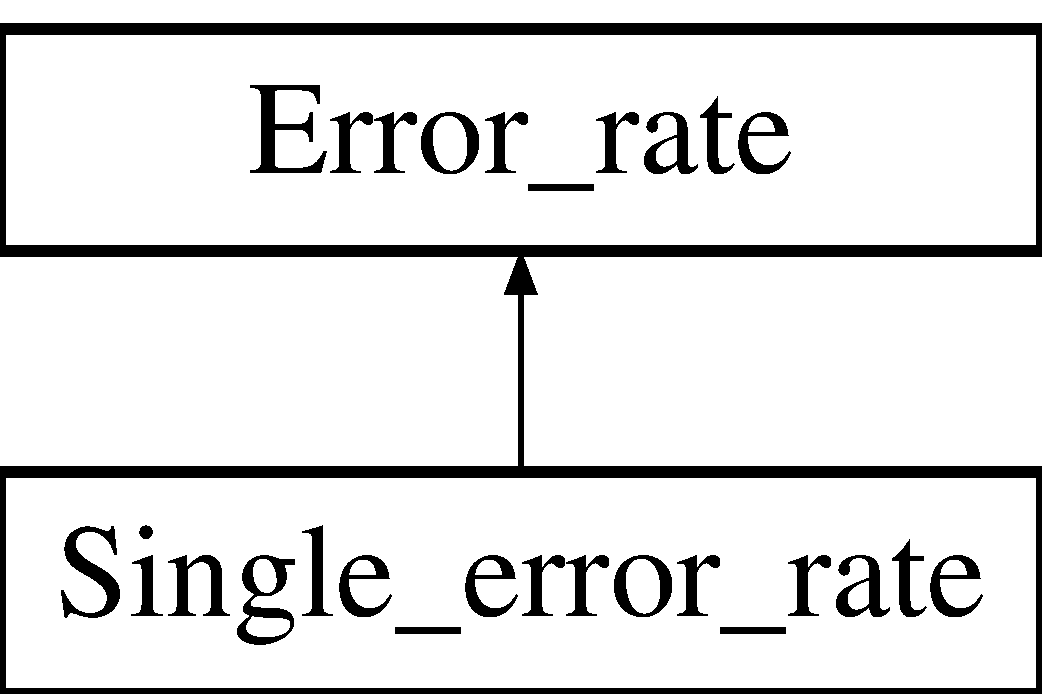
\includegraphics[height=2.000000cm]{d5/de1/classSingle__error__rate}
\end{center}
\end{figure}
\subsection*{Public Member Functions}
\begin{DoxyCompactItemize}
\item 
\mbox{\Hypertarget{classSingle__error__rate_a687686cd400935103647436b27984330}\label{classSingle__error__rate_a687686cd400935103647436b27984330}} 
{\bfseries Single\+\_\+error\+\_\+rate} (double)
\item 
\mbox{\Hypertarget{classSingle__error__rate_a142d9c5ad52f1f6fa20565c42158a426}\label{classSingle__error__rate_a142d9c5ad52f1f6fa20565c42158a426}} 
double {\bfseries compare\+\_\+sequences\+\_\+error\+\_\+prob} (double, const std\+::string \&, \hyperlink{classEnum__fast__memory__map}{Seq\+\_\+type\+\_\+str\+\_\+p\+\_\+map} \&, const \hyperlink{classEnum__fast__memory__dual__key__map}{Seq\+\_\+offsets\+\_\+map} \&, const std\+::unordered\+\_\+map$<$ std\+::tuple$<$ Event\+\_\+type, Gene\+\_\+class, Seq\+\_\+side $>$, std\+::shared\+\_\+ptr$<$ \hyperlink{classRec__Event}{Rec\+\_\+\+Event} $>$$>$ \&, \hyperlink{classEnum__fast__memory__map}{Mismatch\+\_\+vectors\+\_\+map} \&, double \&, double \&)
\item 
\mbox{\Hypertarget{classSingle__error__rate_a0d4fb62ed45df43f95d7f85e5150639f}\label{classSingle__error__rate_a0d4fb62ed45df43f95d7f85e5150639f}} 
void {\bfseries update} ()
\item 
\mbox{\Hypertarget{classSingle__error__rate_afb8ba0c35a20ff9c83d71eadc21013c7}\label{classSingle__error__rate_afb8ba0c35a20ff9c83d71eadc21013c7}} 
void {\bfseries add\+\_\+to\+\_\+norm\+\_\+counter} ()
\item 
\mbox{\Hypertarget{classSingle__error__rate_a0d6d6f3ce09bf9a9a01426557bc11075}\label{classSingle__error__rate_a0d6d6f3ce09bf9a9a01426557bc11075}} 
void {\bfseries clean\+\_\+seq\+\_\+counters} ()
\item 
\mbox{\Hypertarget{classSingle__error__rate_ac5d91ac7d2fbd646210a04a7f56df00d}\label{classSingle__error__rate_ac5d91ac7d2fbd646210a04a7f56df00d}} 
\hyperlink{classSingle__error__rate}{Single\+\_\+error\+\_\+rate} {\bfseries operator+} (\hyperlink{classSingle__error__rate}{Single\+\_\+error\+\_\+rate})
\item 
\mbox{\Hypertarget{classSingle__error__rate_a34faf13d5f4a2fca1c2acc8bc69b23c7}\label{classSingle__error__rate_a34faf13d5f4a2fca1c2acc8bc69b23c7}} 
\hyperlink{classSingle__error__rate}{Single\+\_\+error\+\_\+rate} \& {\bfseries operator+=} (\hyperlink{classSingle__error__rate}{Single\+\_\+error\+\_\+rate})
\item 
\mbox{\Hypertarget{classSingle__error__rate_a5779a63cac826ae4c170cf61f1d7a13f}\label{classSingle__error__rate_a5779a63cac826ae4c170cf61f1d7a13f}} 
void {\bfseries write2txt} (std\+::ofstream \&)
\item 
\mbox{\Hypertarget{classSingle__error__rate_aa61f2543536c155ec67e1f03e3bda900}\label{classSingle__error__rate_aa61f2543536c155ec67e1f03e3bda900}} 
std\+::shared\+\_\+ptr$<$ \hyperlink{classError__rate}{Error\+\_\+rate} $>$ {\bfseries copy} () const
\item 
\mbox{\Hypertarget{classSingle__error__rate_af1d43b6aab1fdc5302d3a26479f83e7f}\label{classSingle__error__rate_af1d43b6aab1fdc5302d3a26479f83e7f}} 
std\+::string {\bfseries type} () const
\item 
\mbox{\Hypertarget{classSingle__error__rate_ada7e9b73b47acff05366d2fefeb4a1f2}\label{classSingle__error__rate_ada7e9b73b47acff05366d2fefeb4a1f2}} 
\hyperlink{classError__rate}{Error\+\_\+rate} $\ast$ {\bfseries add\+\_\+checked} (\hyperlink{classError__rate}{Error\+\_\+rate} $\ast$)
\item 
\mbox{\Hypertarget{classSingle__error__rate_ac378550cb29fb1449ce17a6184a553e9}\label{classSingle__error__rate_ac378550cb29fb1449ce17a6184a553e9}} 
const double \& {\bfseries get\+\_\+err\+\_\+rate\+\_\+upper\+\_\+bound} (size\+\_\+t, size\+\_\+t)
\item 
\mbox{\Hypertarget{classSingle__error__rate_a3bff9288c541e920e76ba34c50e6b16a}\label{classSingle__error__rate_a3bff9288c541e920e76ba34c50e6b16a}} 
void {\bfseries build\+\_\+upper\+\_\+bound\+\_\+matrix} (size\+\_\+t, size\+\_\+t)
\item 
\mbox{\Hypertarget{classSingle__error__rate_a629d245c987f0b9b7cd6f80aeea6d69c}\label{classSingle__error__rate_a629d245c987f0b9b7cd6f80aeea6d69c}} 
int {\bfseries get\+\_\+number\+\_\+non\+\_\+zero\+\_\+likelihood\+\_\+seqs} () const
\item 
\mbox{\Hypertarget{classSingle__error__rate_a536ce634d01c251251961bd463a57da4}\label{classSingle__error__rate_a536ce634d01c251251961bd463a57da4}} 
std\+::queue$<$ int $>$ {\bfseries generate\+\_\+errors} (std\+::string \&, std\+::mt19937\+\_\+64 \&) const
\end{DoxyCompactItemize}
\subsection*{Additional Inherited Members}


\subsection{Detailed Description}
Independent single nucleotide error model. 

\begin{DoxyAuthor}{Author}
Q.\+Marcou 
\end{DoxyAuthor}
\begin{DoxyVersion}{Version}
1.\+0
\end{DoxyVersion}
Simplest instance of the Error\+Rate family. Models errors/mutations as a Bernouilli process with a global rate independent of position and context. 

The documentation for this class was generated from the following files\+:\begin{DoxyCompactItemize}
\item 
Singleerrorrate.\+h\item 
Singleerrorrate.\+cpp\end{DoxyCompactItemize}

%--- End generated contents ---

% Index
\backmatter
\newpage
\phantomsection
\clearemptydoublepage
\addcontentsline{toc}{chapter}{Index}
\printindex

\end{document}
